This section presents verification and performance results of the standard and hybrid FEM-BEM coupling schemes, for molecules modeled as cavities with constant and varying permittivity.
When the permittivity inside the molecule was constant, we tested convergence against the available analytical expression of the solvation energy of a sphere [Kirkwood1934], and then compared a more realistic geometry (arginine) with a purely BEM implementation.
On the other hand, we considered a Gaussian-varying permittivity [Alexov and earlier] inside arginine, and used APBS [Baker2001] to verify.
The final result of this section shows the scaling of the standard and hybrid FEM-BEM coupling, as the molecule size grows. 

All runs were done on XX computer with YY specifications. 

\section*{\sffamily \Large Results with constant permitivitty}

In implicit-solvent models, the molecule is usually considered as a region with constant permittivity, in this case, with $\epsilon_1=4$.
In the solvent region, we used the permittivity of water ($\epsilon_2$=80) and an inverse of the Debye length of $\kappa=0.125$ \AA$^{-1}$.

\subsection*{\sffamily \large Convergence of a spherical cavity}

The Kirkwood sphere [Kirkwood1934] is a standard benchmarck for the Poisson-Boltzmann equation in molecular electrostatics. 
Here, we considered a spherical cavity with radius $R=2$ \AA, with three charges ($q_1$=1, $q_2$=1, and $q_3$=0.75) placed at $\mathbf{x}_1=(1,0,0)$, $\mathbf{x}_2=(0.7,0.7,0)$, and $\mathbf{x}_3=(-0.5,-0.5,0)$.
Figure \ref{fig:error_sphere} shows the error convergence of the standard and hybrid FEM-BEM approaches, and a reference BEM implementation, to the analytical solution ($\Delta G_{solv}= -164.33752347454015$ kcal/mol). 
In these runs, the FEM mesh was generated using Bempp (check?) from a surface discretization with W, X, Y, and Z vertices per \AA$^2$ on the SES, which was also used for the BEM runs. 
For the hybrid FEM-BEM coupling approach, we used $\tau$=10.

The error in Figure \ref{fig:error_sphere} decays linearly with the surface area, which agrees with the expected convergence for P1 elements, indicating a correct implementation of the numerical scheme. 
We can see that the purely BEM implementation outperforms (or not?) FEM-BEM coupling in terms of accuracy for equivalent meshes, and also that the hybrid approach does not (or does?) influence accuracy. 

\begin{figure}
  \centering
  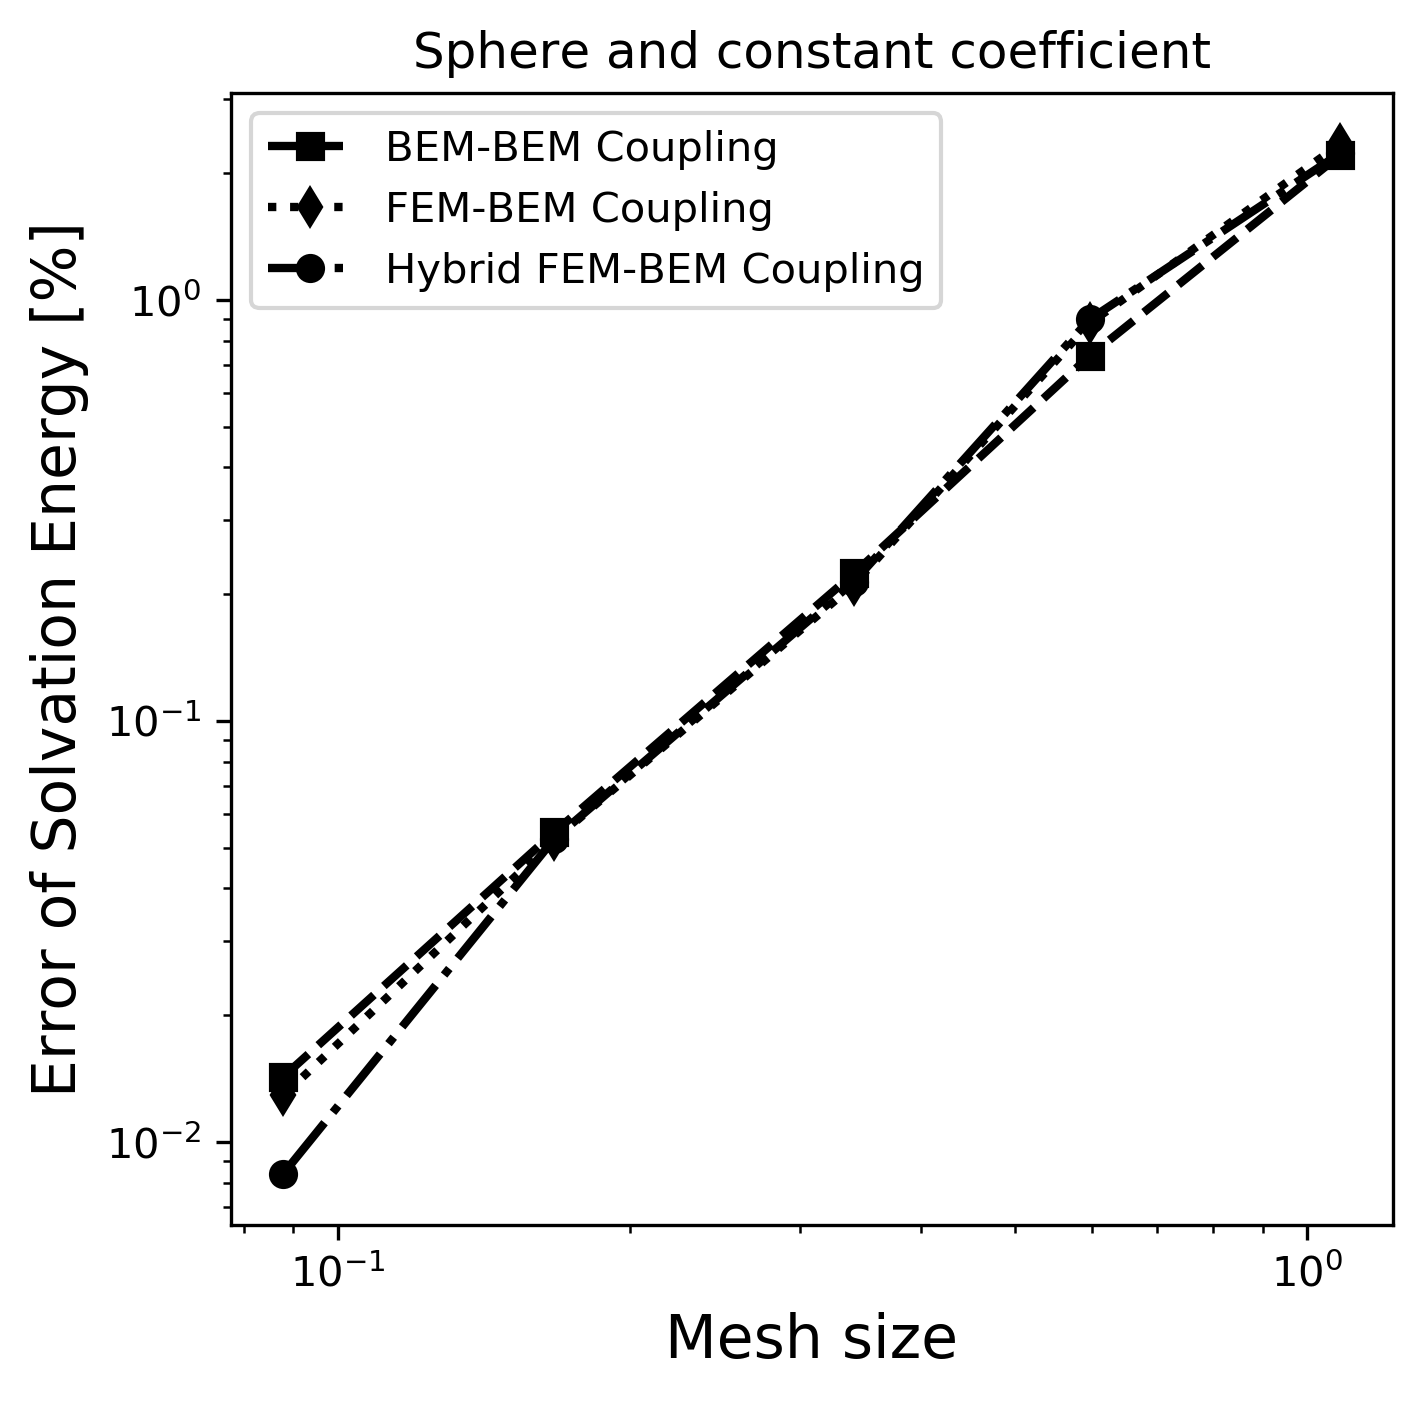
\includegraphics[width=0.6\linewidth]{Sphere_const_coeff_error.png}
%   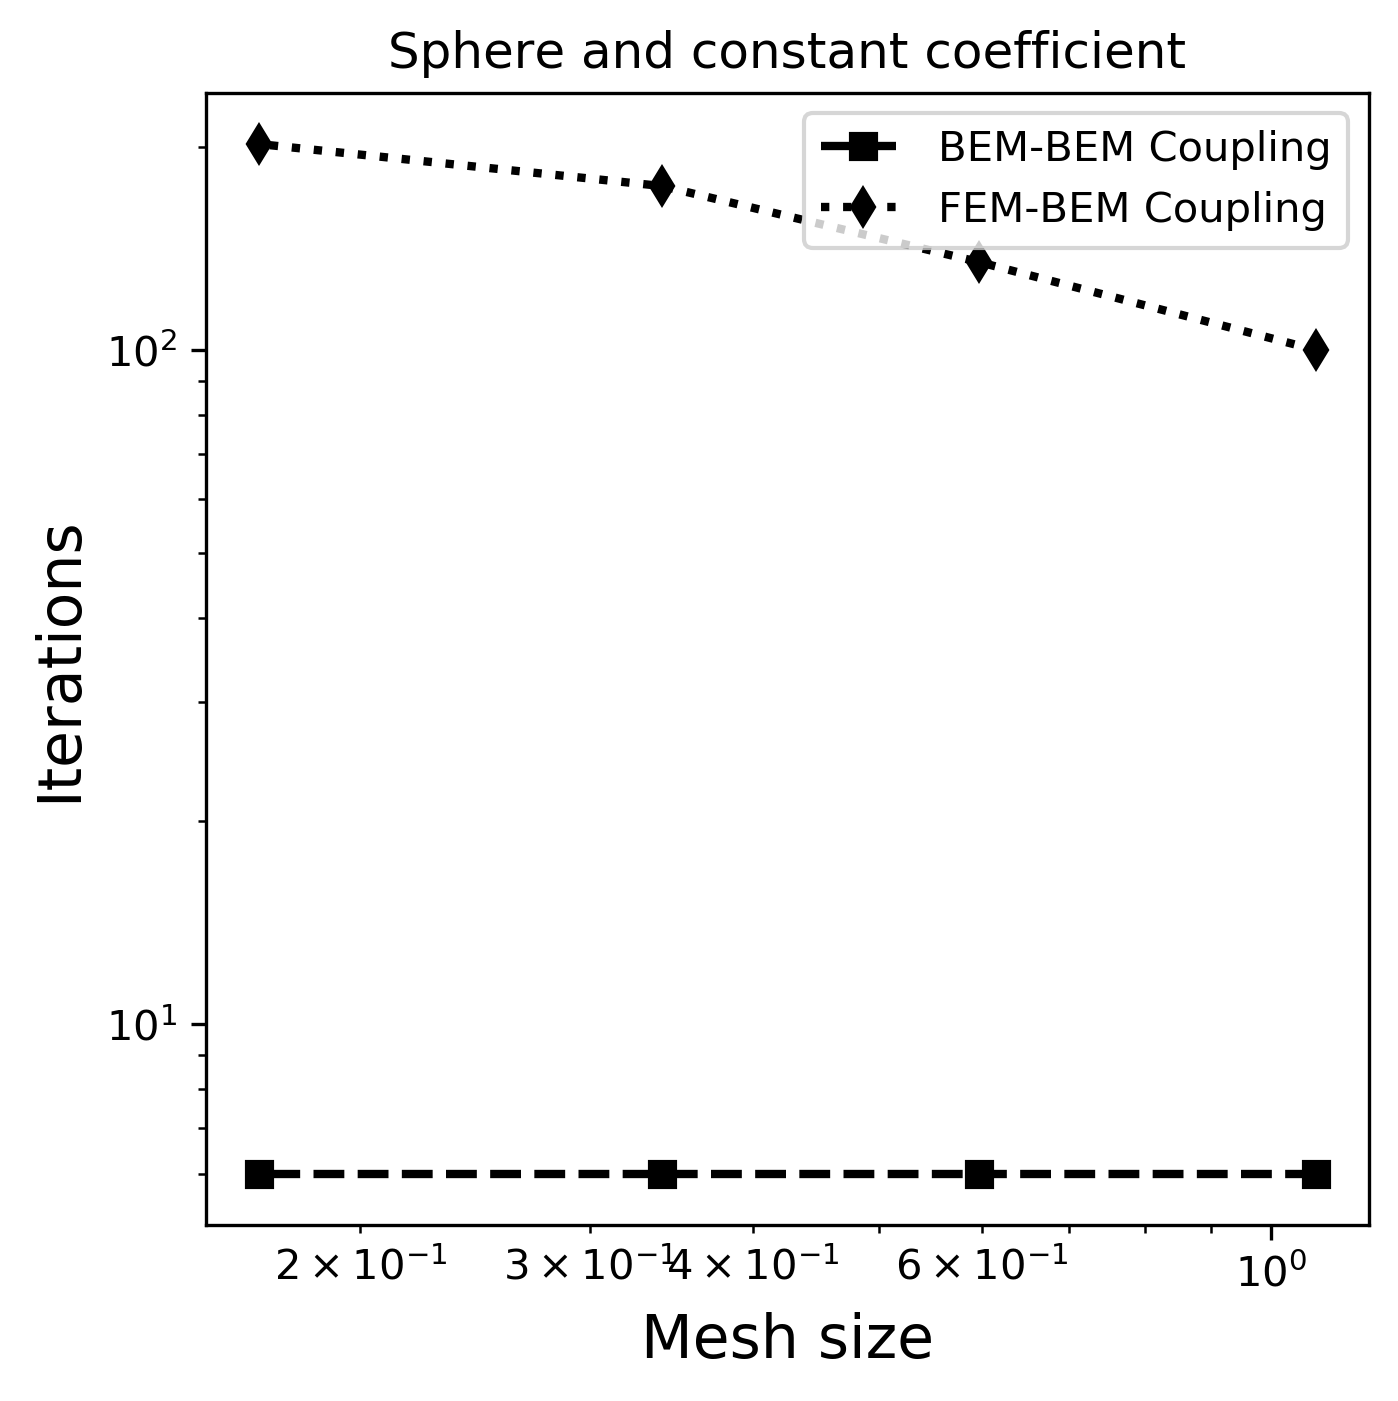
\includegraphics[width=0.45\linewidth]{Sphere_const_coeff_iter.png}
%   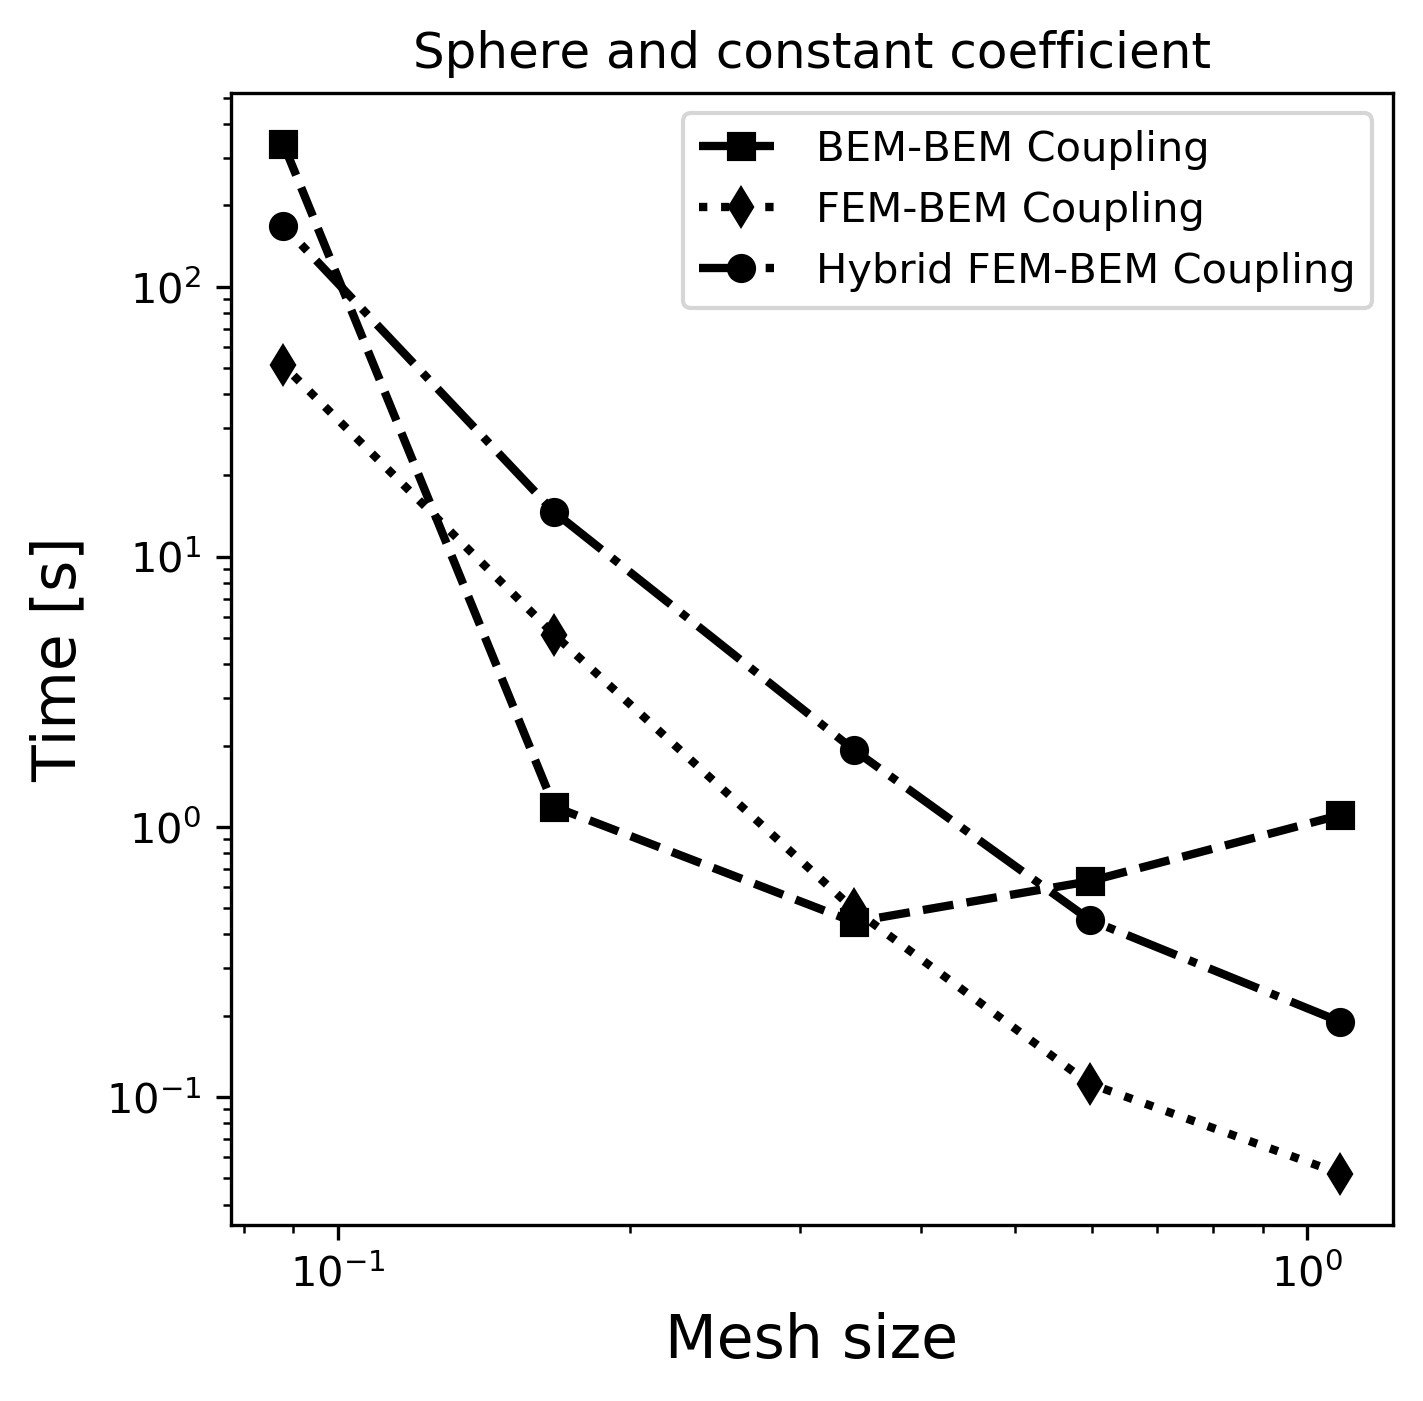
\includegraphics[width=0.45\linewidth]{Sphere_const_coeff_time.png}
  \caption{Error for the Kirkwood sphere.}
  \label{fig:error_sphere}
\end{figure}

%\begin{itemize}
%    \item Show convergence to analytical solution for
%    \begin{itemize}
%        \item BEM-BEM
%\begin{figure}[!htb]
%\minipage{0.32\textwidth}
%  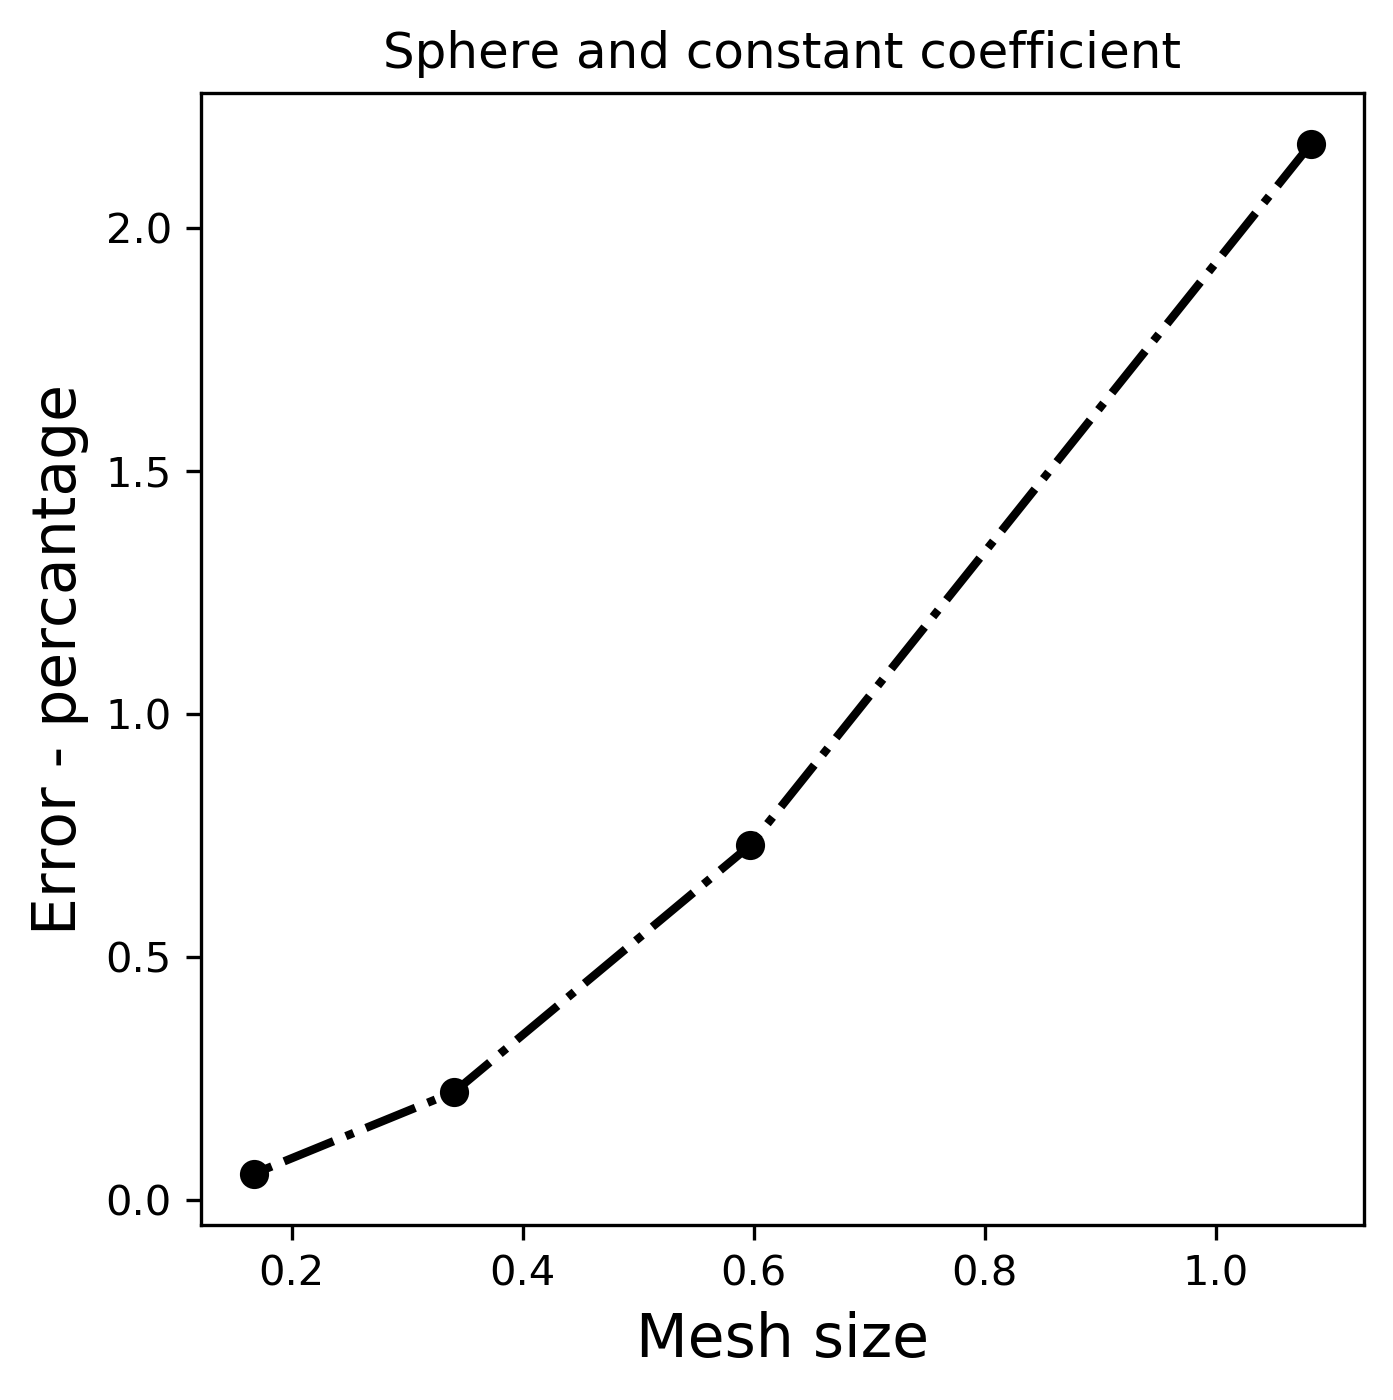
\includegraphics[width=\linewidth]{BEM_BEM_Sphere_const_coeff_error.png}
%  \caption{Error}
%\endminipage\hfill
%\minipage{0.32\textwidth}
%  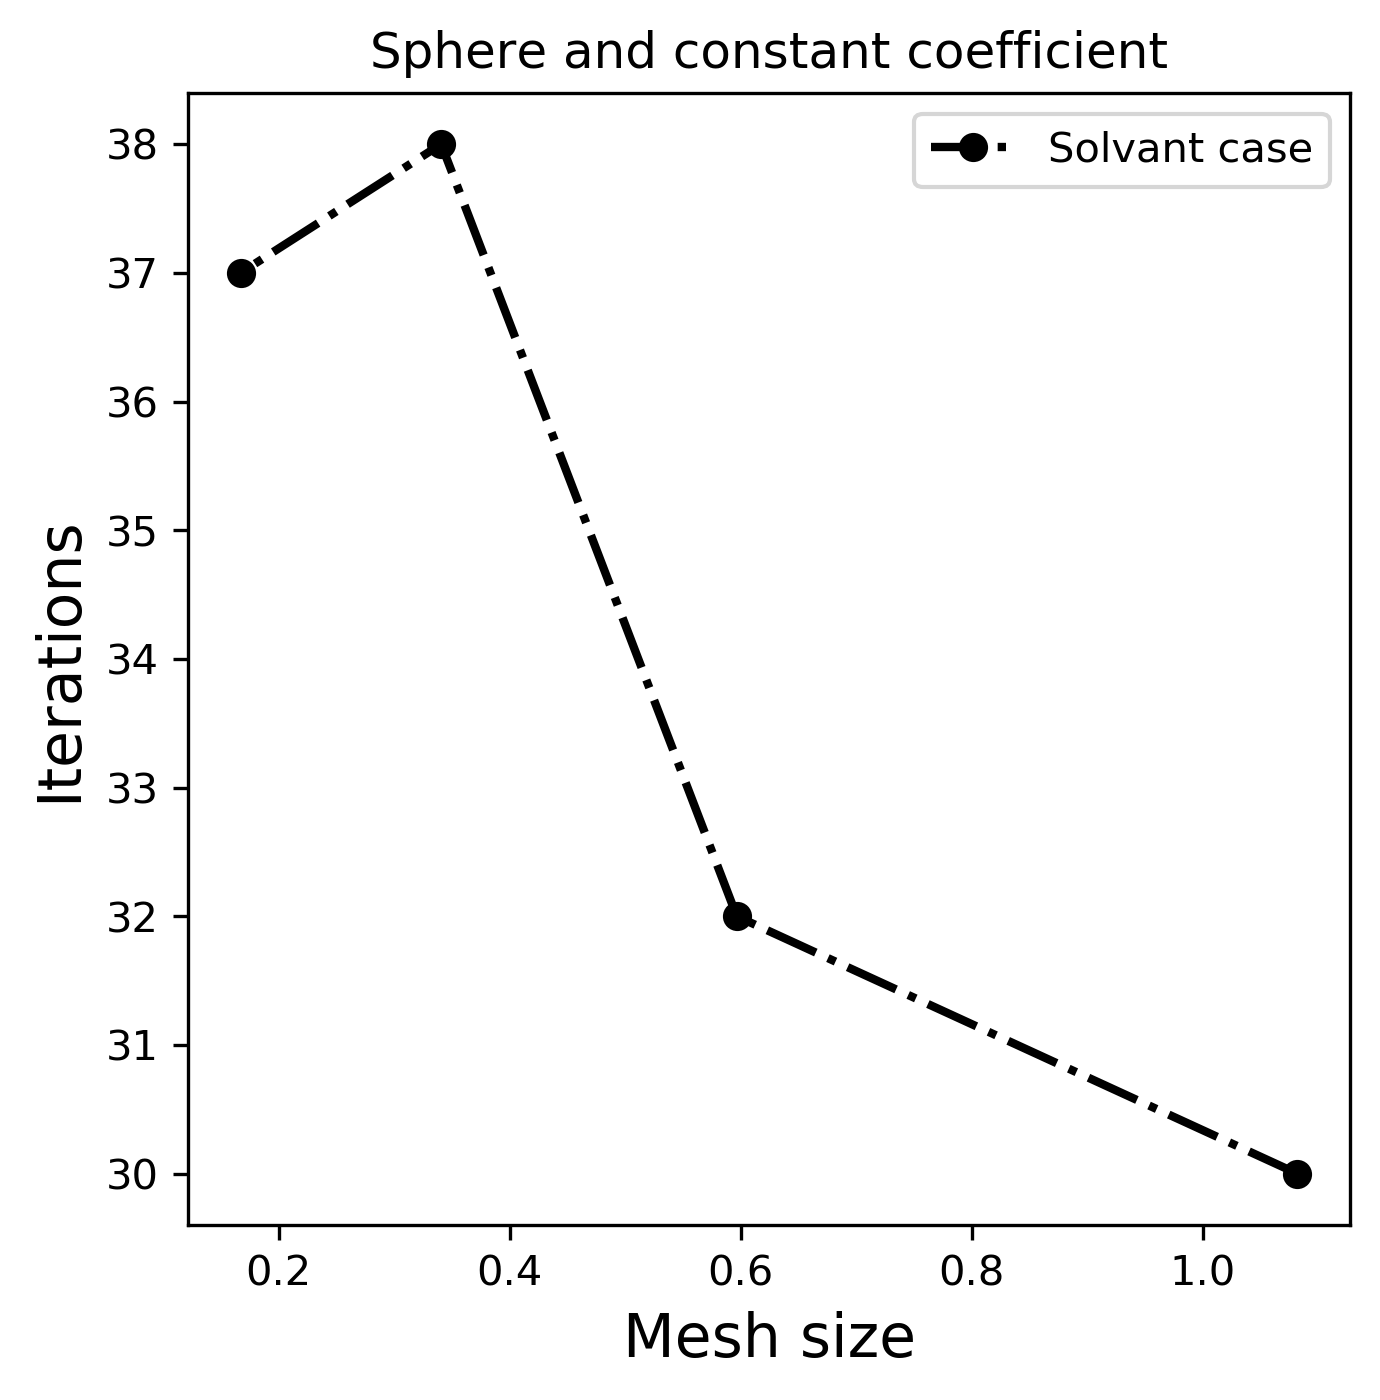
\includegraphics[width=\linewidth]{BEM_BEM_Sphere_const_coeff_iter.png}
%  \caption{Iterations}
%\endminipage\hfill
%\minipage{0.32\textwidth}%
%  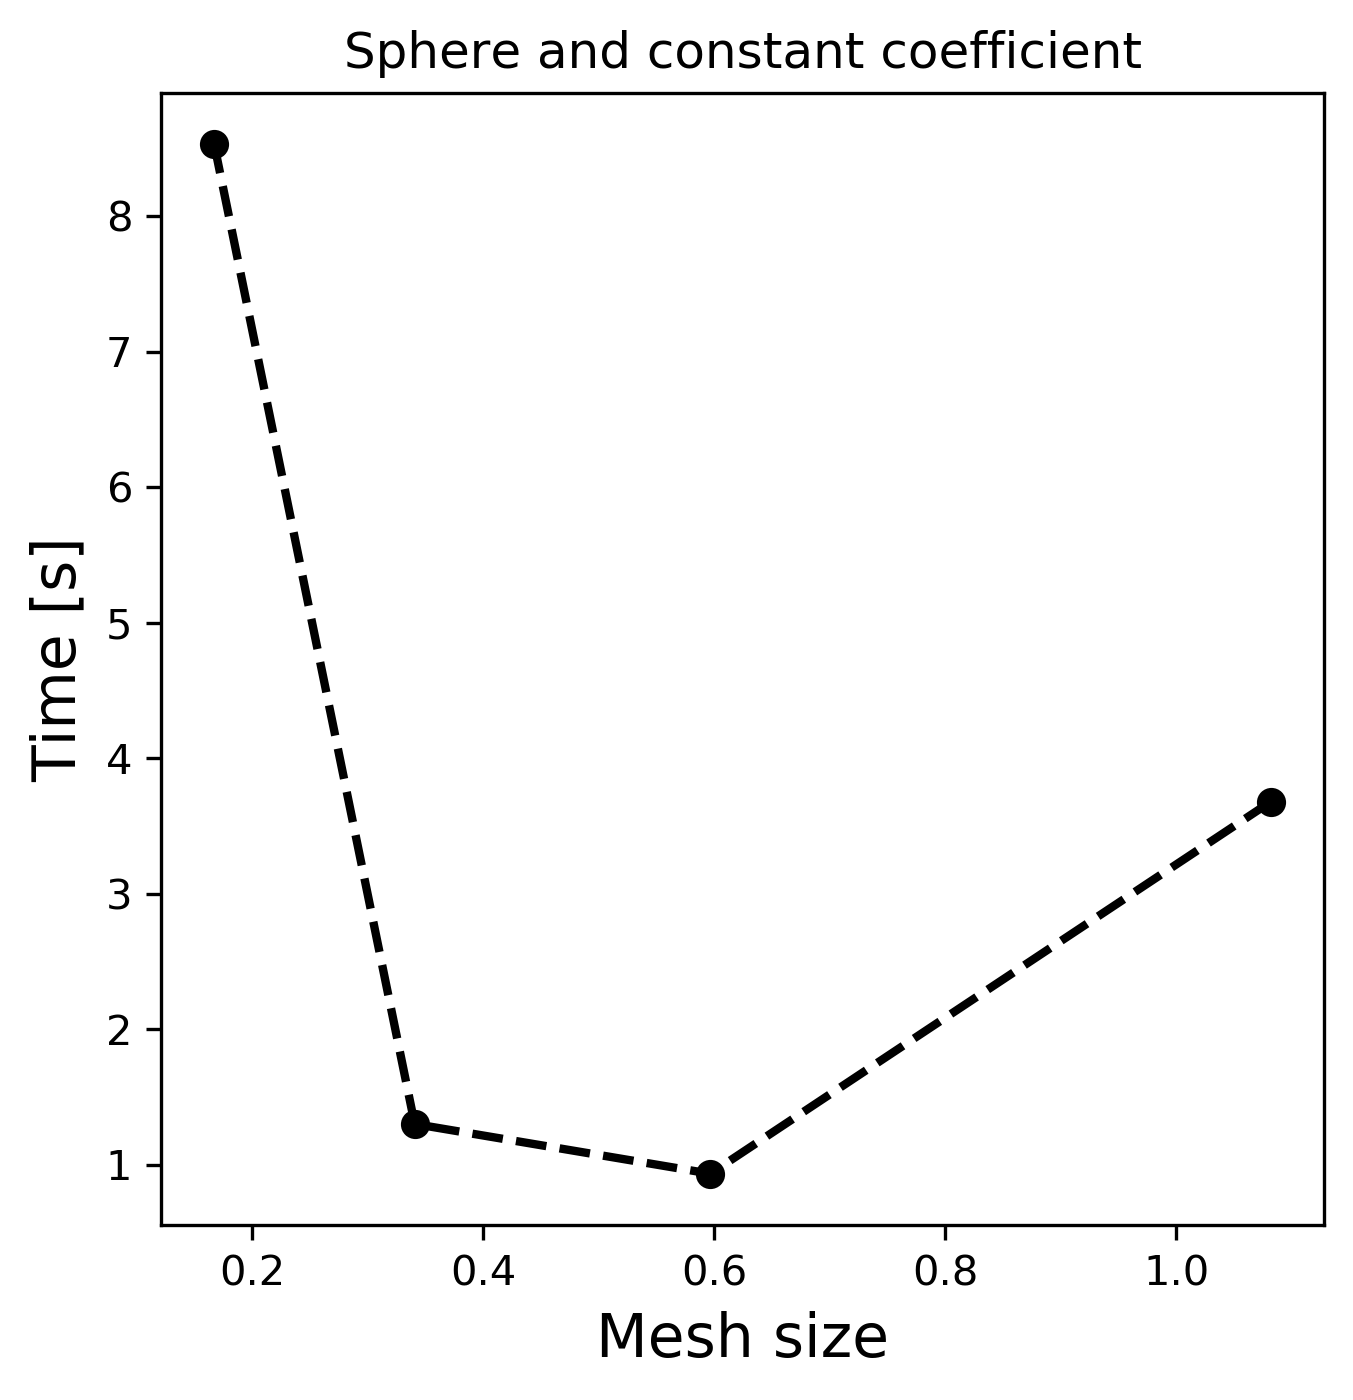
\includegraphics[width=\linewidth]{BEM_BEM_Sphere_const_coeff_time.png}
%  \caption{Computational time}
%\endminipage
%\end{figure}
%        \item Standard FEM-BEM
%\begin{figure}[!htb]
%\minipage{0.32\textwidth}
%  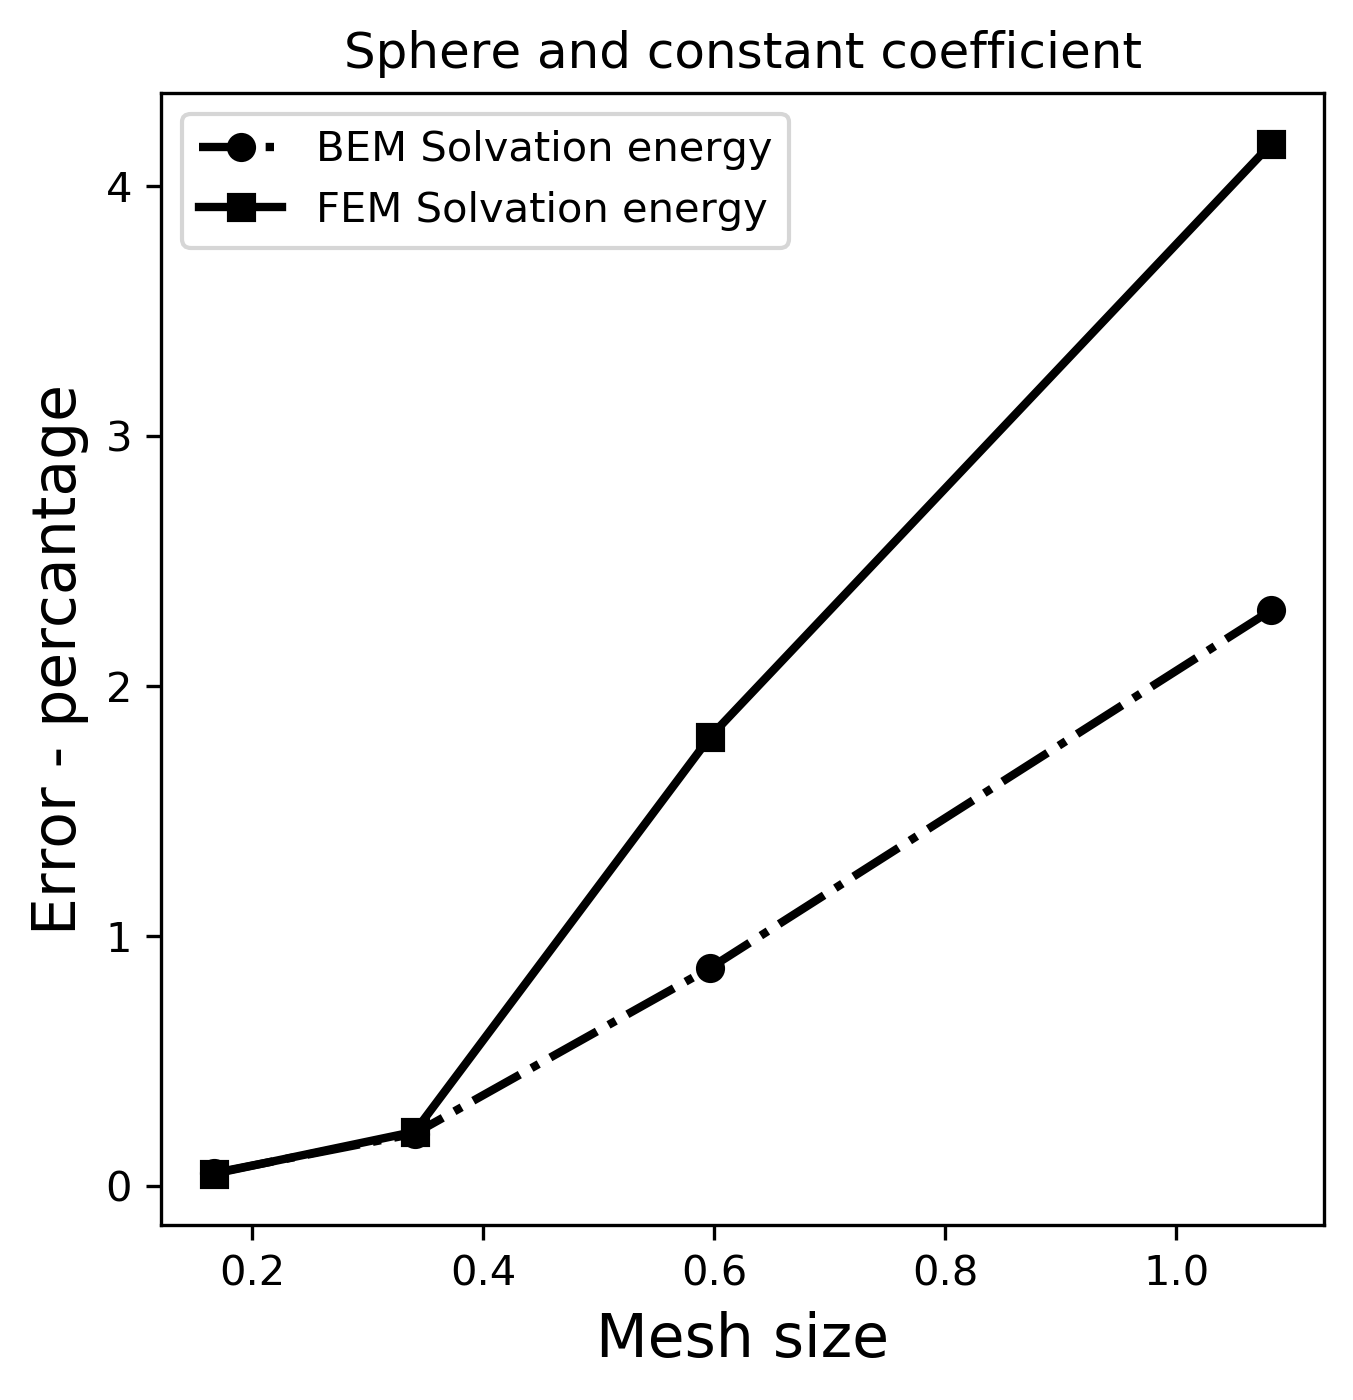
\includegraphics[width=\linewidth]{FEM_BEM_Sphere_const_coeff_error.png}
%  \caption{Error}
%\endminipage\hfill
%\minipage{0.32\textwidth}
%  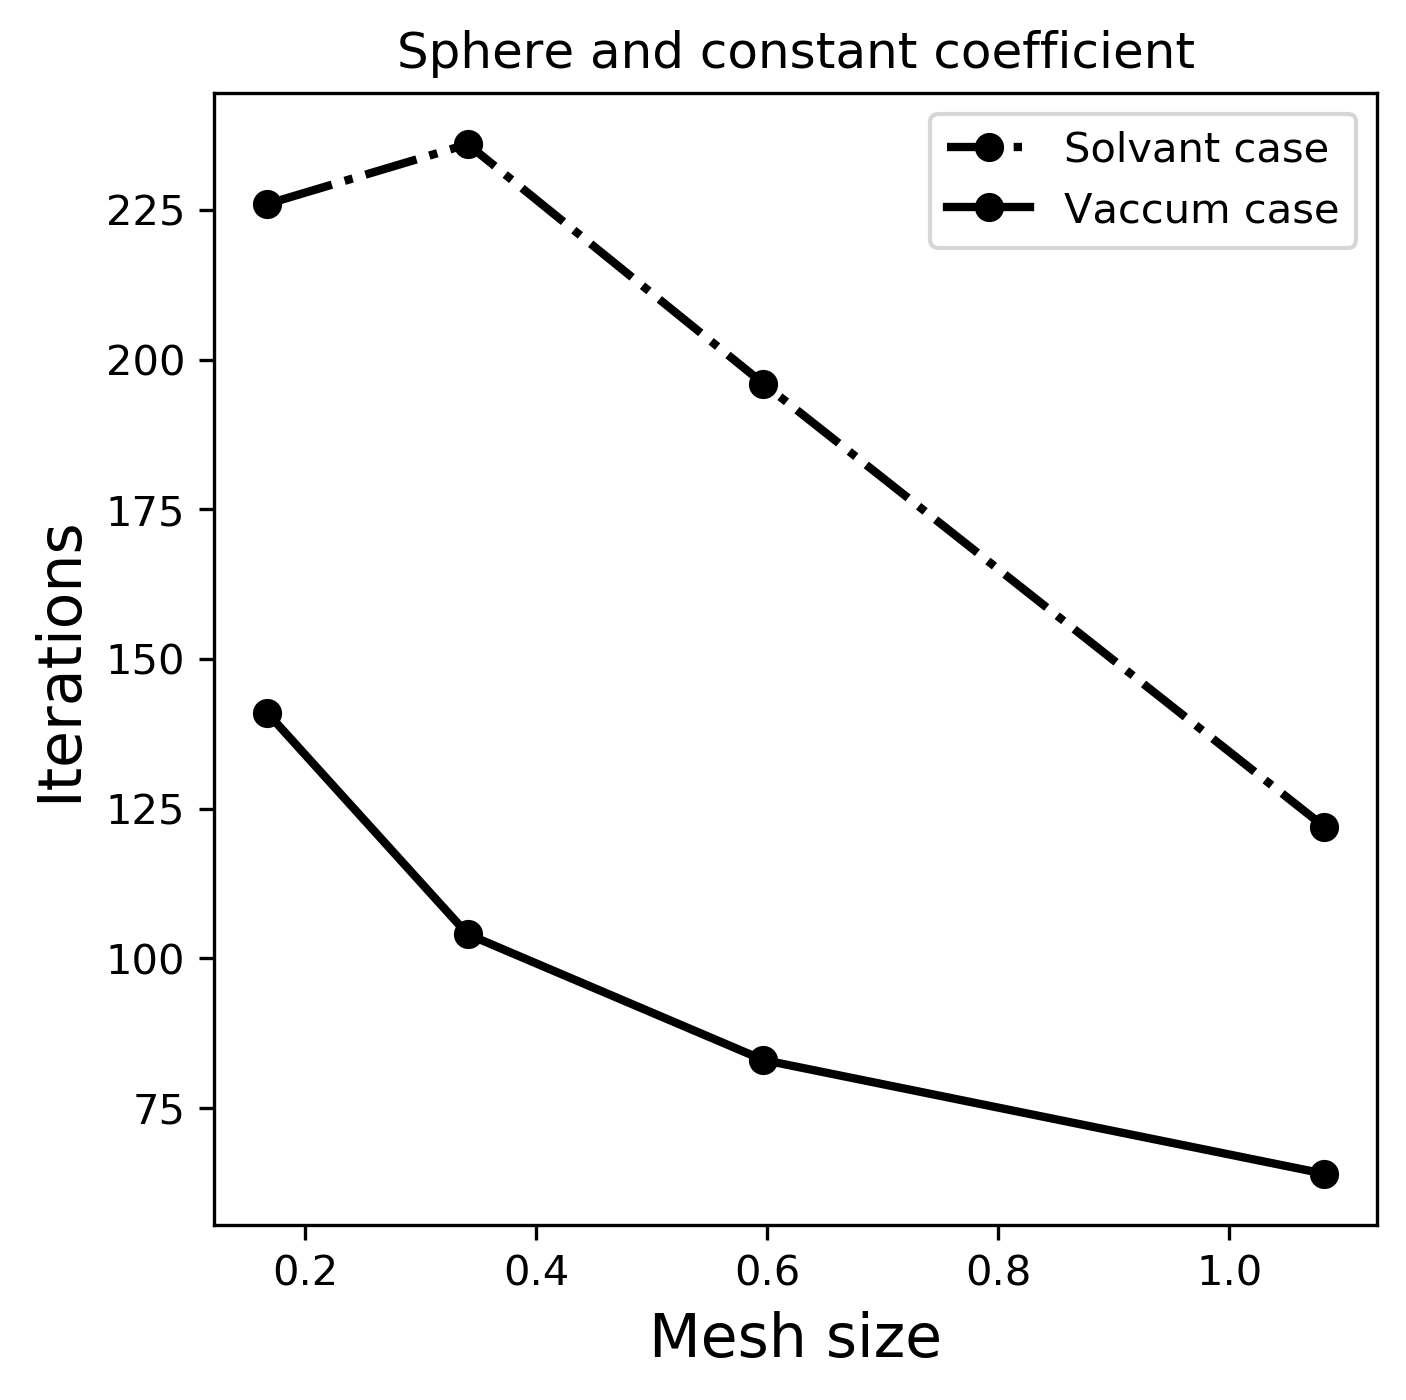
\includegraphics[width=\linewidth]{FEM_BEM_Sphere_const_coeff_iter.png}
%  \caption{Iterations}
%\endminipage\hfill
%\minipage{0.32\textwidth}%
%  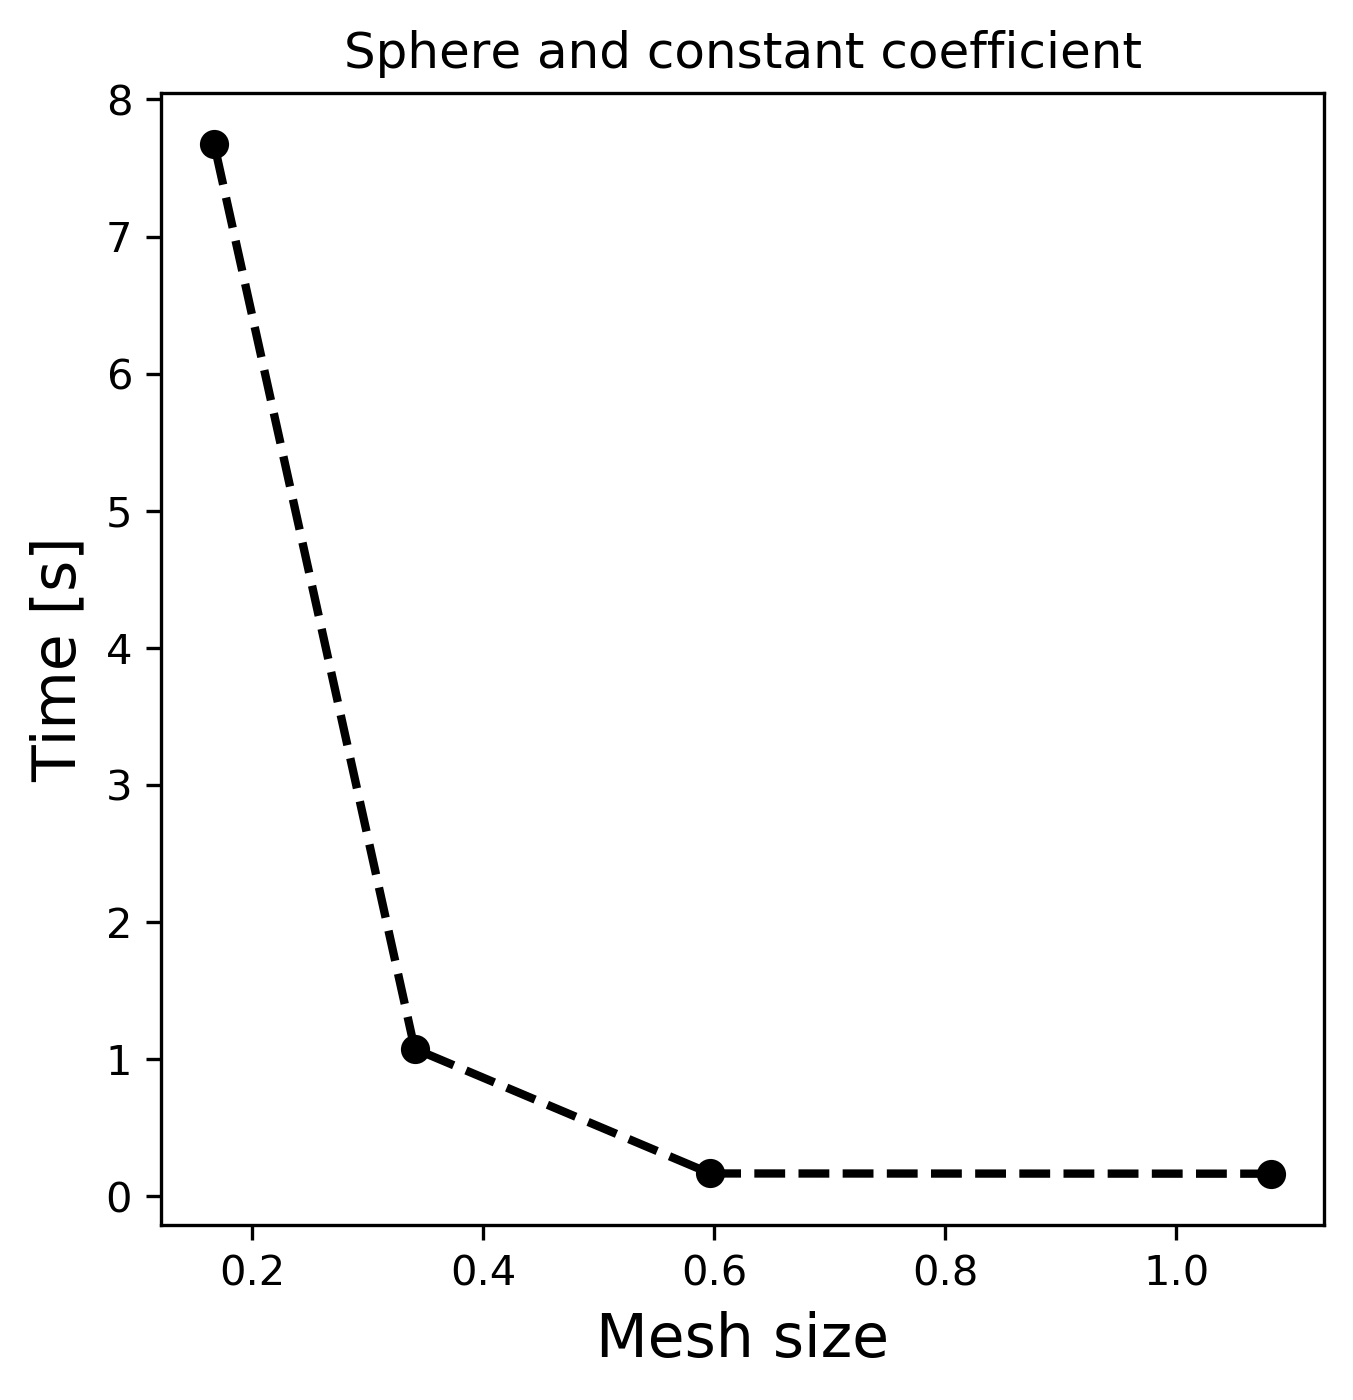
\includegraphics[width=\linewidth]{FEM_BEM_Sphere_const_coeff_time.png}
%  \caption{Computational time}
%\endminipage
%\end{figure}
%        \item Hybrid FEM-BEM
%\begin{figure}[!htb]
%\minipage{0.32\textwidth}
%  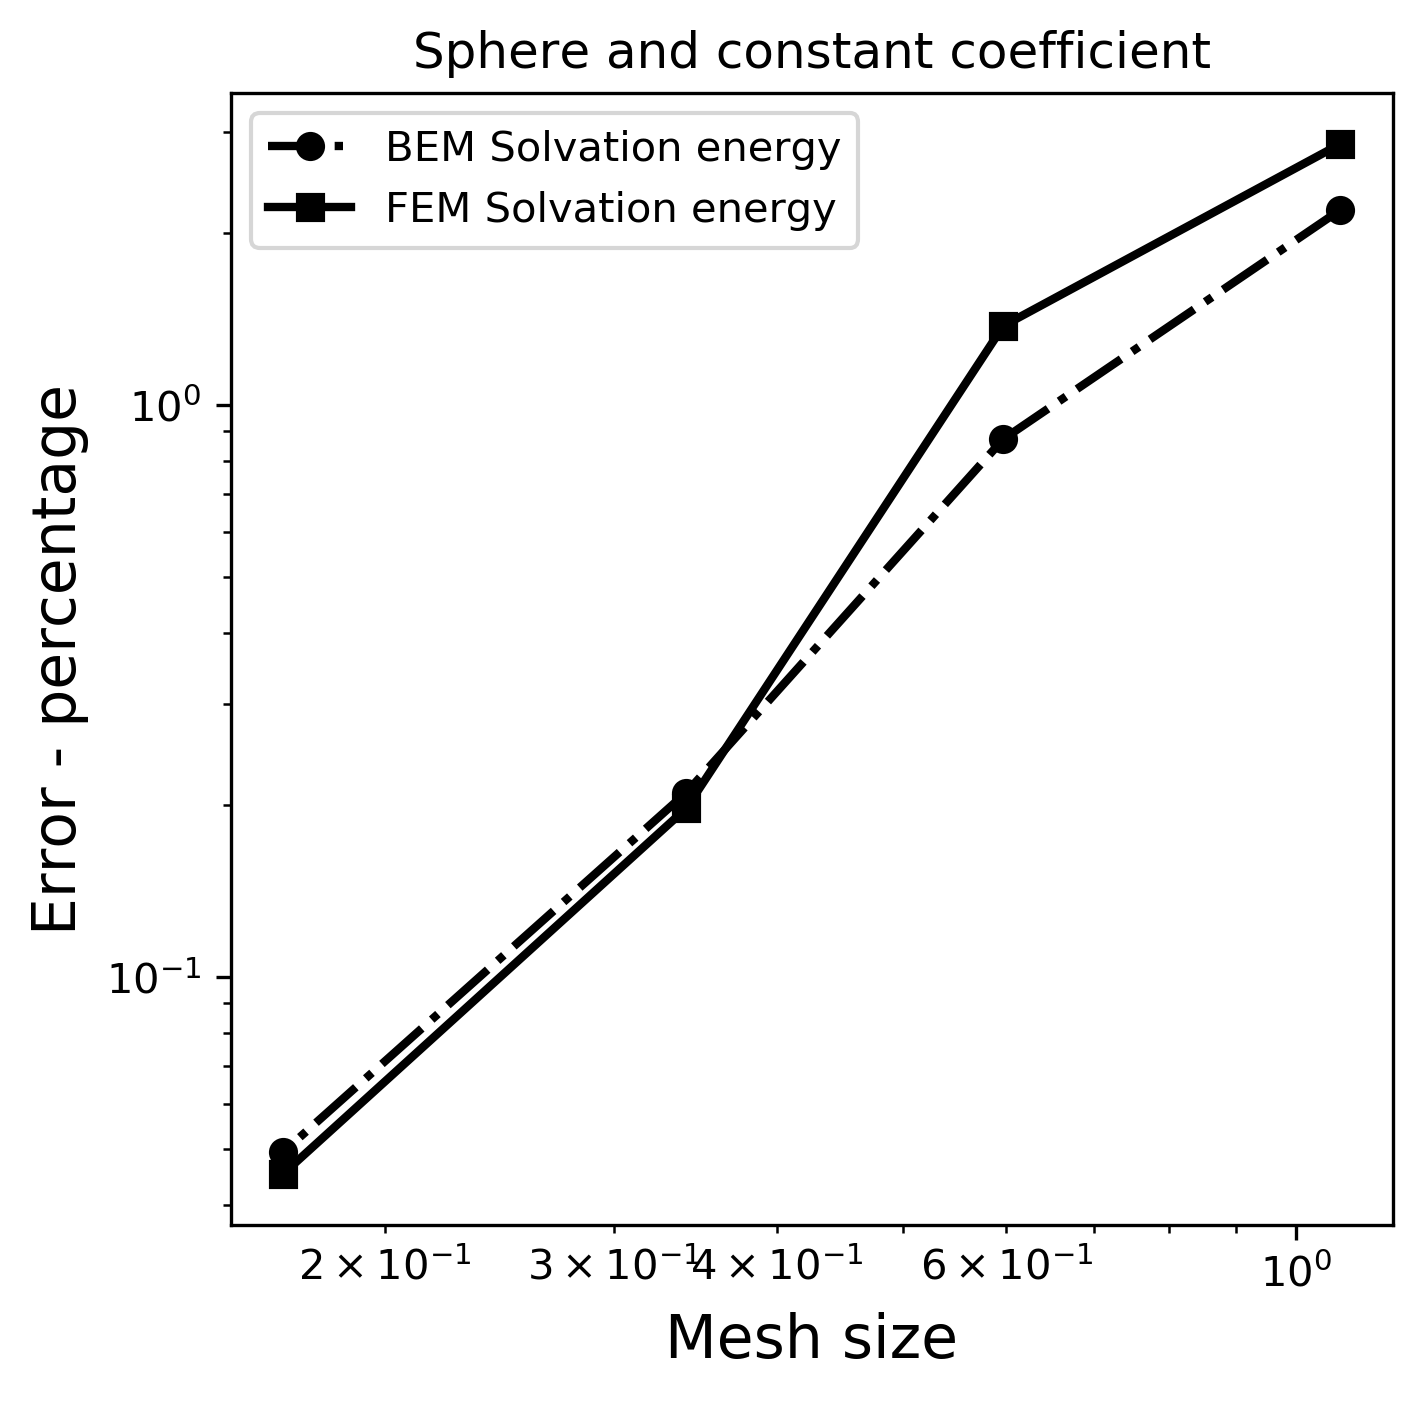
\includegraphics[width=\linewidth]{Hybrid_FEM_BEM_Sphere_const_coeff_error.png}
%  \caption{Error}
%\endminipage\hfill
%\minipage{0.32\textwidth}
%  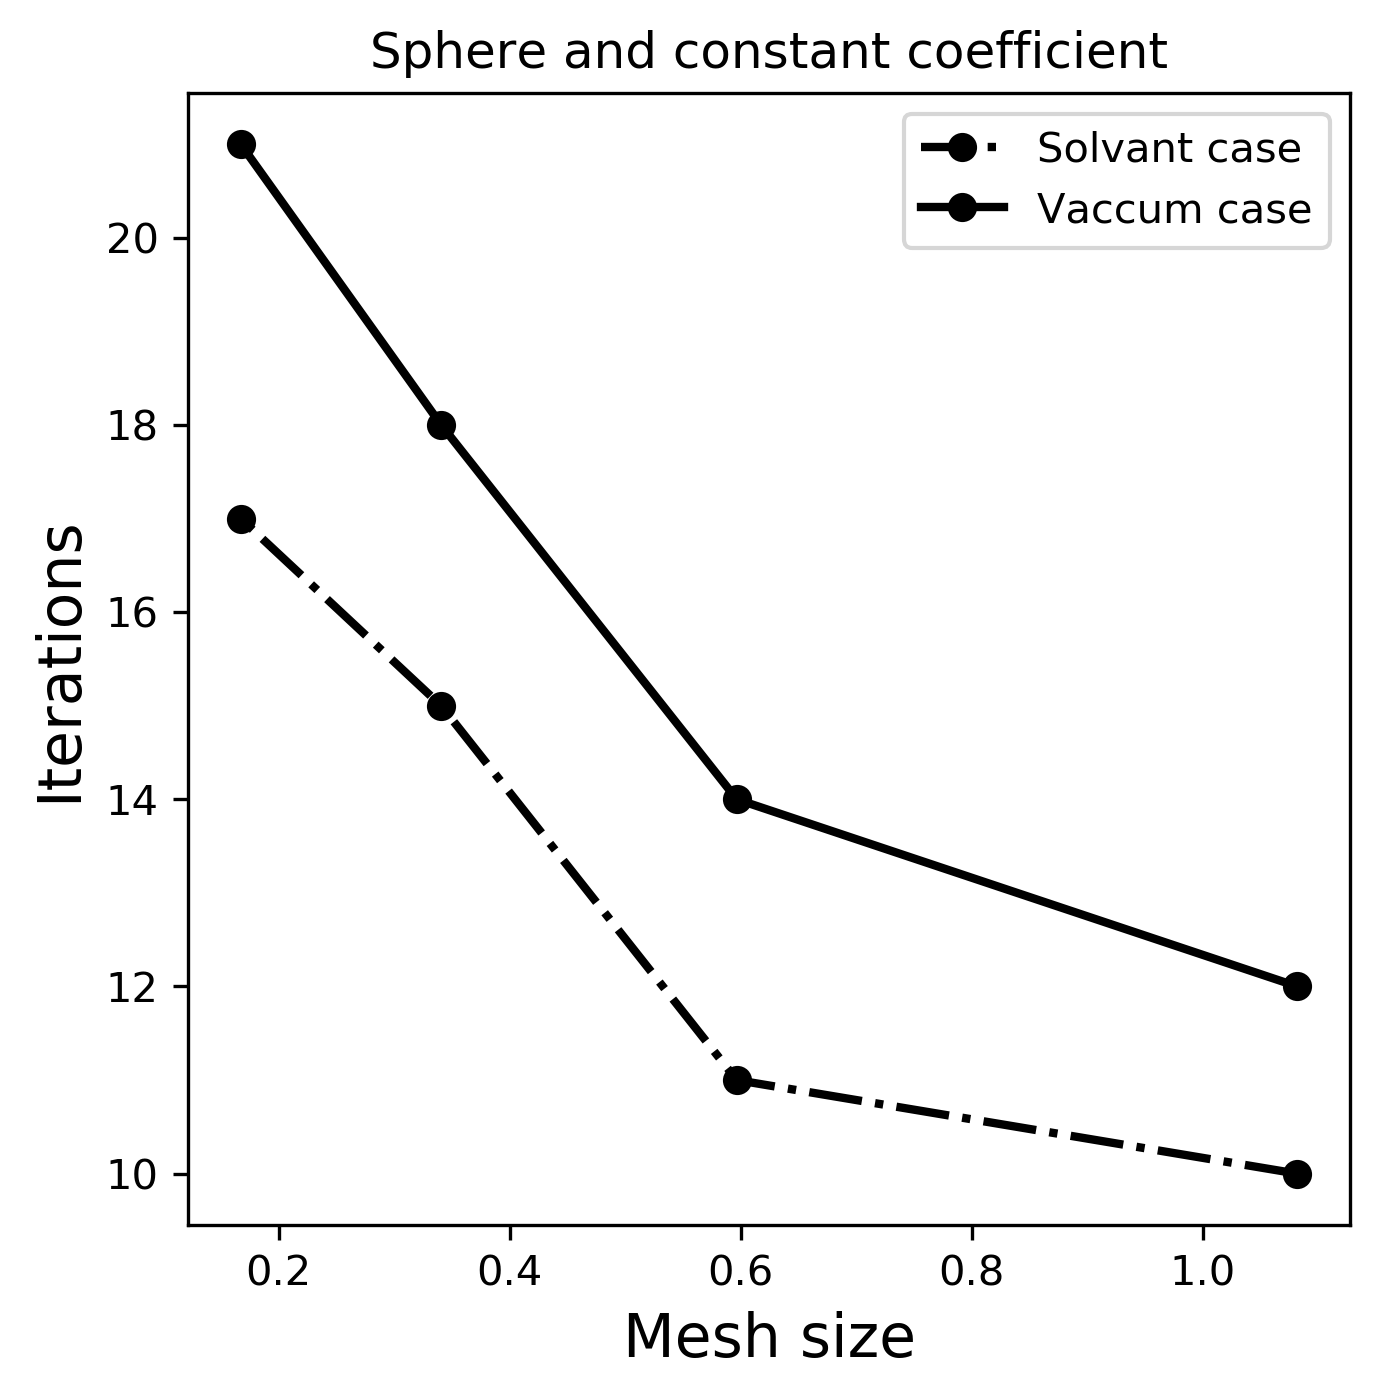
\includegraphics[width=\linewidth]{Hybrid_FEM_BEM_Sphere_const_coeff_iter.png}
%  \caption{Iterations}
%\endminipage\hfill
%\minipage{0.32\textwidth}%
%  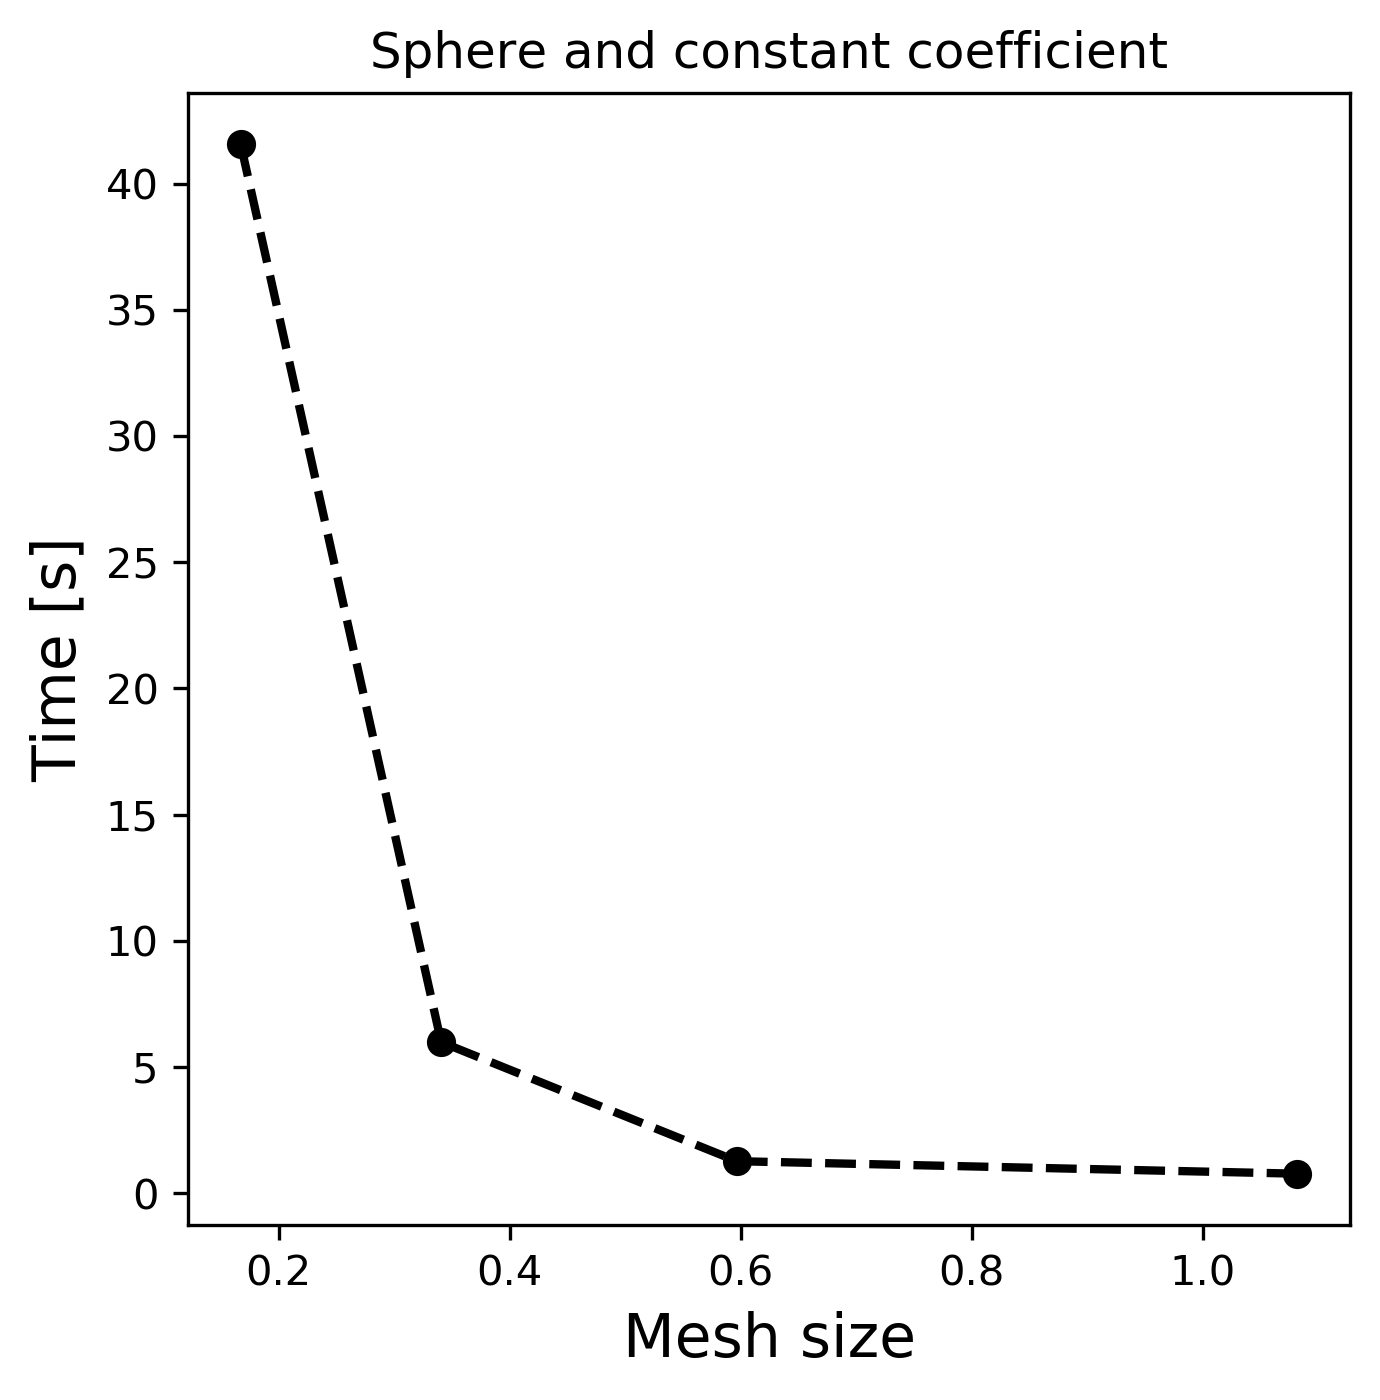
\includegraphics[width=\linewidth]{Hybrid_FEM_BEM_Sphere_const_coeff_time.png}
%  \caption{Computational time}
%\endminipage
%\end{figure}
%    \end{itemize}
%\end{itemize}

\subsection*{\sffamily \large Performance for arginine}

As a more realistic test, we assessed the performance of the standard and hybrid FEM-BEM coupling techniques against a purely BEM implementation for arginine [cite arg]. 
We generated surface meshes containing W, X, Y, and Z vertices per \AA$^2$ with Nanoshaper [Rocchia].
These meshes were inputs to our purely BEM solver, and to create the FEM mesh with pyGAMer [pygamer], invoking \texttt{tetgen} with the string \texttt{abcd}.
For the hybrid FEM-BEM coupling approach, we used $\tau$=10.

Figure \ref{fig:arg_constant_time} compares the time-to-solution with the three schemes, and shows that using only BEM outperforms both coupled FEM-BEM approaches.
Even though hybrid FEM-BEM is slower than standard FEM-BEM in Figure \ref{fig:arg_constant_time}, the iteration count in Figure \ref{fig:arg_constant_iter} shows that hybrid FEM-BEM needs less iterations (can we compare them?). 
This behavior is promising going towards larger problems, specially since the hybrid approach allows for more flexibility in the choice of preconditioner.
We can also see that accuracy is not affected (or is?) by considering a FEM region inside the molecule (need fig to check this).

Do we really need to compute the vacuum case numerically? We should be able to do it analytically, right?

\begin{figure}
\centering
%   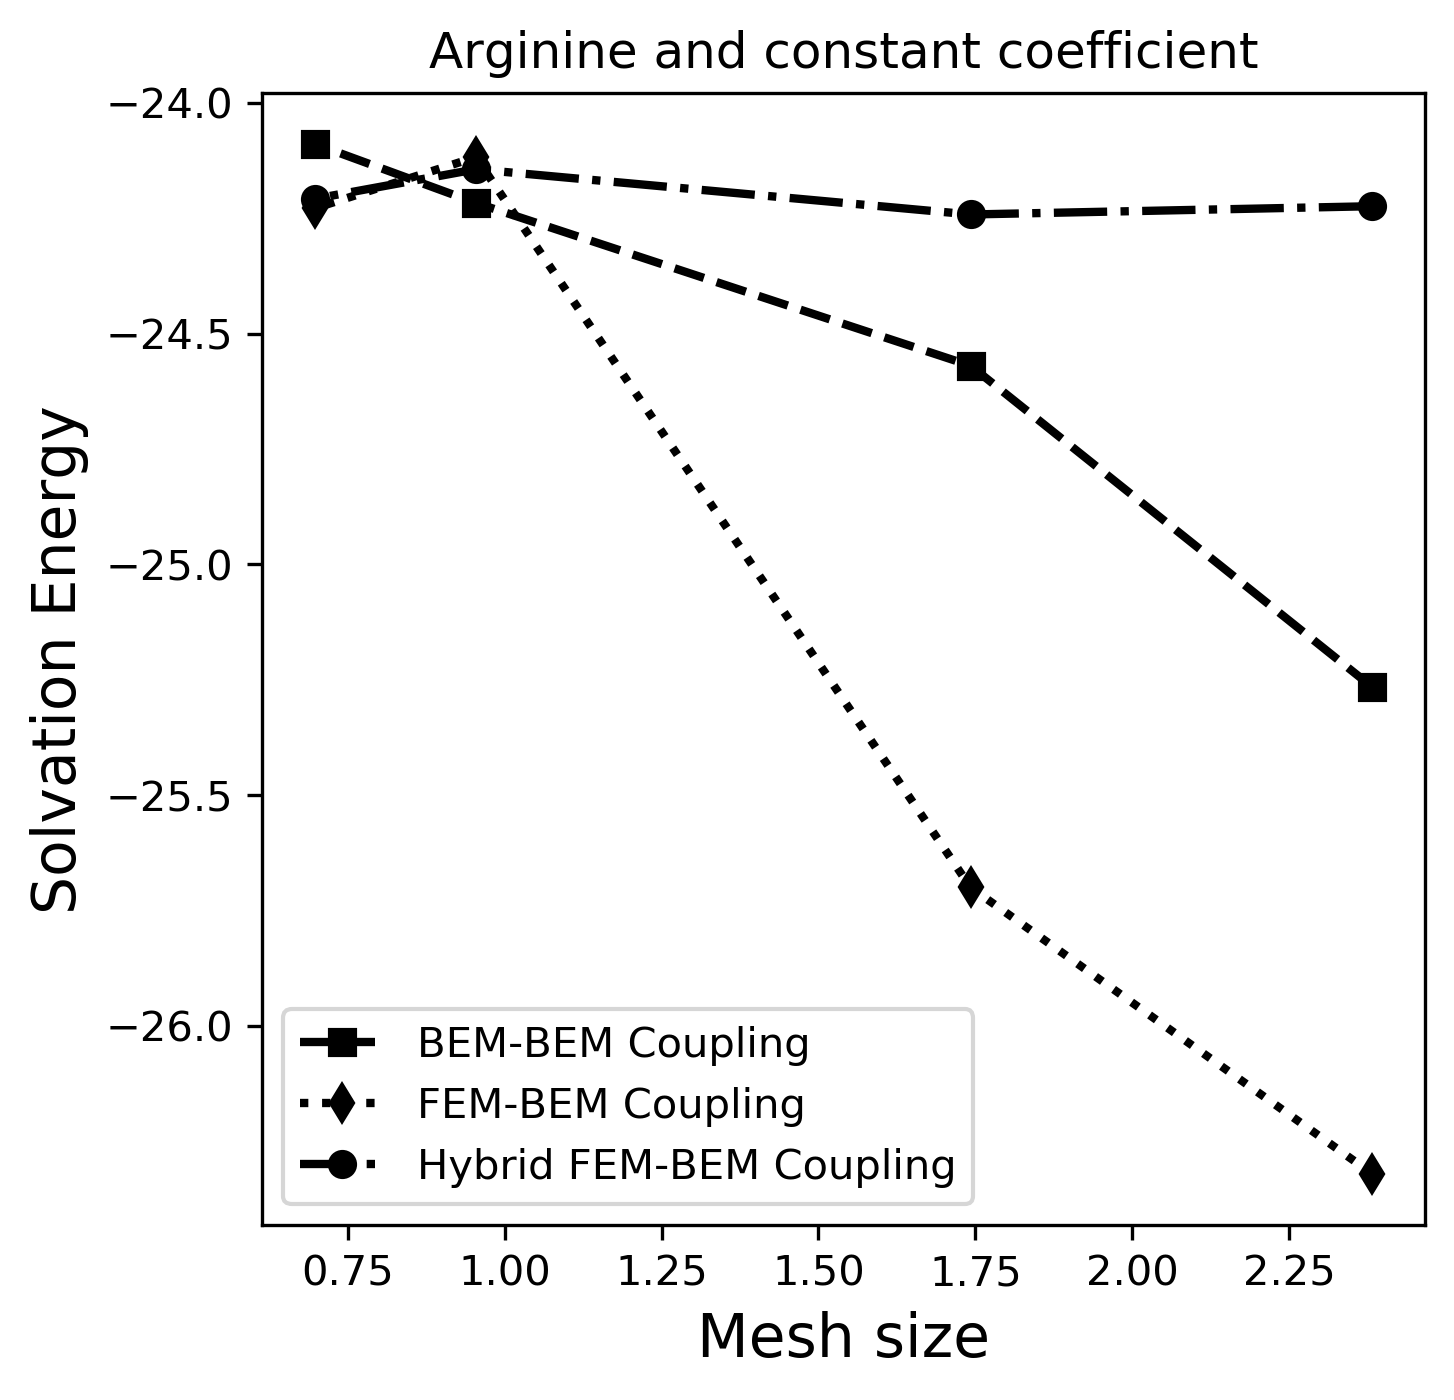
\includegraphics[width=0.45\linewidth]{Arginine_const_coeff_error.png}
%   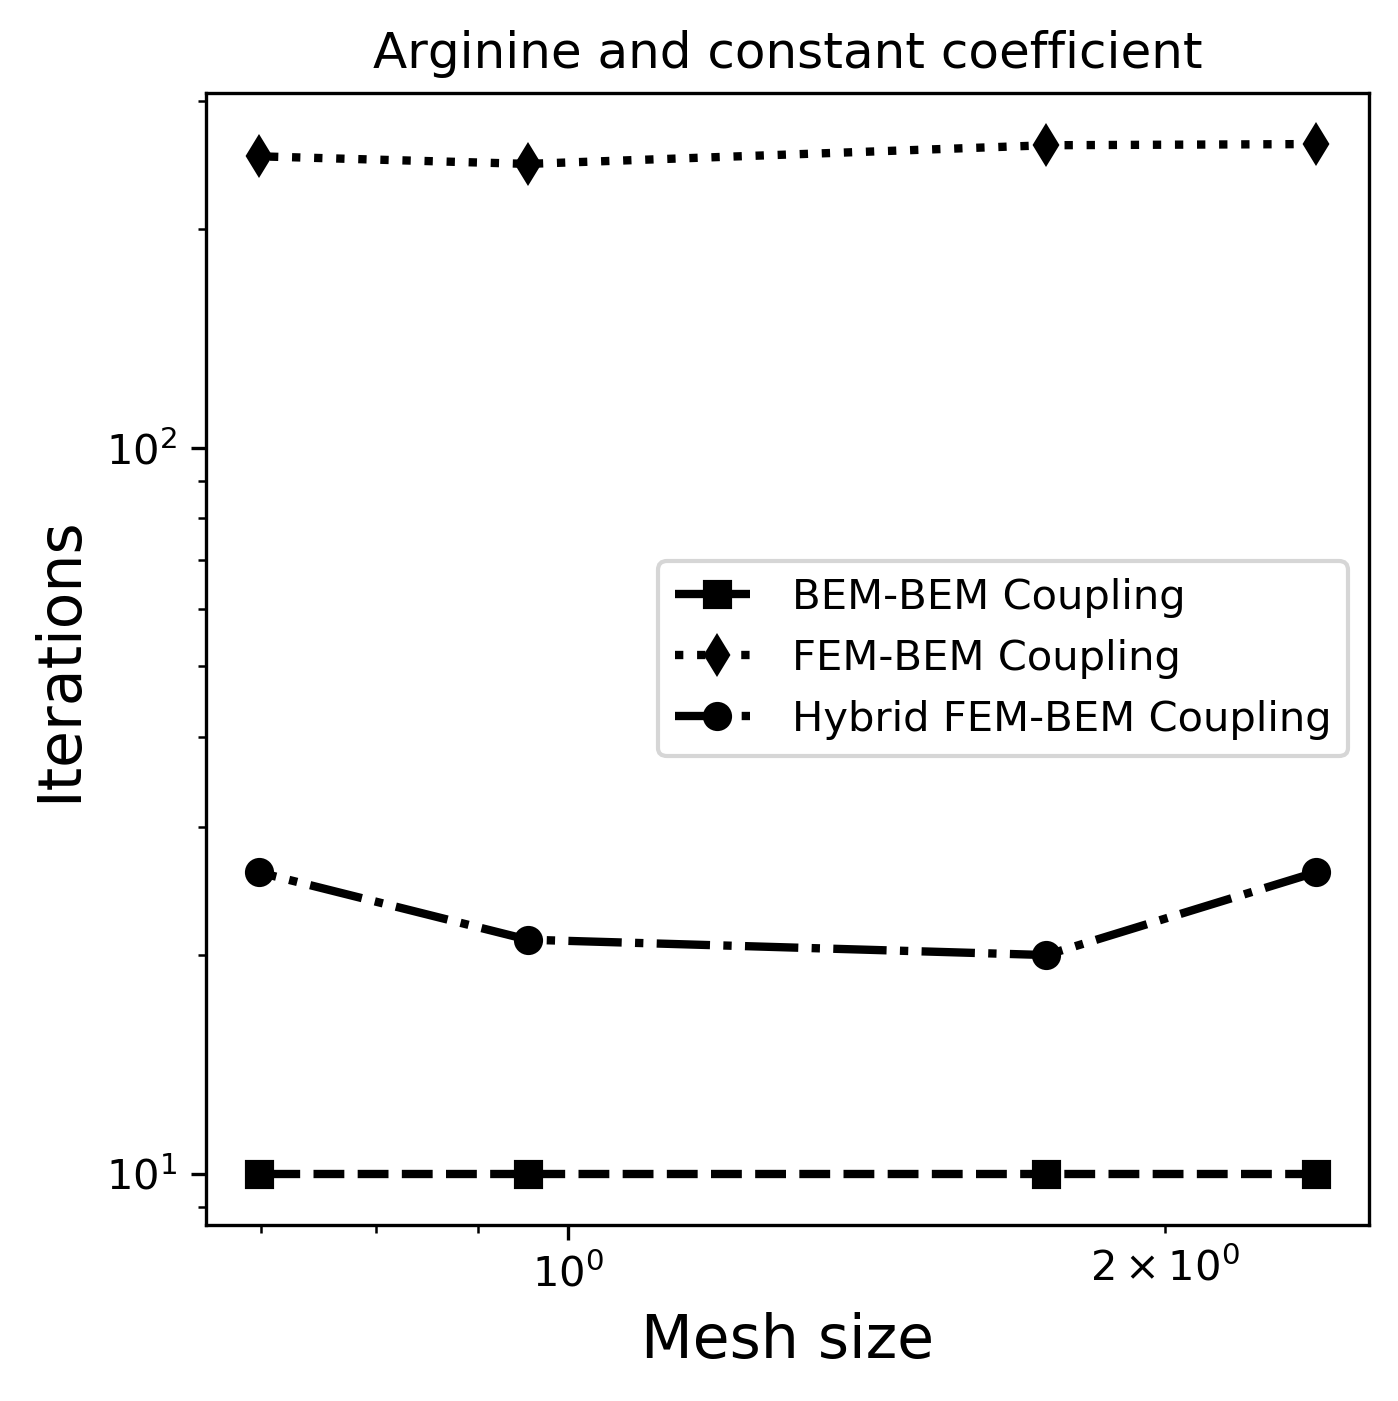
\includegraphics[width=0.45\linewidth]{Arginine_const_coeff_iter.png}
  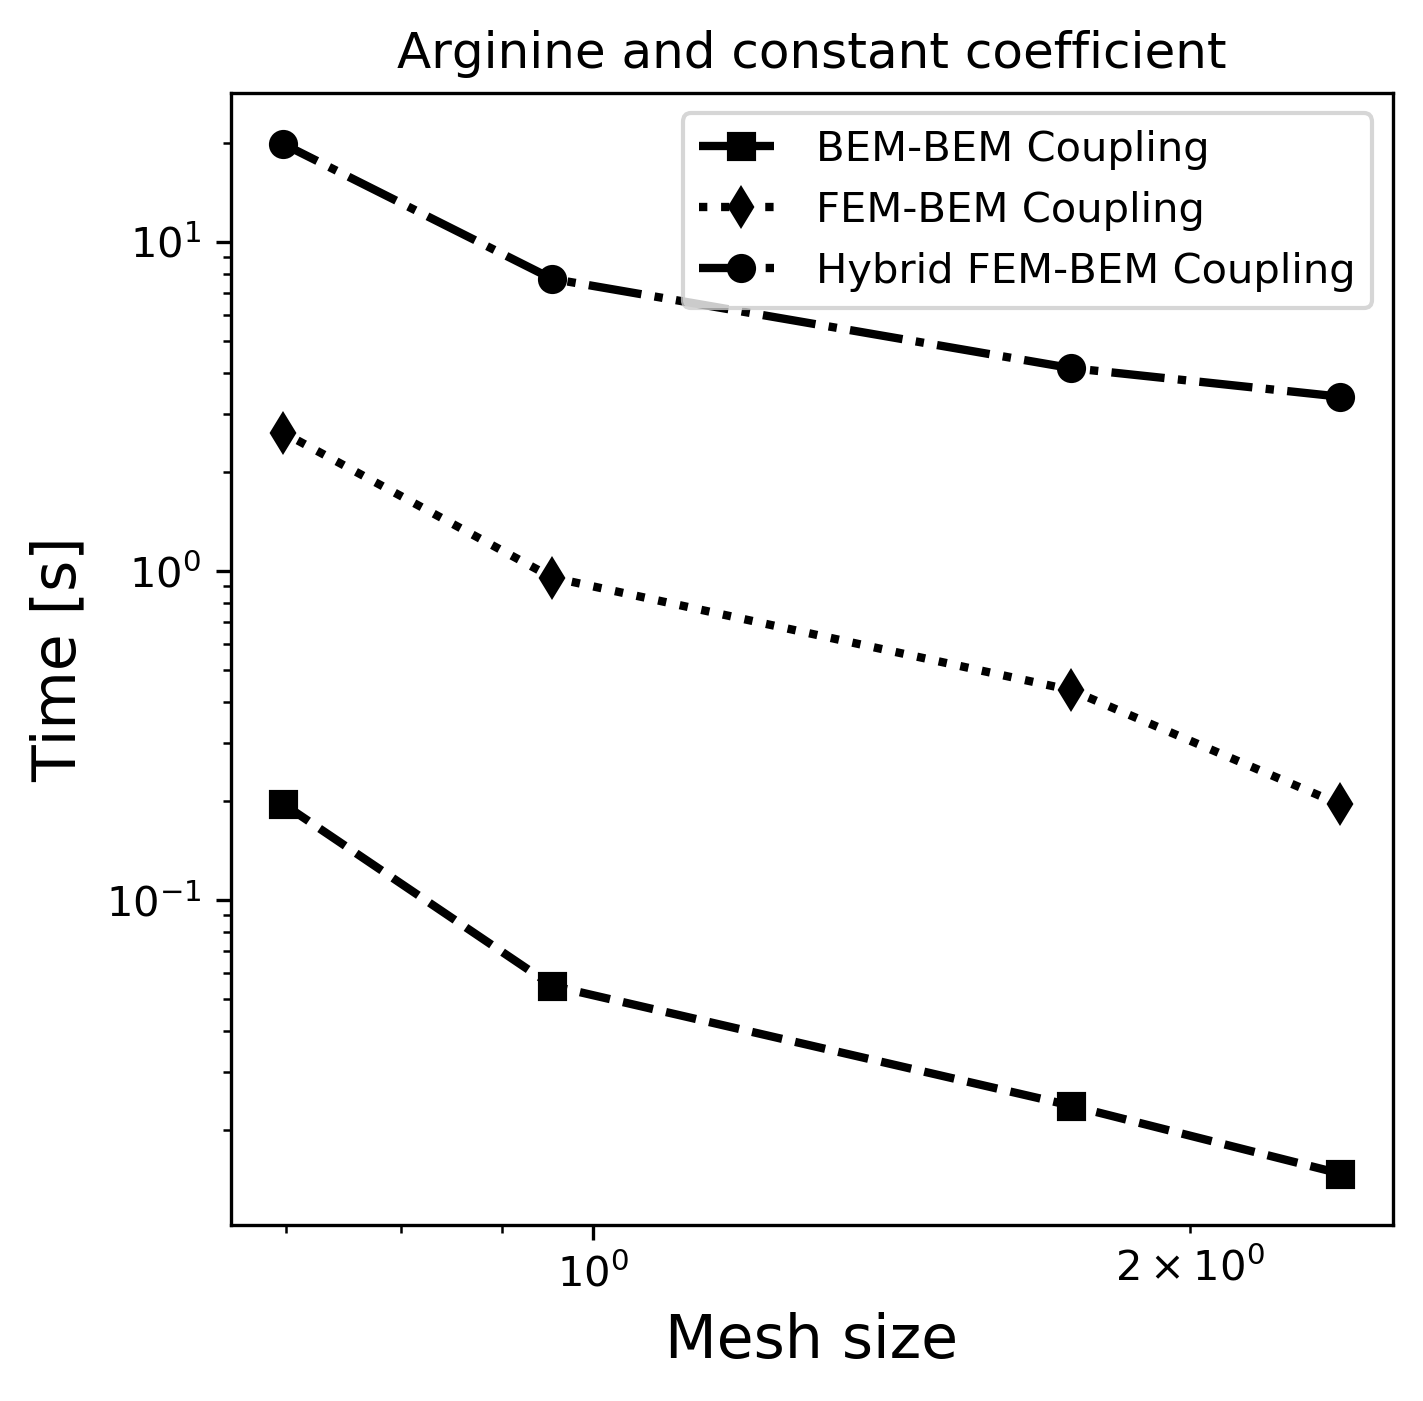
\includegraphics[width=0.6\linewidth]{Arginine_const_coeff_time.png}
\caption{Time-to-solution for arginine with a constant permittivity. %(1) fix title, (2) can we put them in a single plot, (3) 
maybe we could also add a "error" wrt extrapolation, or a plot with energy for each mesh?}
\label{fig:arg_contant_time}
\end{figure}


\begin{figure}
\centering
%   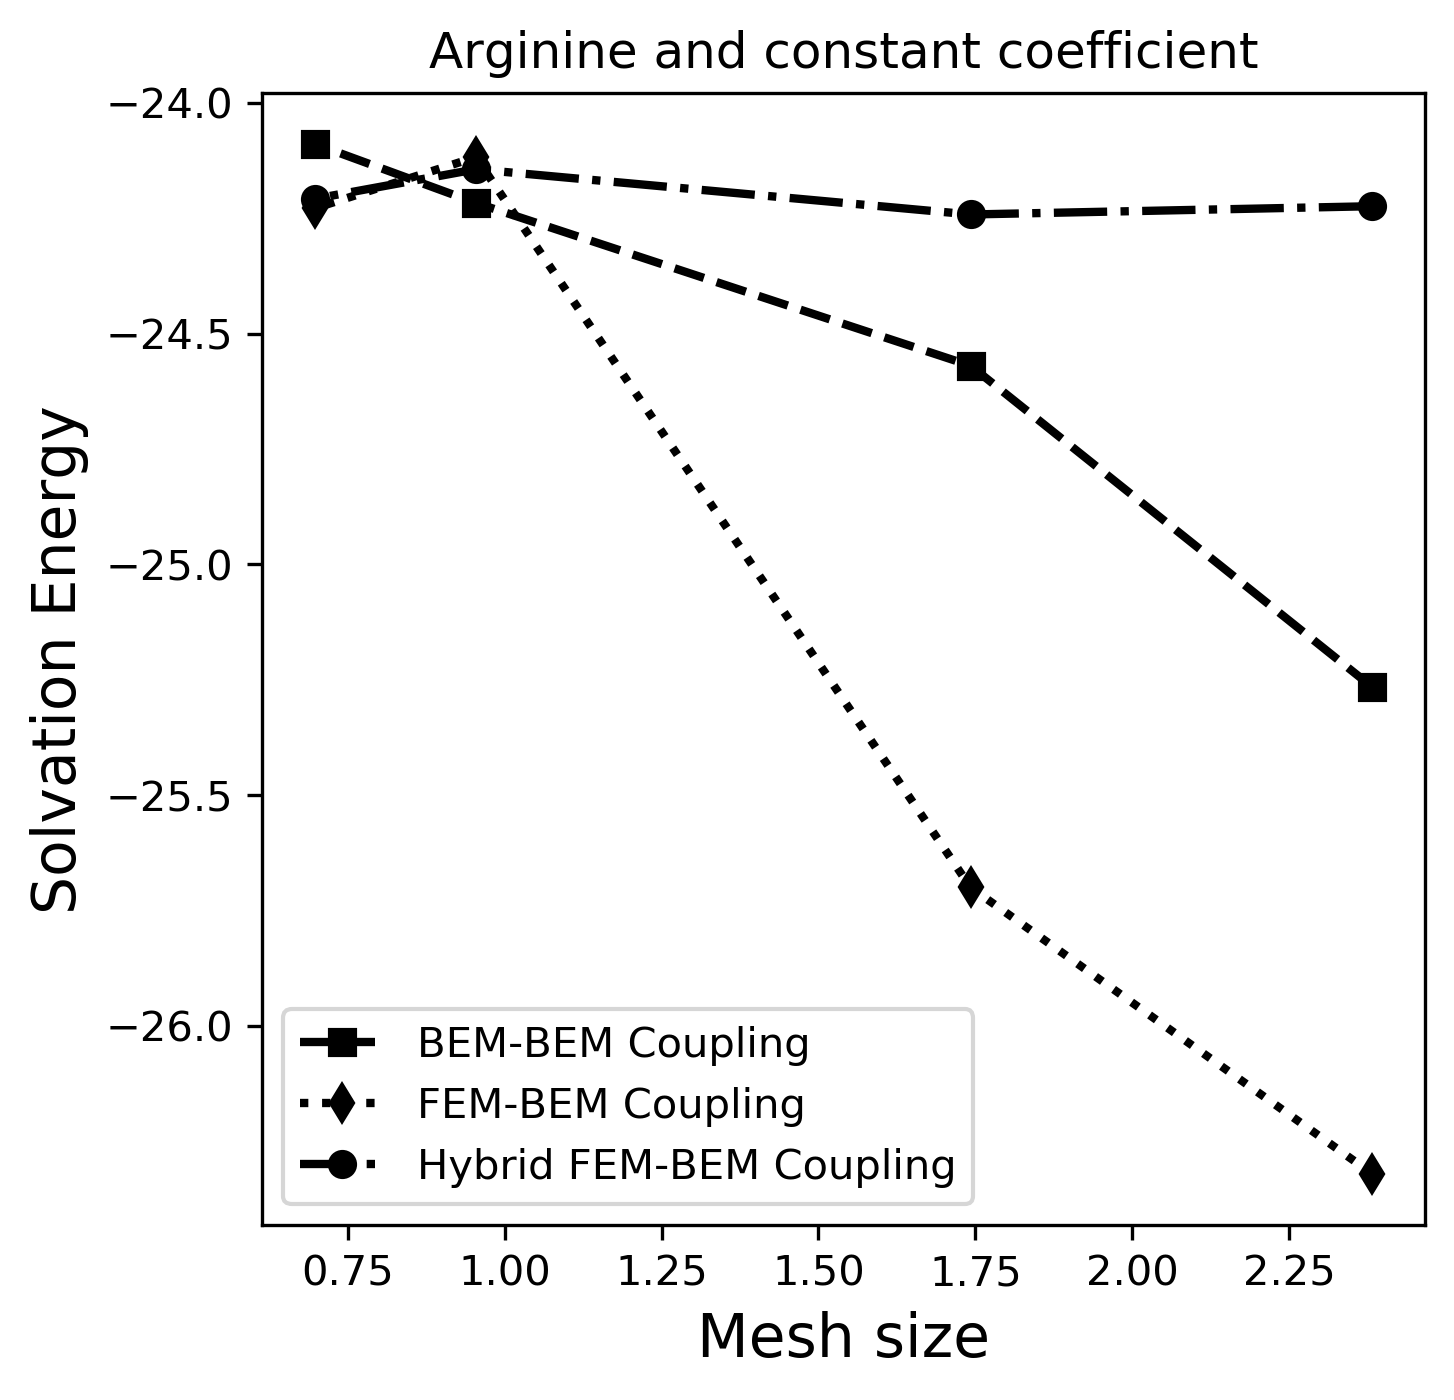
\includegraphics[width=0.45\linewidth]{Arginine_const_coeff_error.png}
  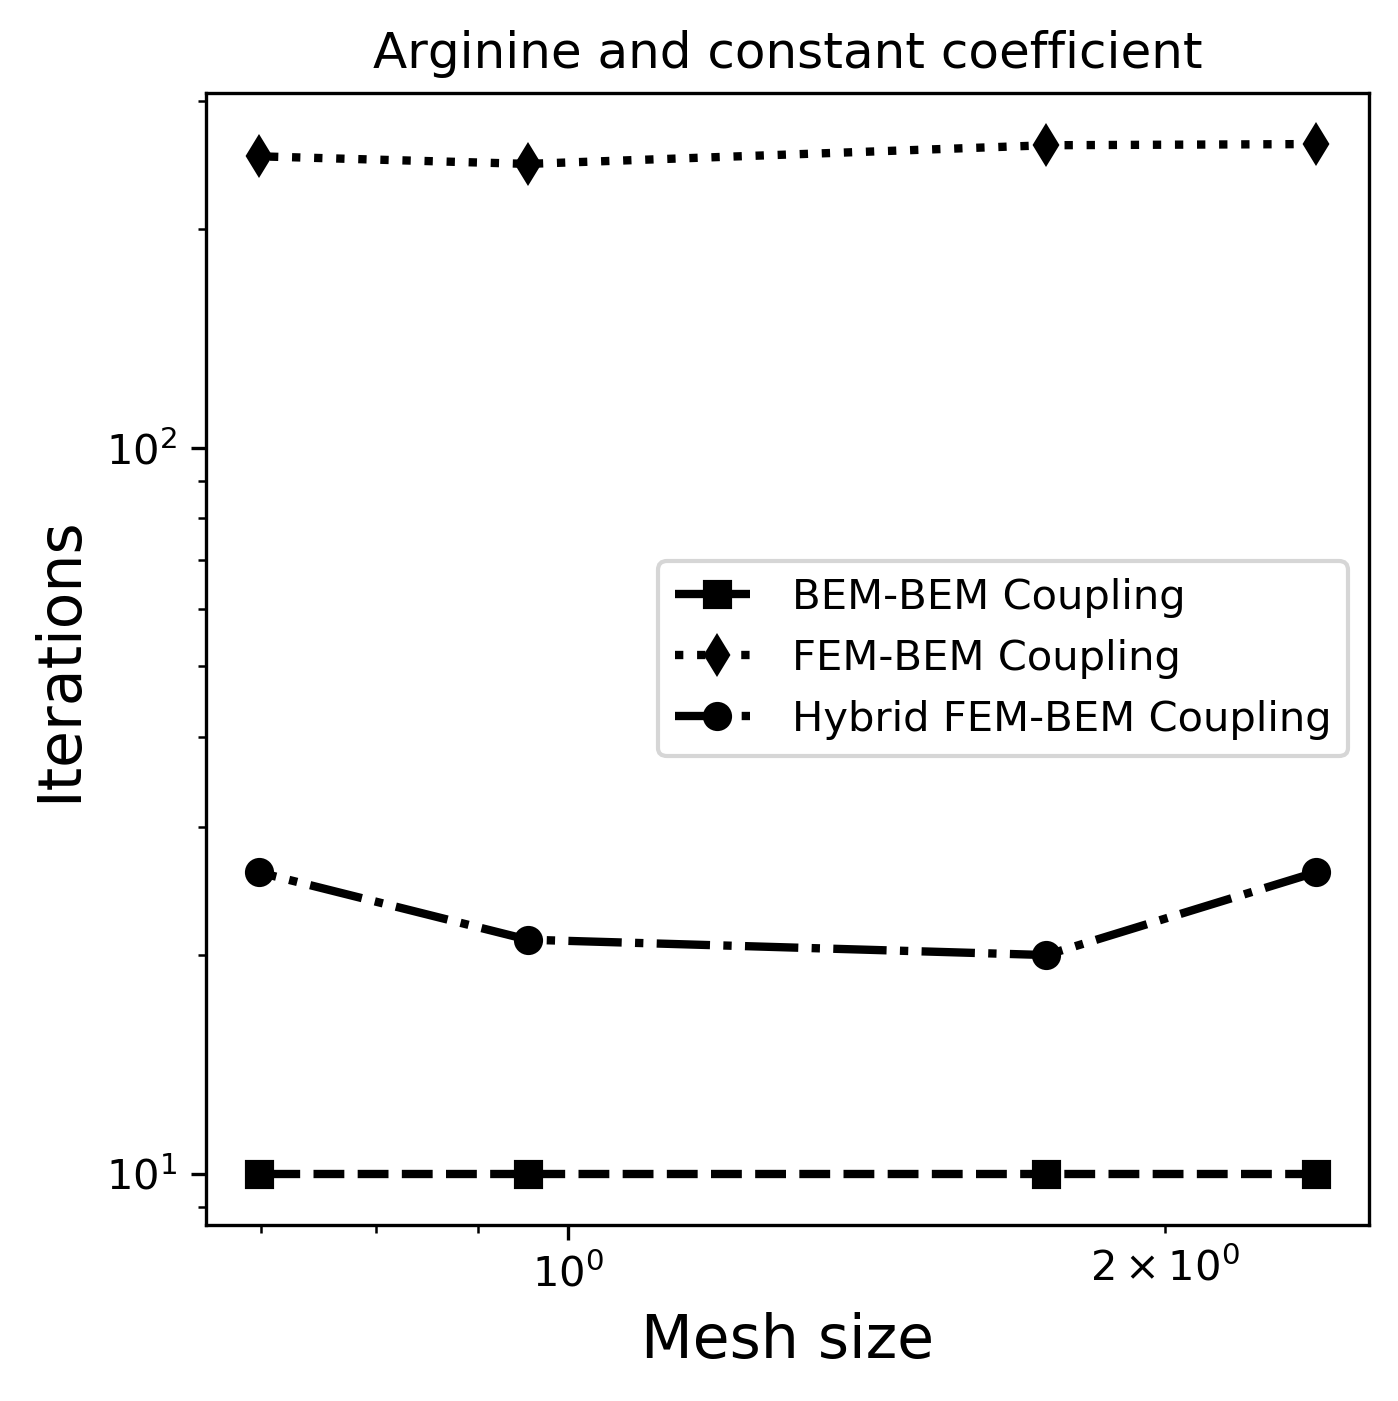
\includegraphics[width=0.6\linewidth]{Arginine_const_coeff_iter.png}
%   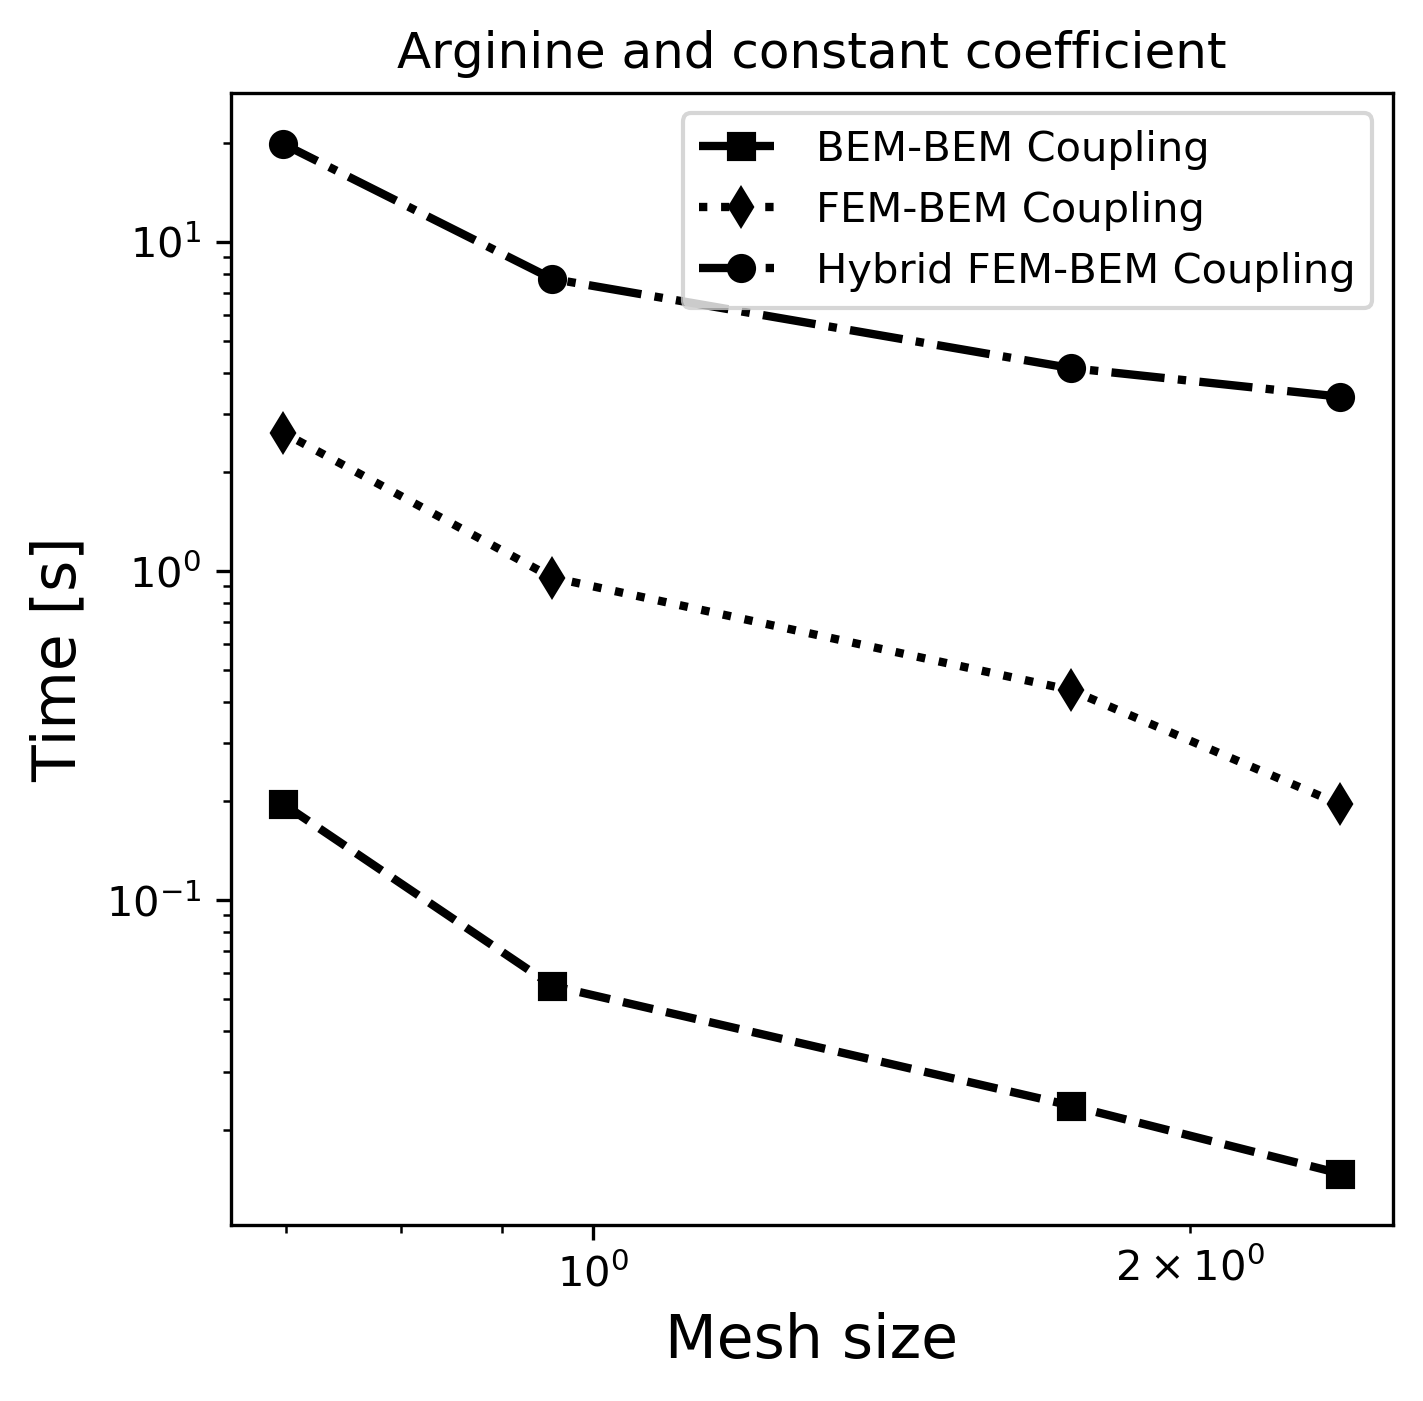
\includegraphics[width=0.45\linewidth]{Arginine_const_coeff_time.png}
\caption{Iteration count for arginine with a constant permittivity. %(1) fix title, (2) can we put them in a single plot, (3) hybrid is internal or external iterations? maybe we should present the total count?
}
\label{fig:arg_contant_iter}
\end{figure}


%\begin{itemize}
%    \item Use arginine or a small protein (1PGB?)
%    \begin{itemize}
%        \item BEM-BEM
%\begin{figure}[!htb]
%\minipage{0.45\textwidth}
%  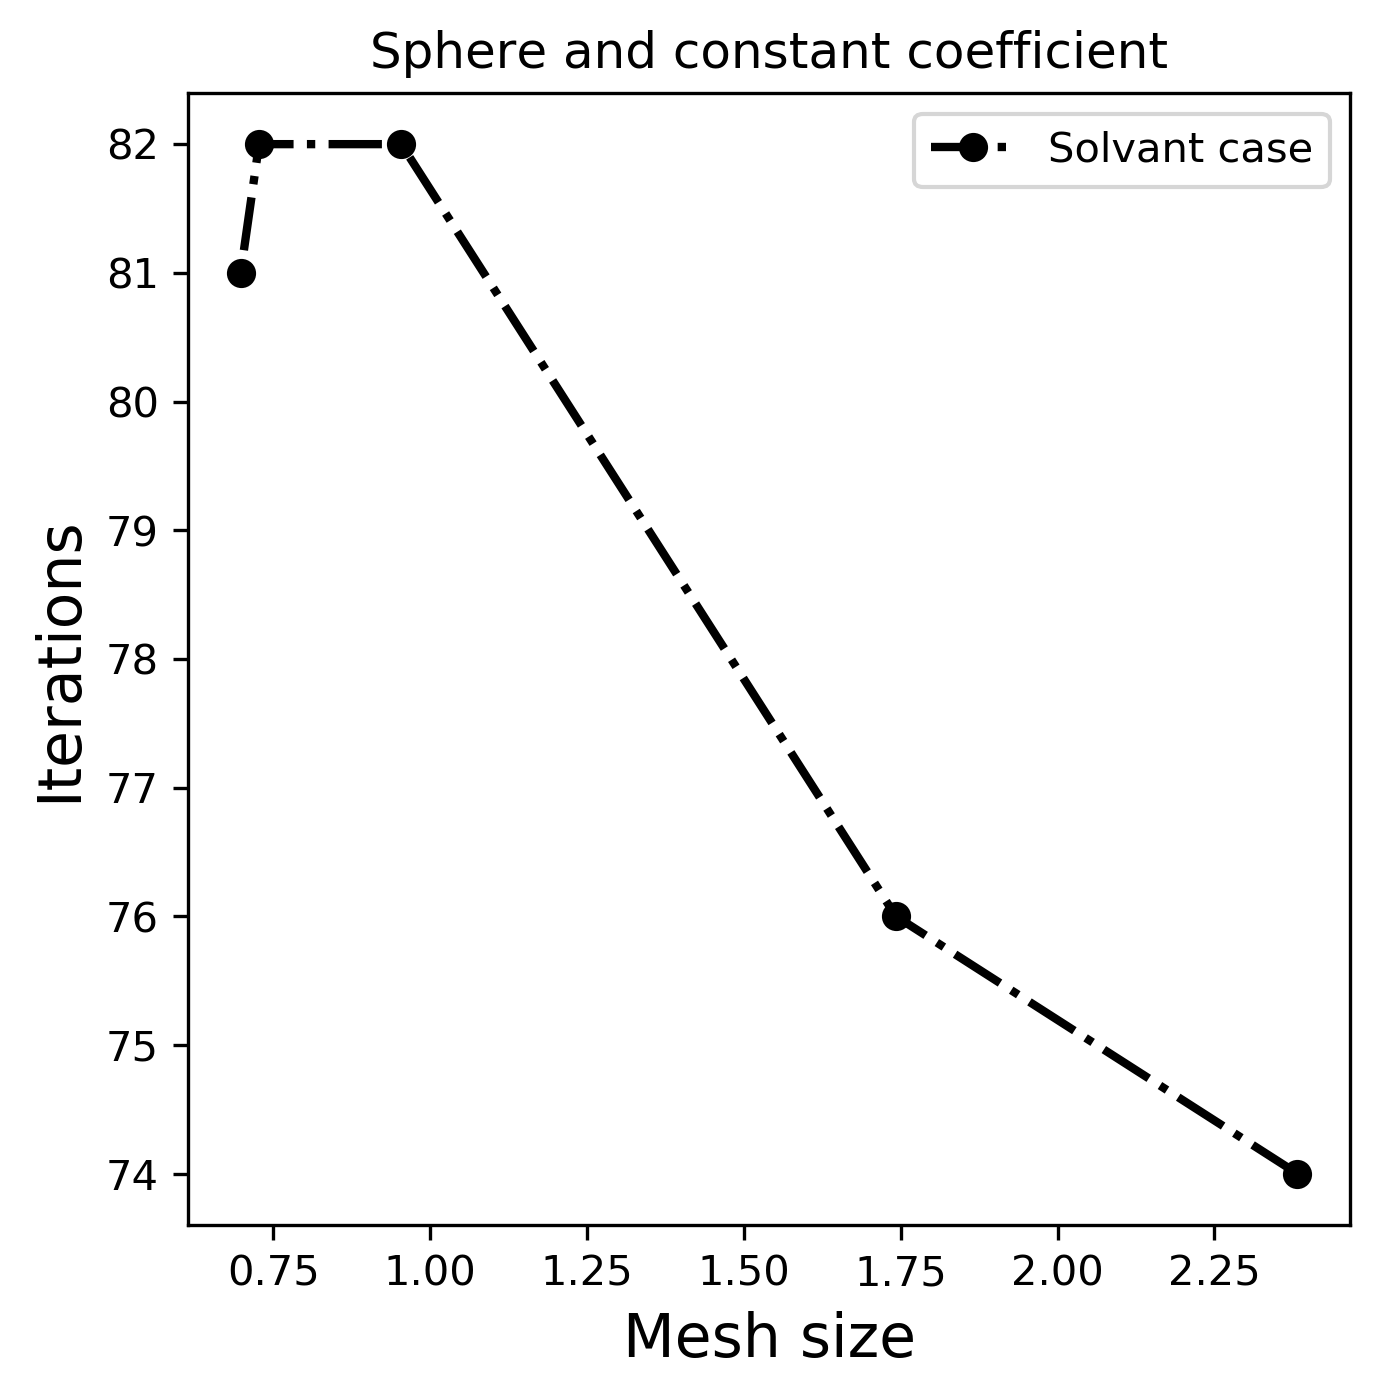
\includegraphics[width=\linewidth]{BEM_BEM_Arginine_const_coeff_iter.png}
%  \caption{Iterations}
%\endminipage\hfill
%\minipage{0.45\textwidth}%
%  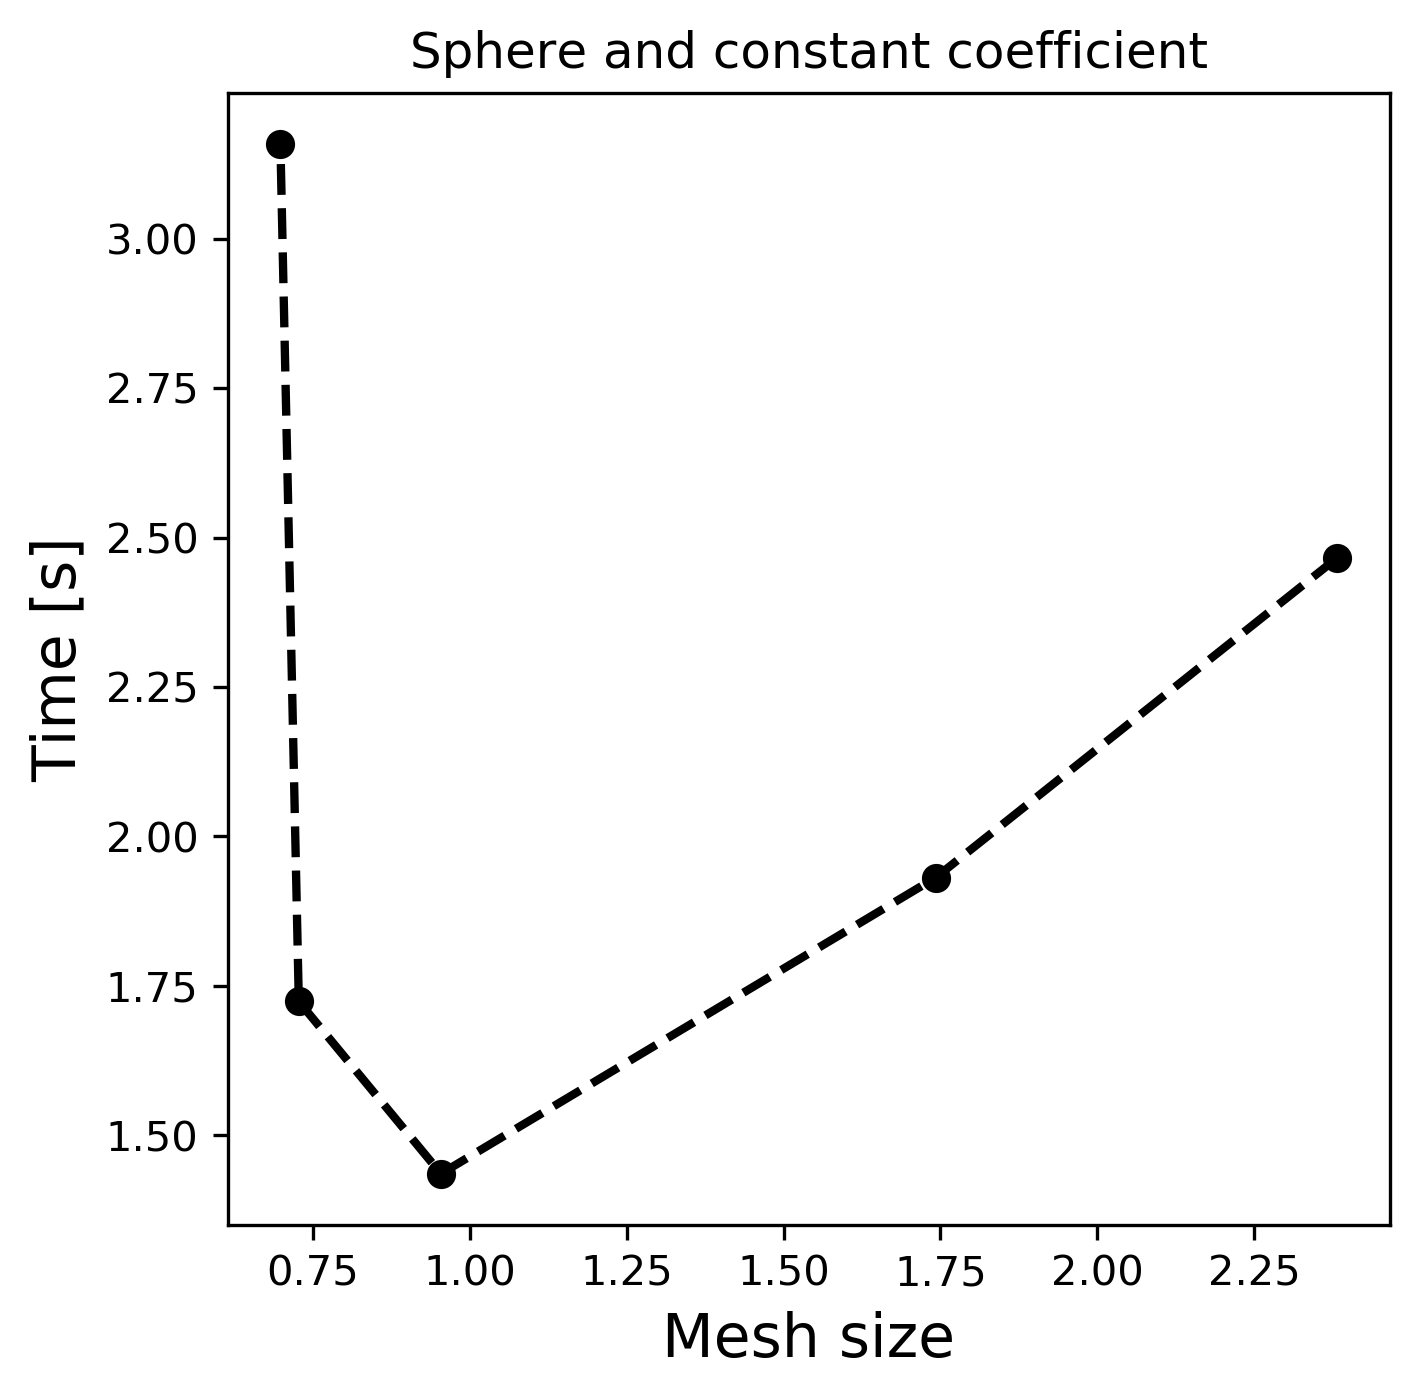
\includegraphics[width=\linewidth]{BEM_BEM_Arginine_const_coeff_time.png}
%  \caption{Computational time}
%\endminipage
%\end{figure}
%        \item Standard FEM-BEM
%\begin{figure}[!htb]
%\minipage{0.45\textwidth}
%  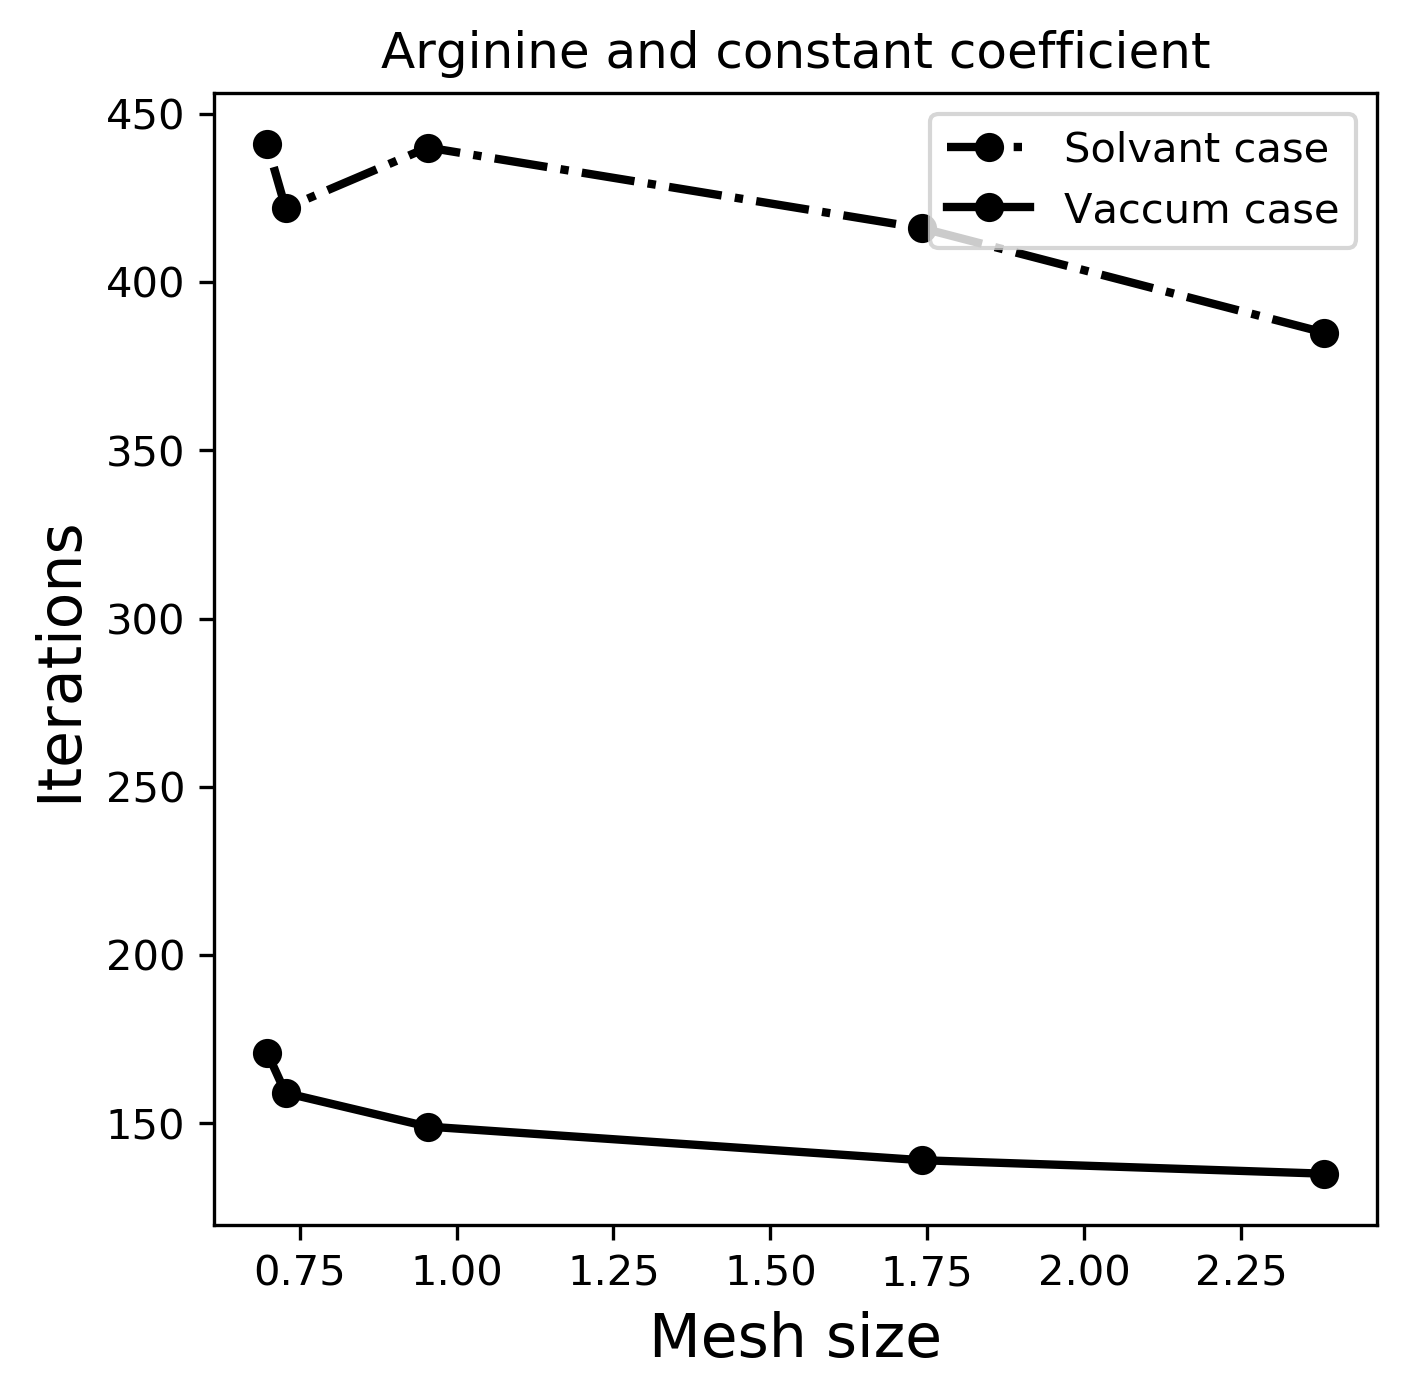
\includegraphics[width=\linewidth]{FEM_BEM_Arginine_const_coeff_iter.png}
%  \caption{Iterations}
%\endminipage\hfill
%\minipage{0.45\textwidth}%
%  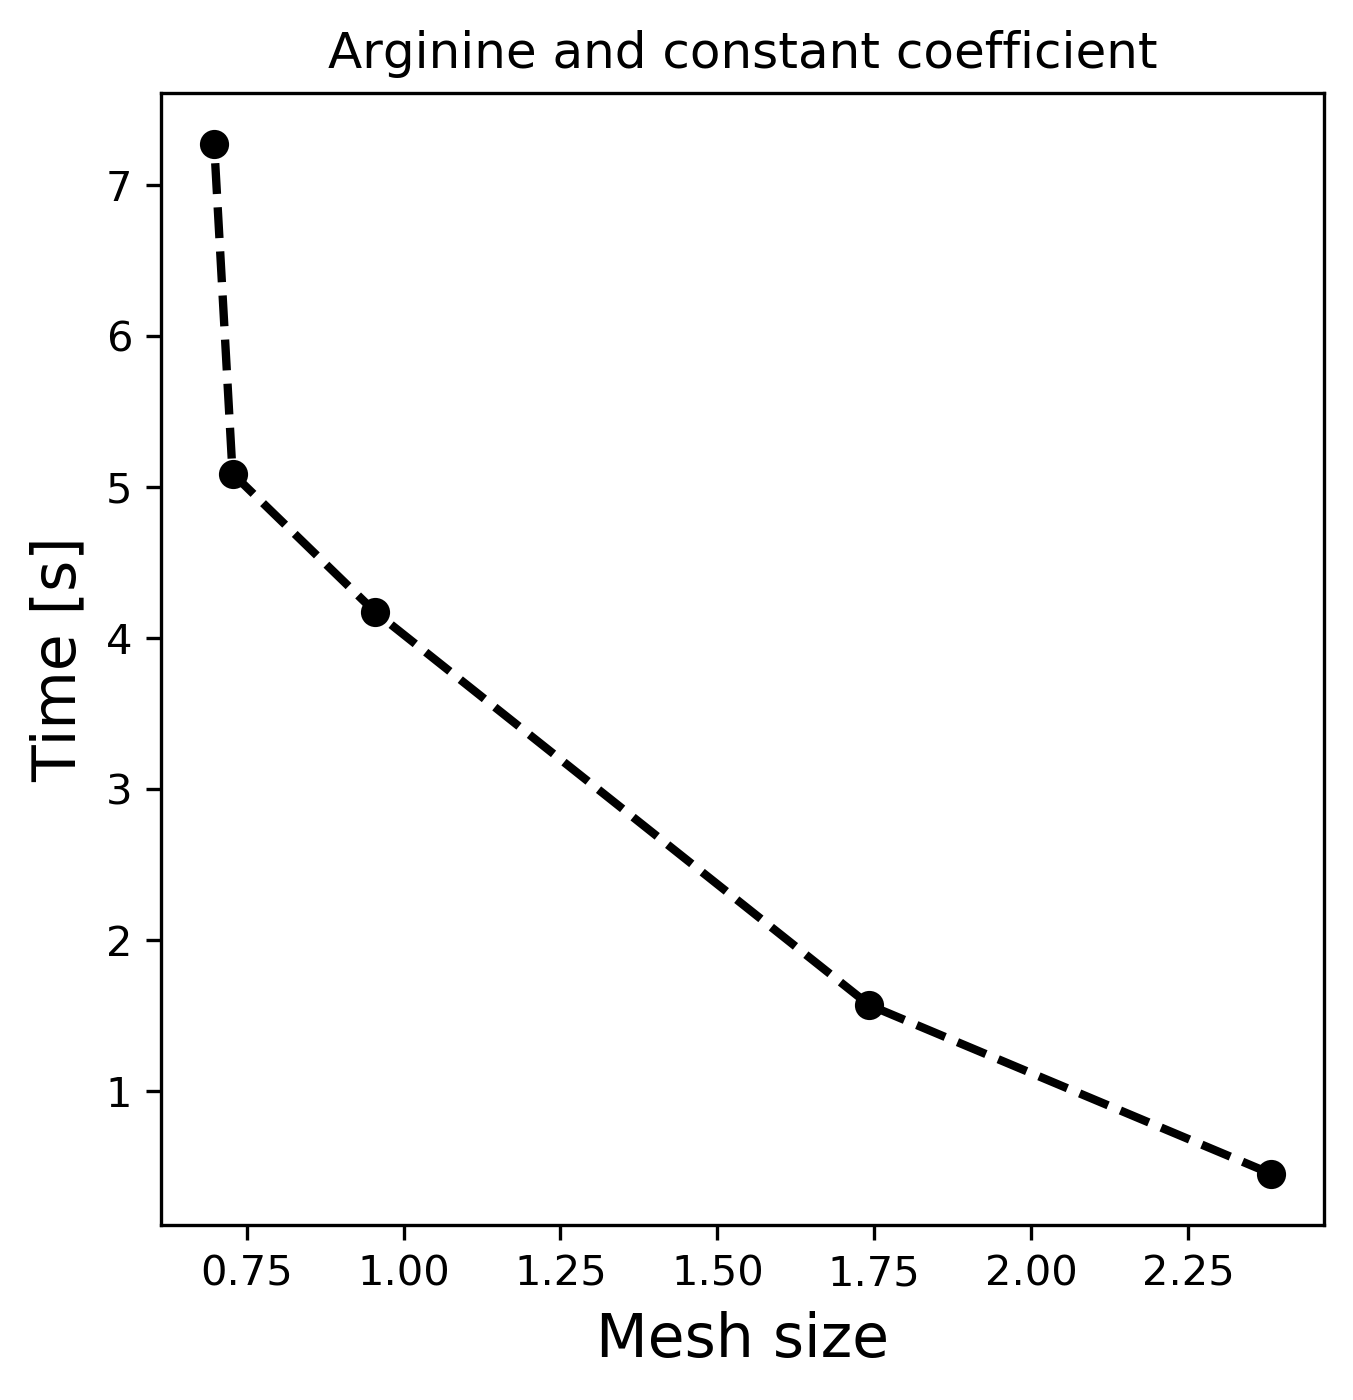
\includegraphics[width=\linewidth]{FEM_BEM_Arginine_const_coeff_time.png}
%  \caption{Computational time}
%\endminipage
%\end{figure}
%        \item Hybrid FEM-BEM
%\begin{figure}[!htb]
%\minipage{0.45\textwidth}
%  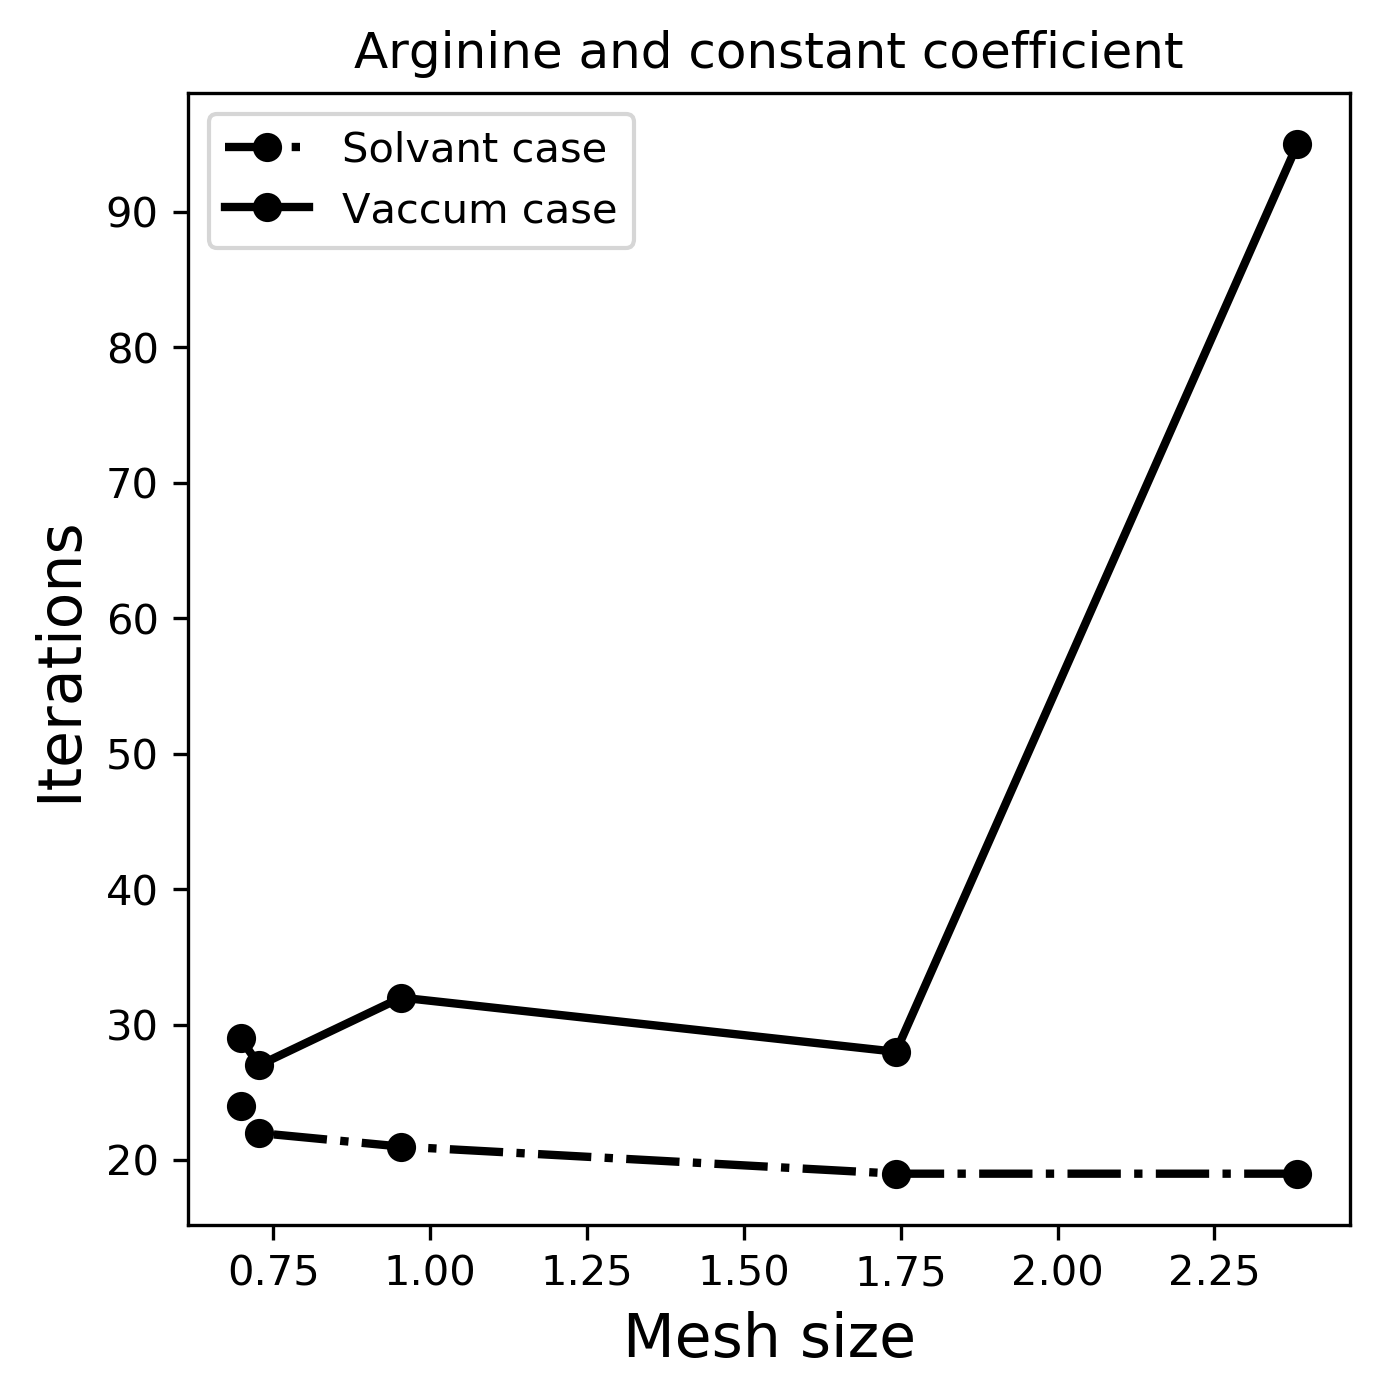
\includegraphics[width=\linewidth]{Hybrid_FEM_BEM_Arginine_const_coeff_iter.png}
%  \caption{Iterations}
%\endminipage\hfill
%\minipage{0.45\textwidth}%
%  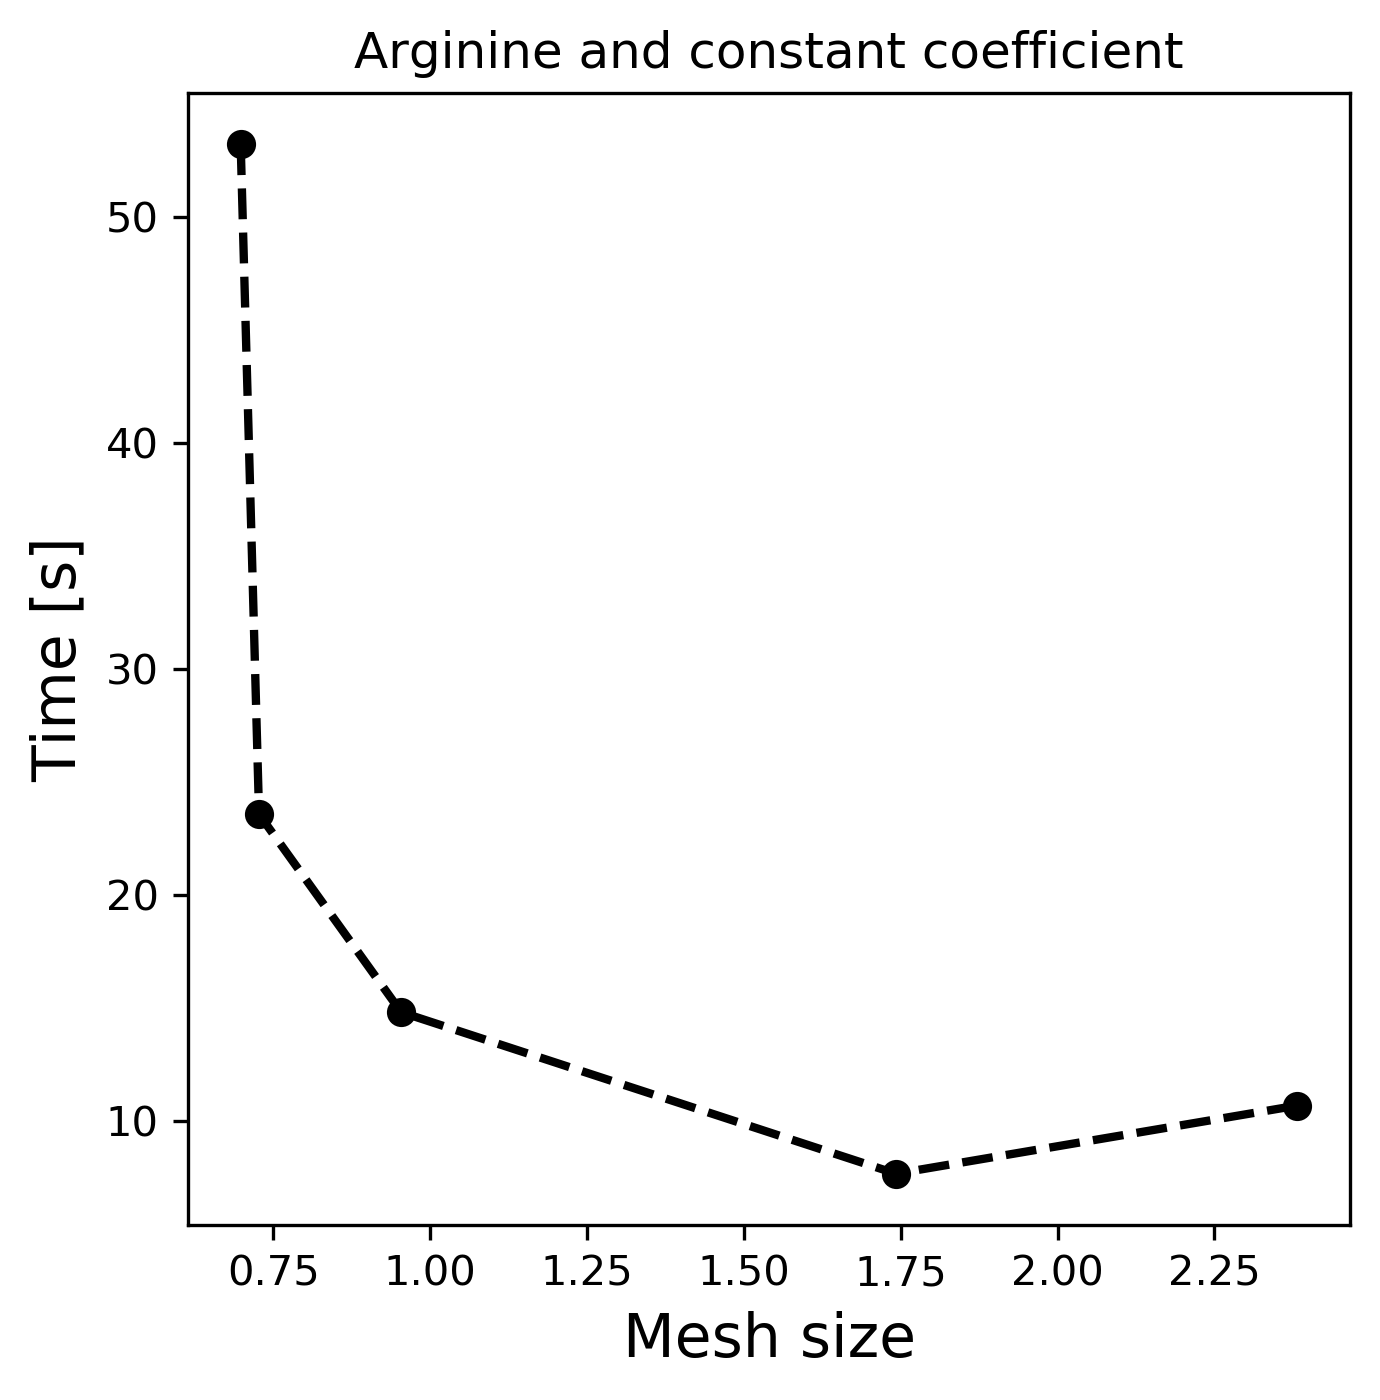
\includegraphics[width=\linewidth]{Hybrid_FEM_BEM_Arginine_const_coeff_time.png}
%  \caption{Computational time}
%\endminipage
%\end{figure}
%    \end{itemize}
%    \item Compare computer time and iterations for FEM-BEM with standard and hybrid approaches, without preconditioner. Choose hybrid.
%    \item Show performance of hybrid method with preconditioner.
%\end{itemize}

\section*{\sffamily \Large Results with variable permittivity}

In contrast to a purely BEM approach, FEM-BEM coupling gives flexibility to consider space-varying field parameters. 
A popular description of the molecule is to consider a permittivity that varies like a Gaussian around each atom [earlier papers], which has shown enhanced accuracy in some applications, like binding energy calculations (check) [Alexov].
In this setting, we define a density function $\rho$ depending on position $r$ as
%
\begin{equation}
\rho(r) := \prod_i \left(1 - \exp{\left(\frac{\|r-\mathbf{x}_i\|}{\sigma^2 R_i^2}\right)}\right)
\end{equation}
%
where the product is over the atoms of the solute, $R_i$ is the vdW
radius of atom i and we used $\sigma$=1. Then, we can compute the permittivity as
%
\begin{equation}
\epsilon := \left(1-\rho \right) \epsilon_1 + \rho\epsilon_2
\end{equation}
%

We used Equation \eqref{eq:epsilon_gauss} to generate dielectric maps, which we ran on APBS for comparison. 
As $\epsilon_2$ is variable, Equation \eqref{eq:phi_coulomb} does not have an analytical solution, and the electrostatic potential in vacuum state has to be computed numerically.
For vacuum calculations, we considered the same distribution of $\epsilon$ inside the molecule as in the solvated case, however, the solvent permittivity was set to $\epsilon$=2. 
Other implementations of Gaussian permittivities also modify the solute permittivity in vacuum calculations, according to a set cutoff [Alexov]. 
We did not consider a cutoff in our calculations, but this does not affect our validation exercise. 

\subsection*{\sffamily \large Convergence and performance for arginine}

Table \ref{table:arg_variable} shows a comparison of solvation energy computed with APBS and our FEM-BEM coupling approaches. We can see that they are both converging to equivalent values of solvation energy, where the finest meshes agree up to the third significant figure.

Figure \ref{fig:arg_variable} contains performance results of this test case, where we distinguish the iteration count from the calculation in dissolved and vacuum states. 
Similar to the case with constant permittivity, although the hybrid approach requires less iterations (are we counting them appropriately? meaning there are external and internal iterations), the total time to solution is less for the standard approach. This means that each iteration of hybrid FEM-BEM is slower than the standard counterpart.


\begin{table}
\centering
\begin{tabular}{c|c|c}
&Mesh size & $\Delta G_{solv}$\\
&\AA       &  kcal/mol \\
\hline
\multirow{3}{*}{APBS}& 0.39$\times$0.39$\times$0.39 & -32.4042\\ 
&0.26$\times$0.26$\times$0.26 & -32.3375\\ 
&0.17$\times$0.17$\times$0.17 & -32.3413\\ 
\hline
&Mesh dens. & \\
&vert/\AA$^2$ & \\
\hline
%\multirow{5}{*}{Standard FEM-BEM}& 2 & -36.239\\
    & 2 & -36.239\\
Standard    & 4  & -33.129 \\
FEM-BEM    & 8  & -32.674 \\
    & 12 & -32.648 \\
    & 16 & -32.293 \\
\hline
%\multirow{5}{*}{Standard FEM-BEM}& 2 & -29.554\\
    & 2 & -35.333\\
Hybrid    & 4  & -33.079 \\
FEM-BEM    & 8  & -32.660 \\
    & 12 & -32.587 \\
    & 16 & -32.359 \\
\hline
\end{tabular}
\caption{Solvation energy of arginine with a Gaussian-like permittivity, computed using the standard and hybrid FEM-BEM approaches, and APBS.}
\label{table:arg_variable}
\end{table}

\begin{figure}
\centering
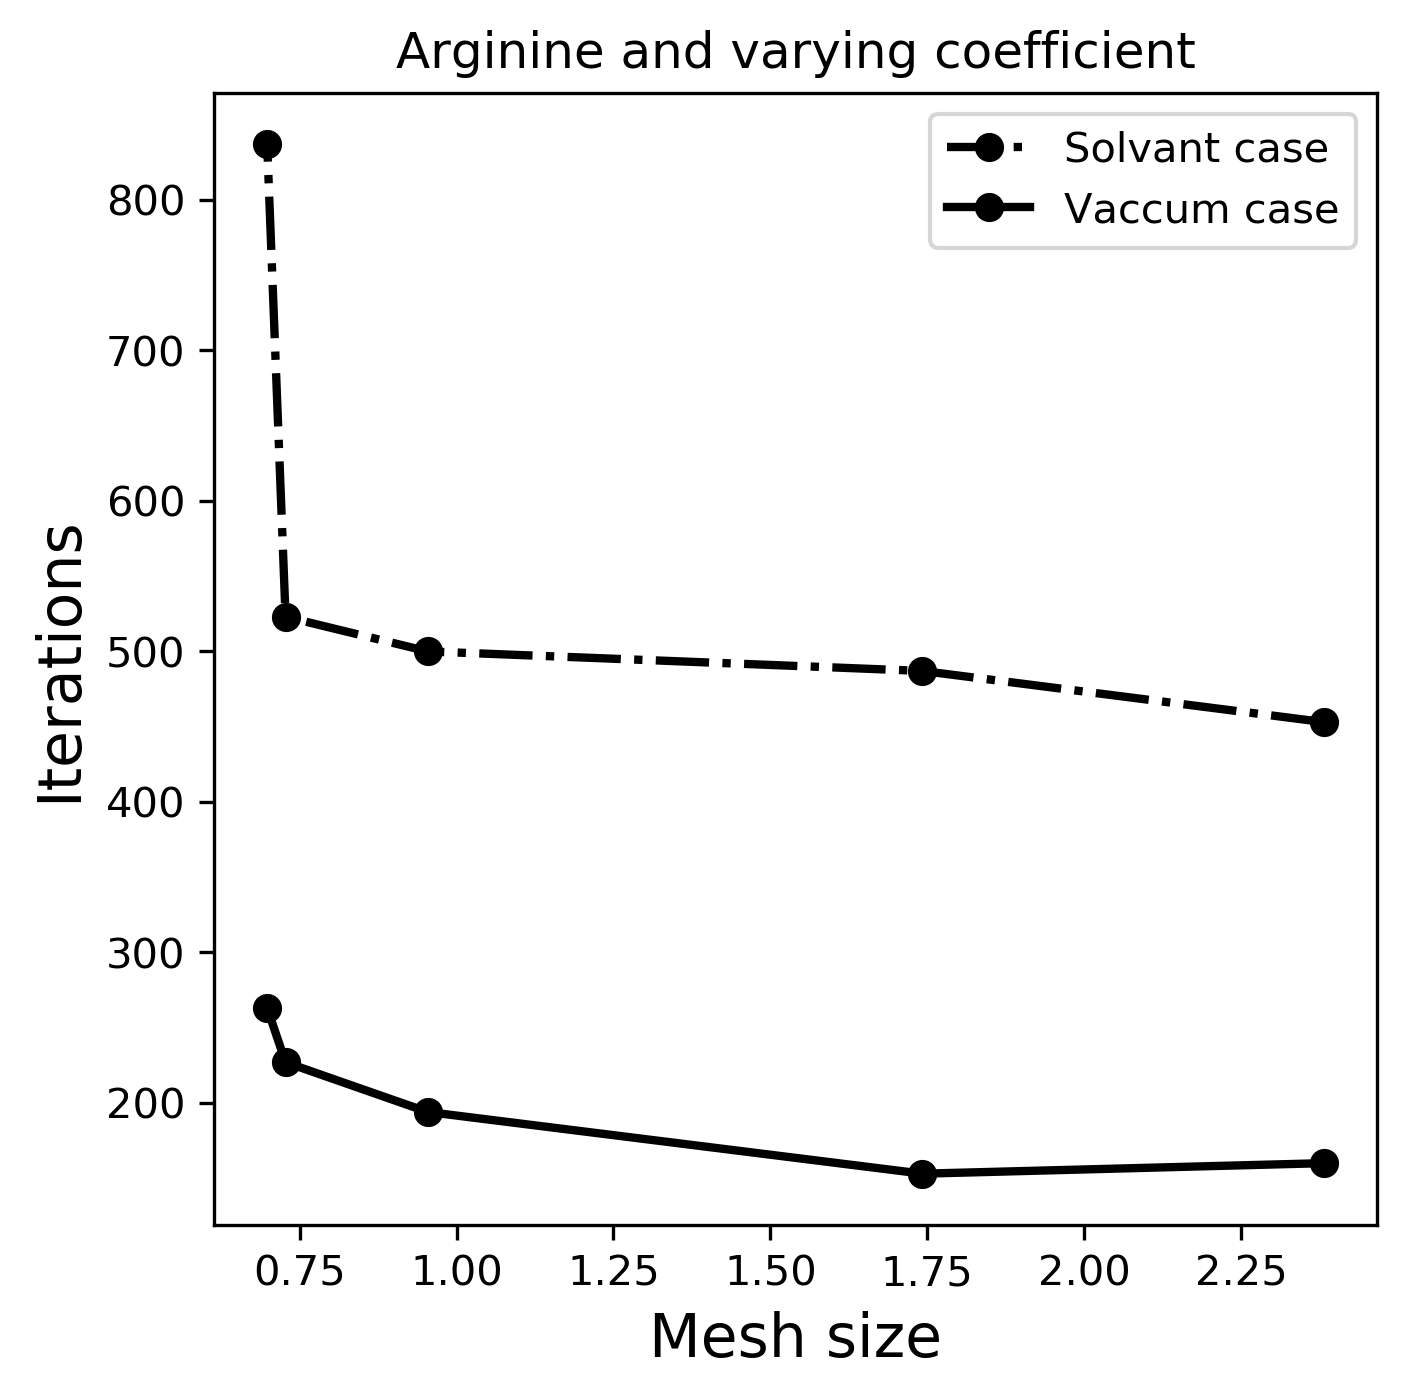
\includegraphics[width=0.45\linewidth]{FEM_BEM_Arginine_varying_coeff_iter.png}
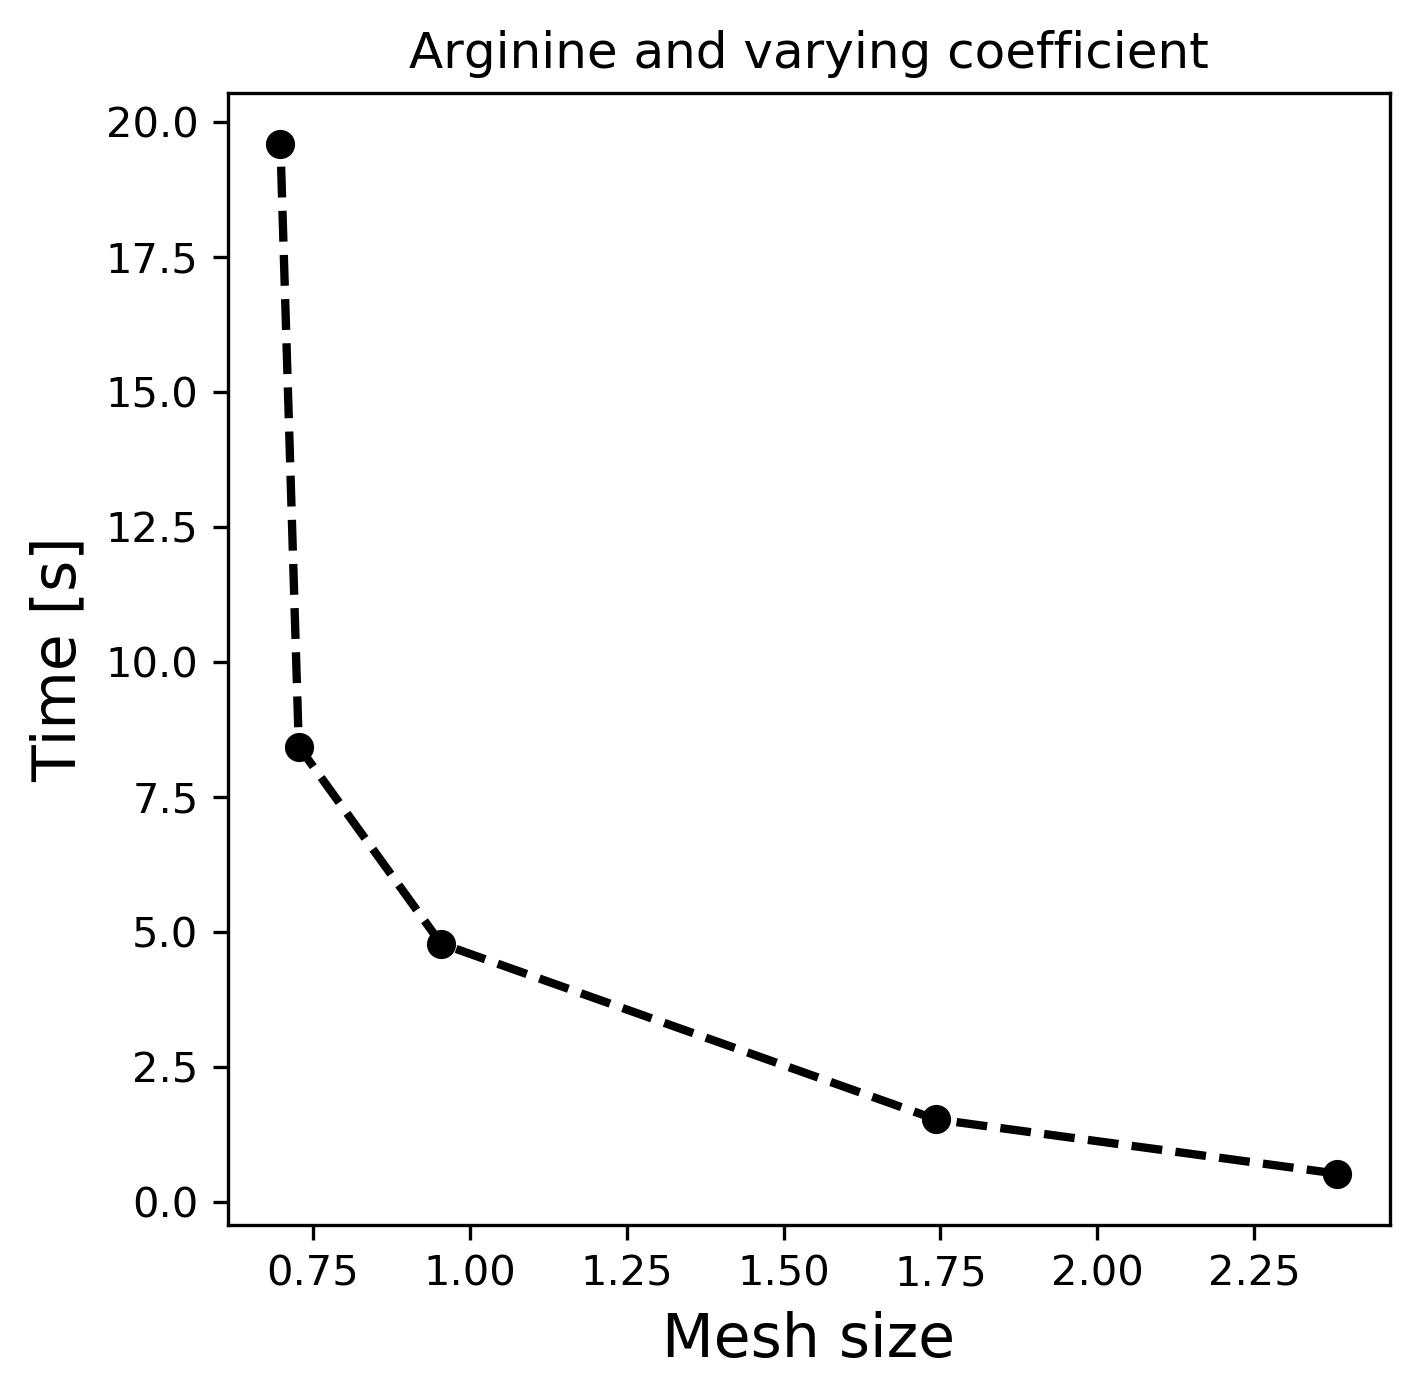
\includegraphics[width=0.45\linewidth]{FEM_BEM_Arginine_varying_coeff_time.png}
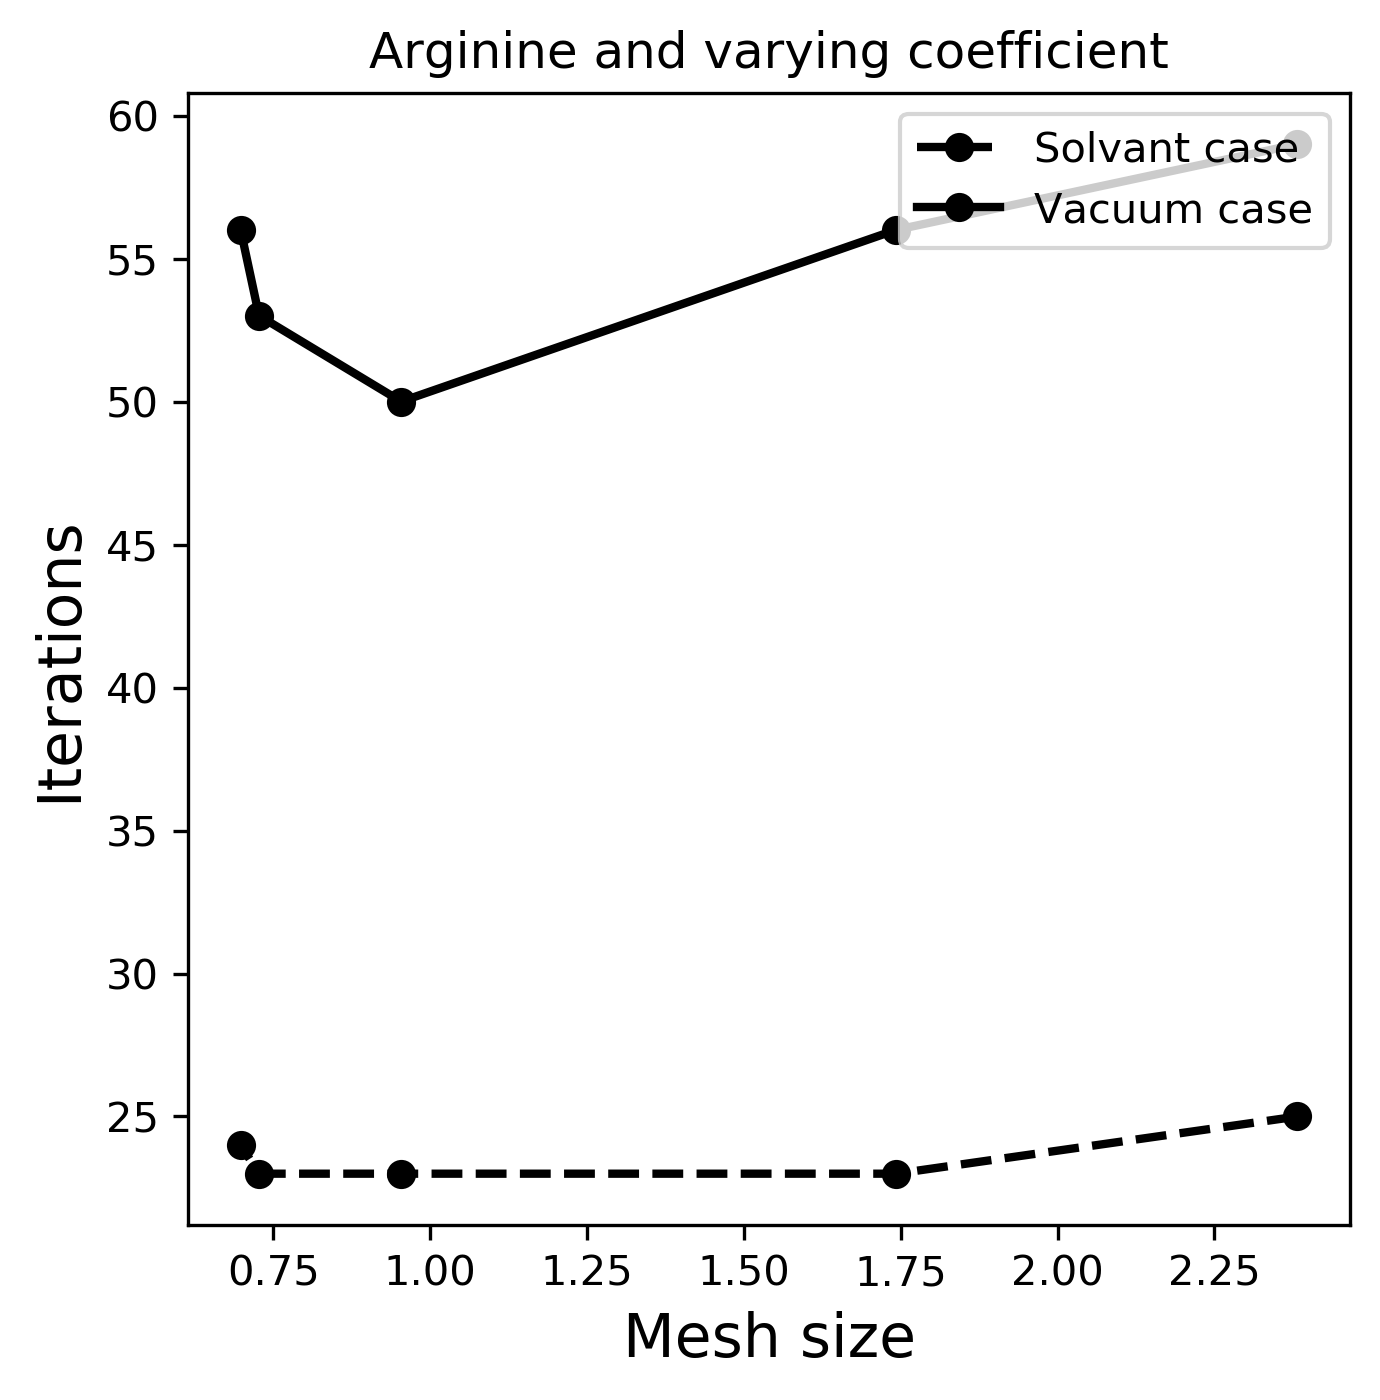
\includegraphics[width=0.45\linewidth]{Hybrid_FEM_BEM_Arginine_varying_coeff_iter.png}
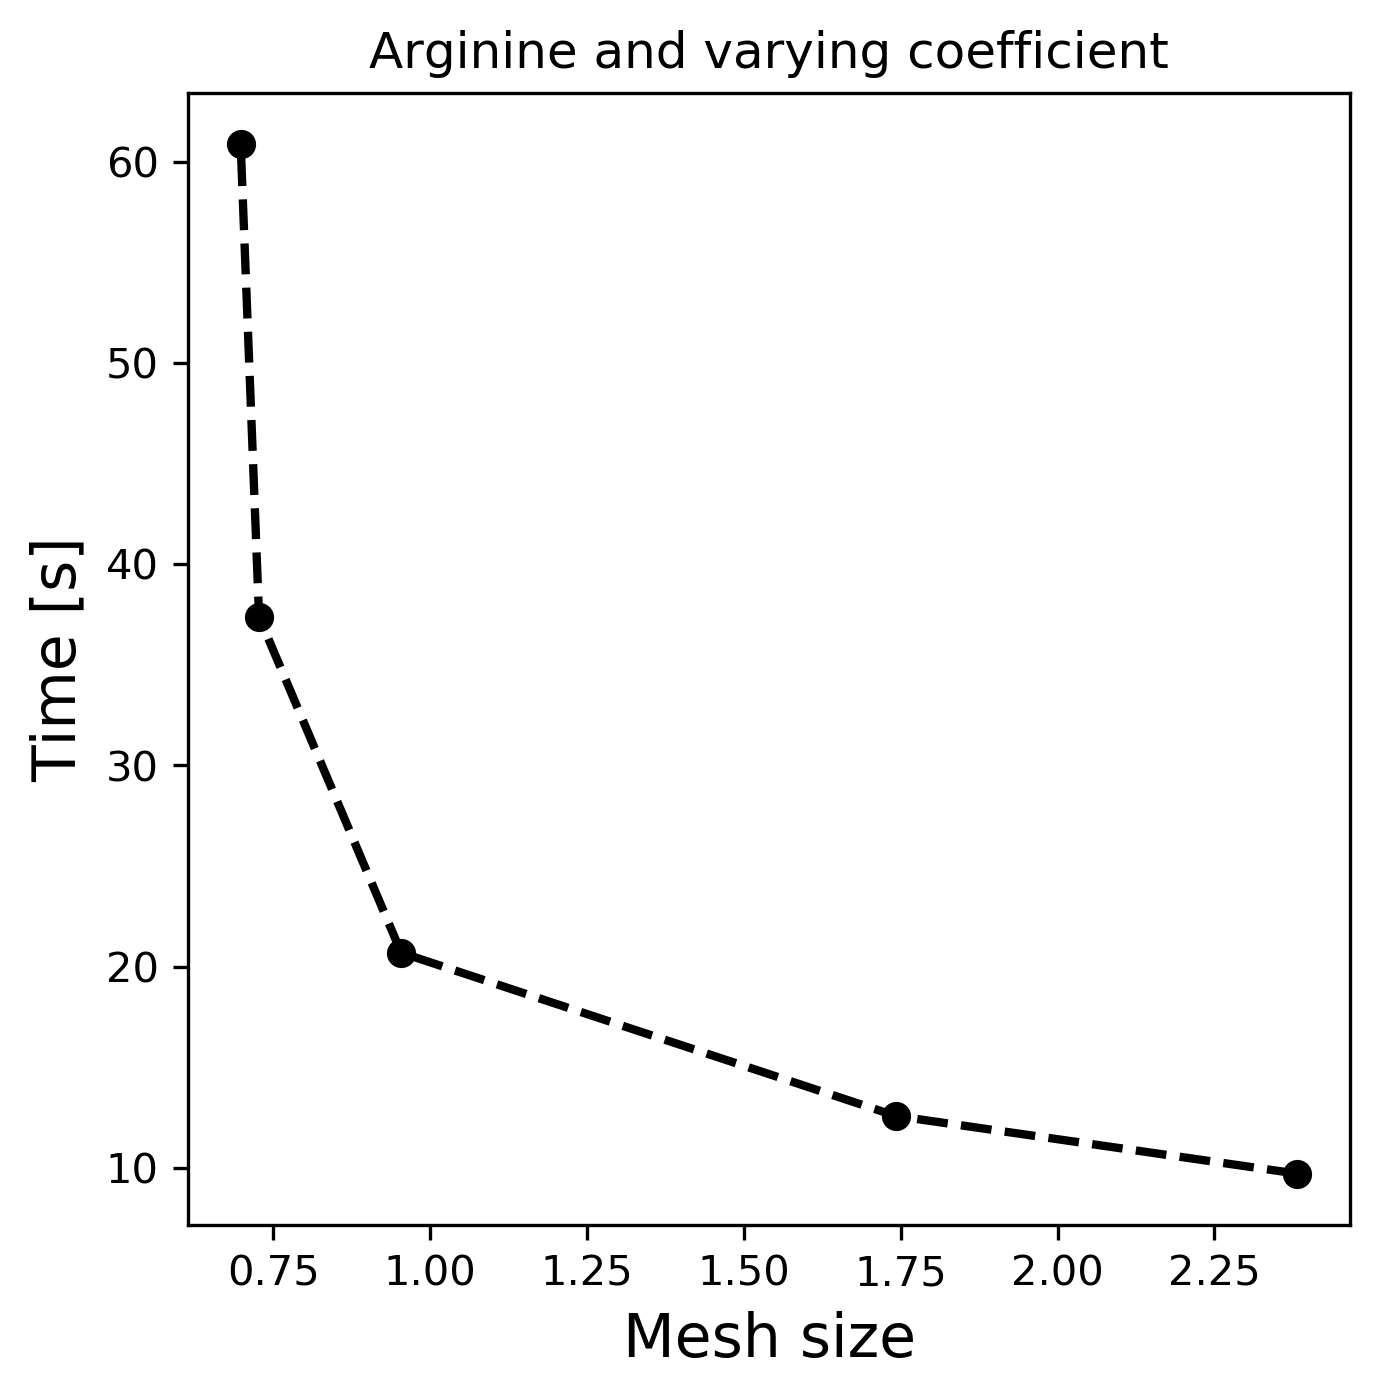
\includegraphics[width=0.45\linewidth]{Hybrid_FEM_BEM_Arginine_varying_coeff_time.png}
\caption{Time-to-solution and iteration count to compute the solvation energy of arginine with a variable permittivity, using standard and hybrid FEM-BEM coupling. Can we make this only two plots?}
\label{fig:arg_variable}
\end{figure}

%
%    \begin{itemize}
%        \item Standard FEM-BEM
%\begin{figure}[!htb]
%\minipage{0.45\textwidth}
%  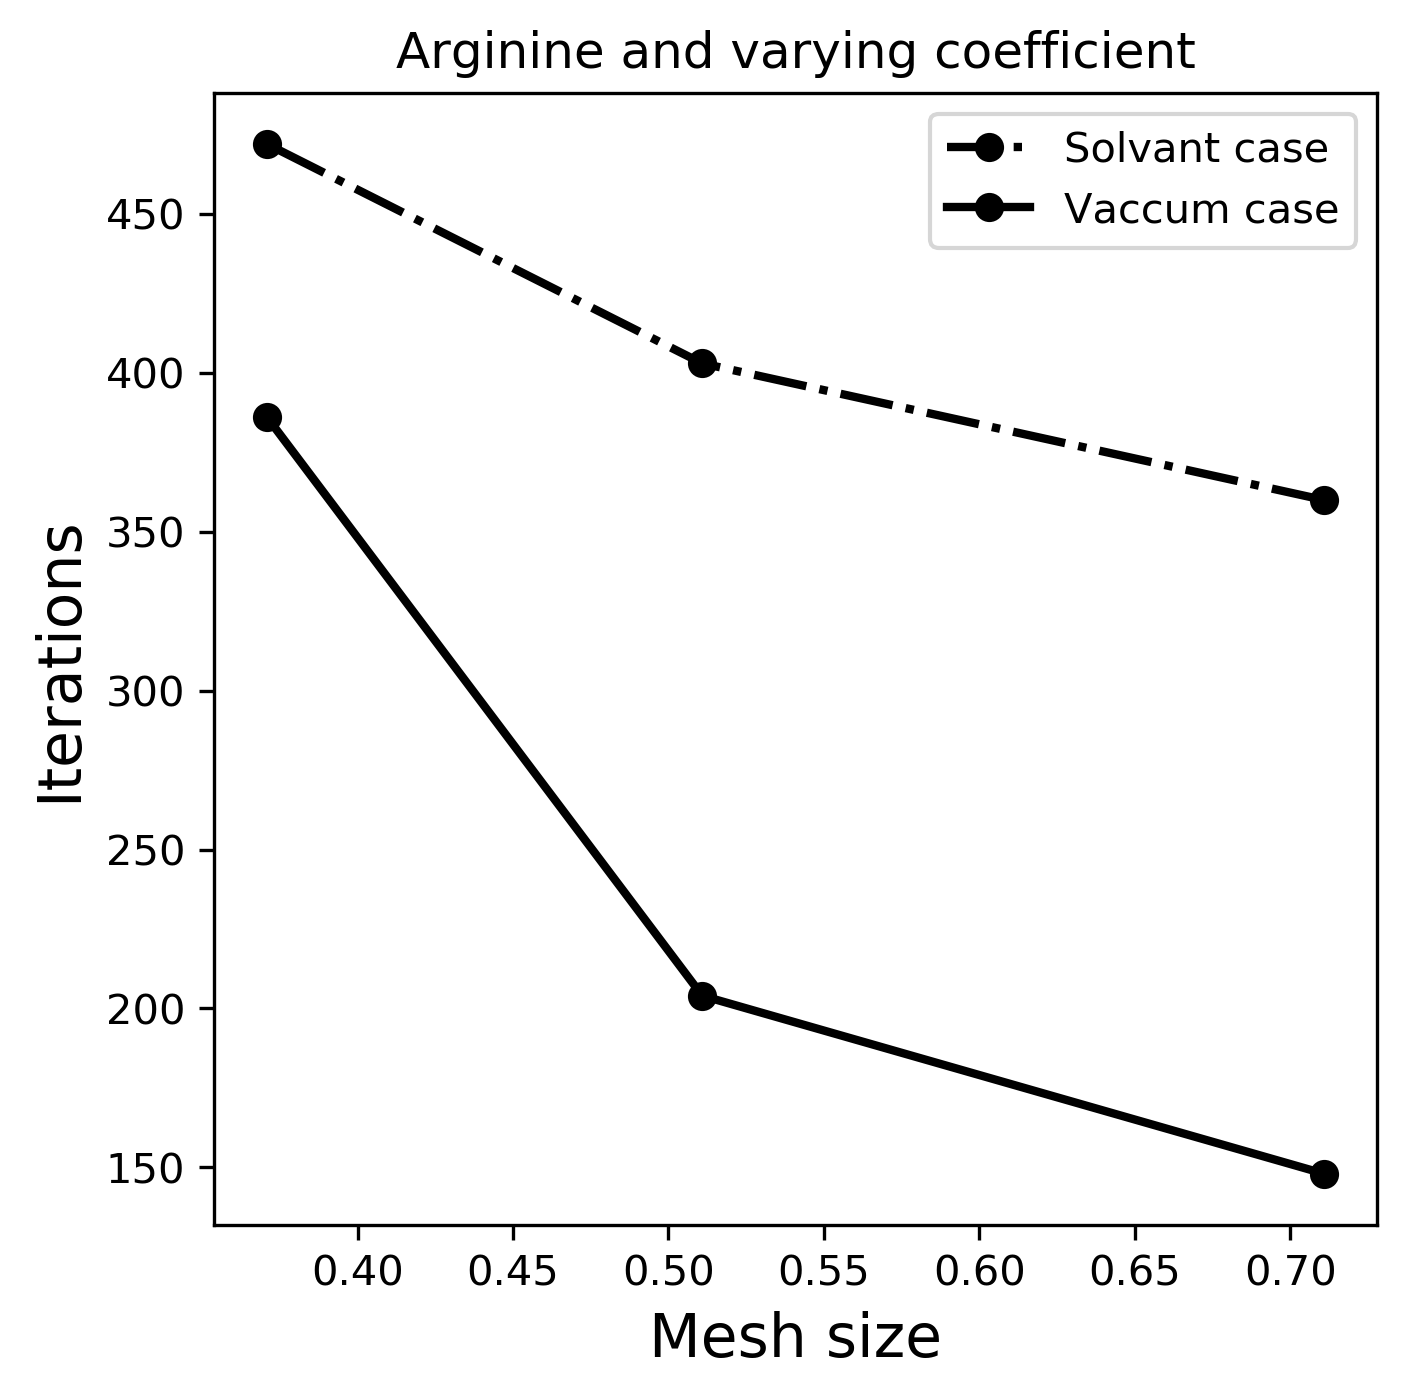
\includegraphics[width=\linewidth]{FEM_BEM_Sphere_varying_coeff_iter.png}
%  \caption{Iterations}
%\endminipage\hfill
%\minipage{0.45\textwidth}%
%  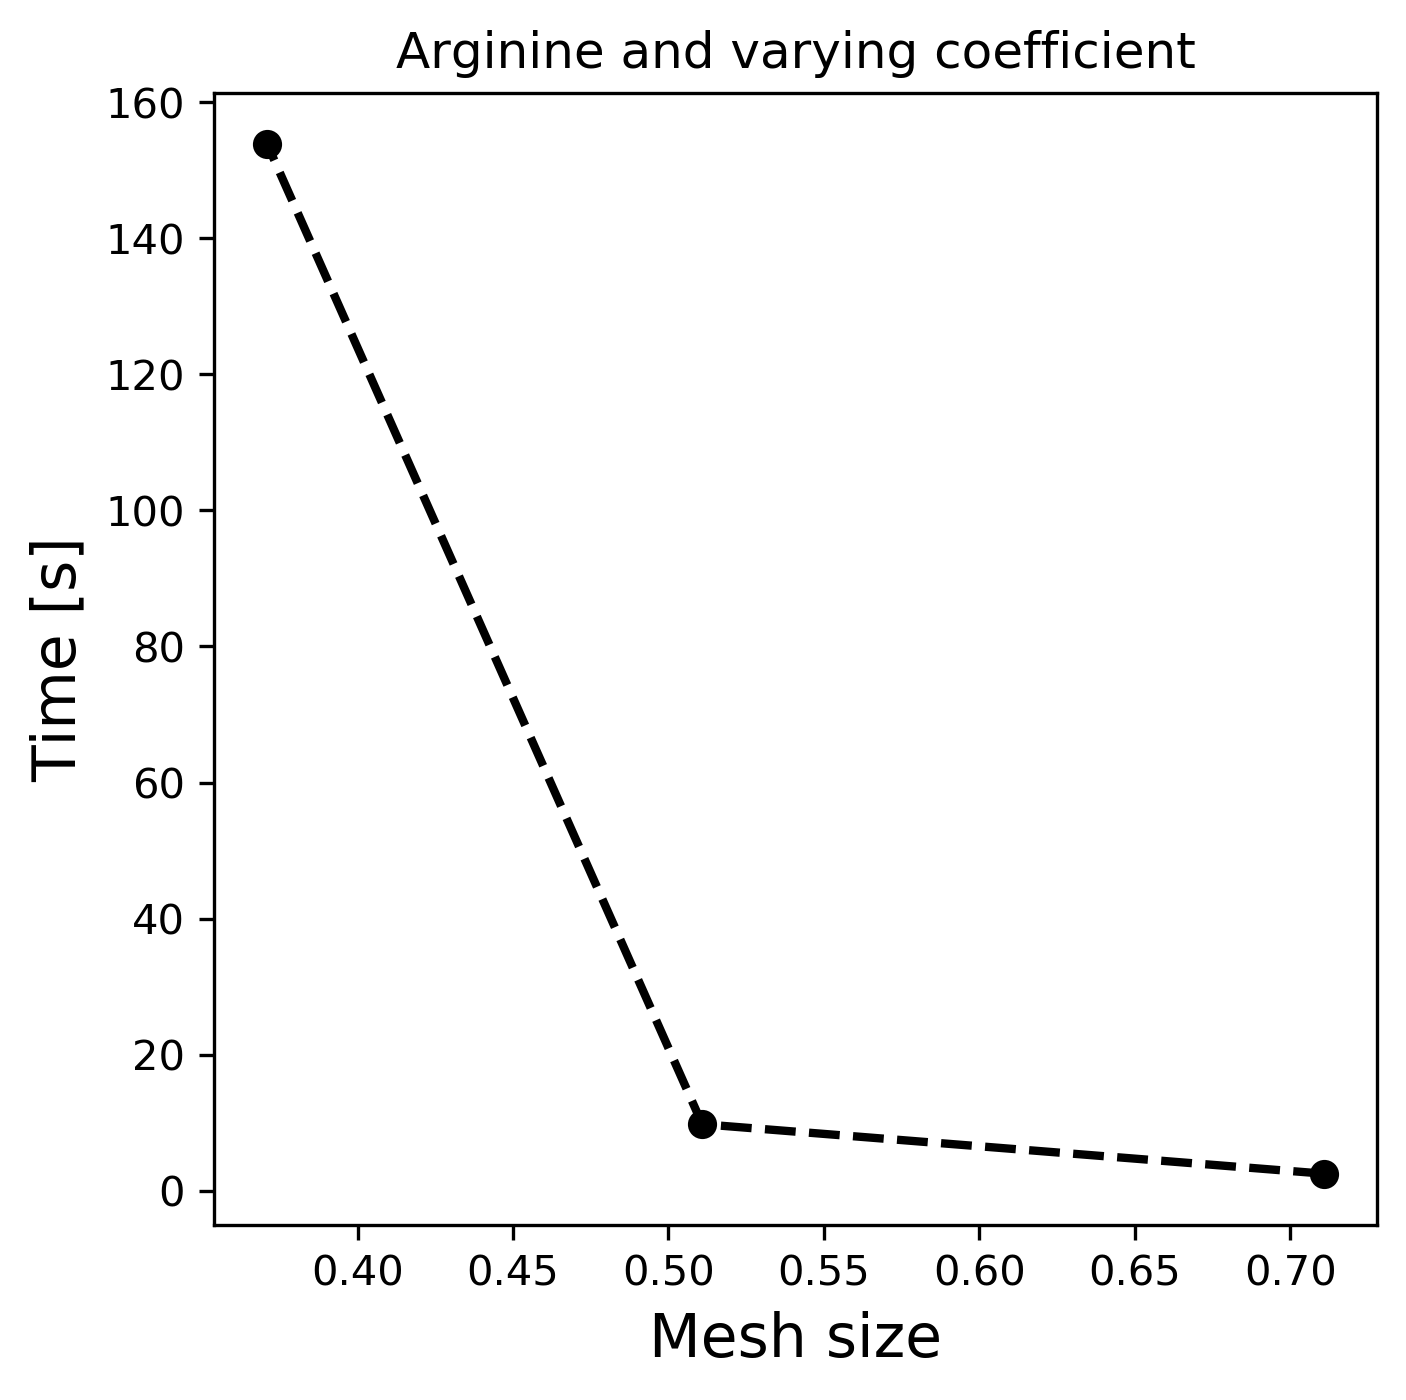
\includegraphics[width=\linewidth]{FEM_BEM_Sphere_varying_coeff_time.png}
%  \caption{Computational time}
%\endminipage
%\end{figure}
%        \item Hybrid FEM-BEM
%\begin{figure}[!htb]
%\minipage{0.45\textwidth}
%  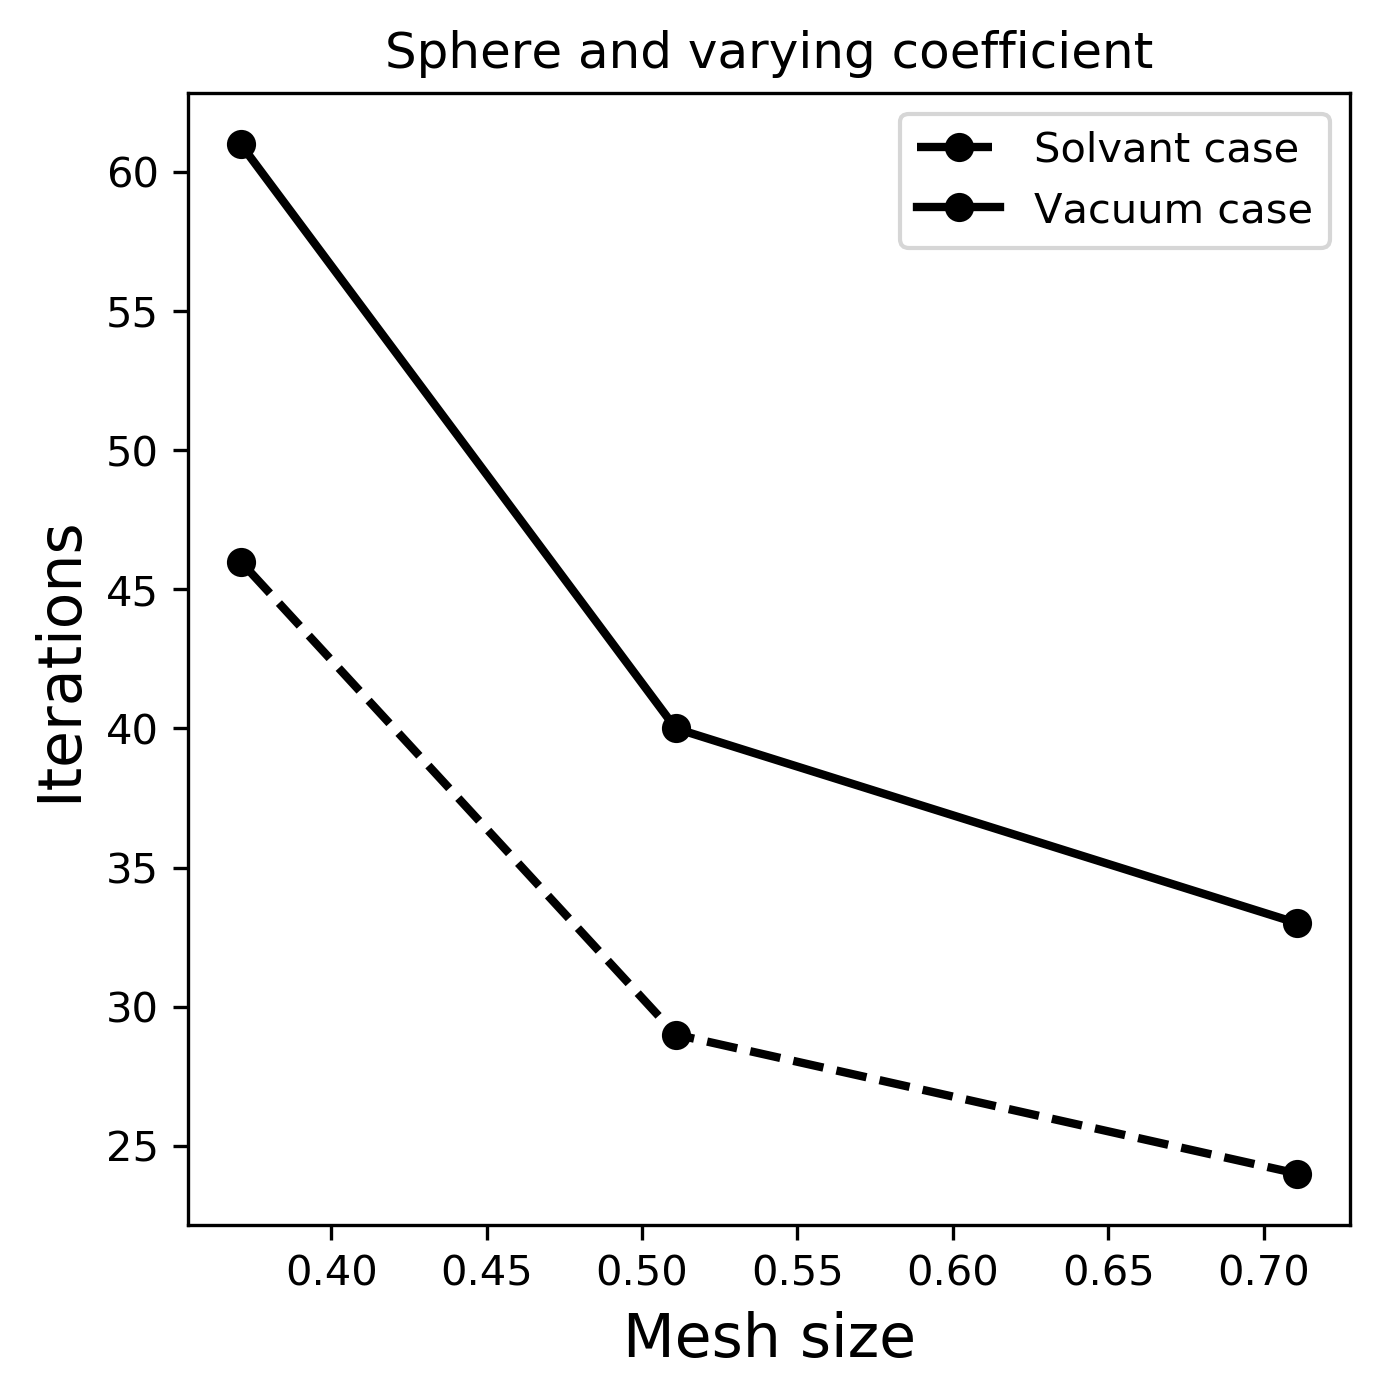
\includegraphics[width=\linewidth]{Hybrid_FEM_BEM_Sphere_varying_coeff_iter.png}
%  \caption{Iterations}
%\endminipage\hfill
%\minipage{0.45\textwidth}%
%  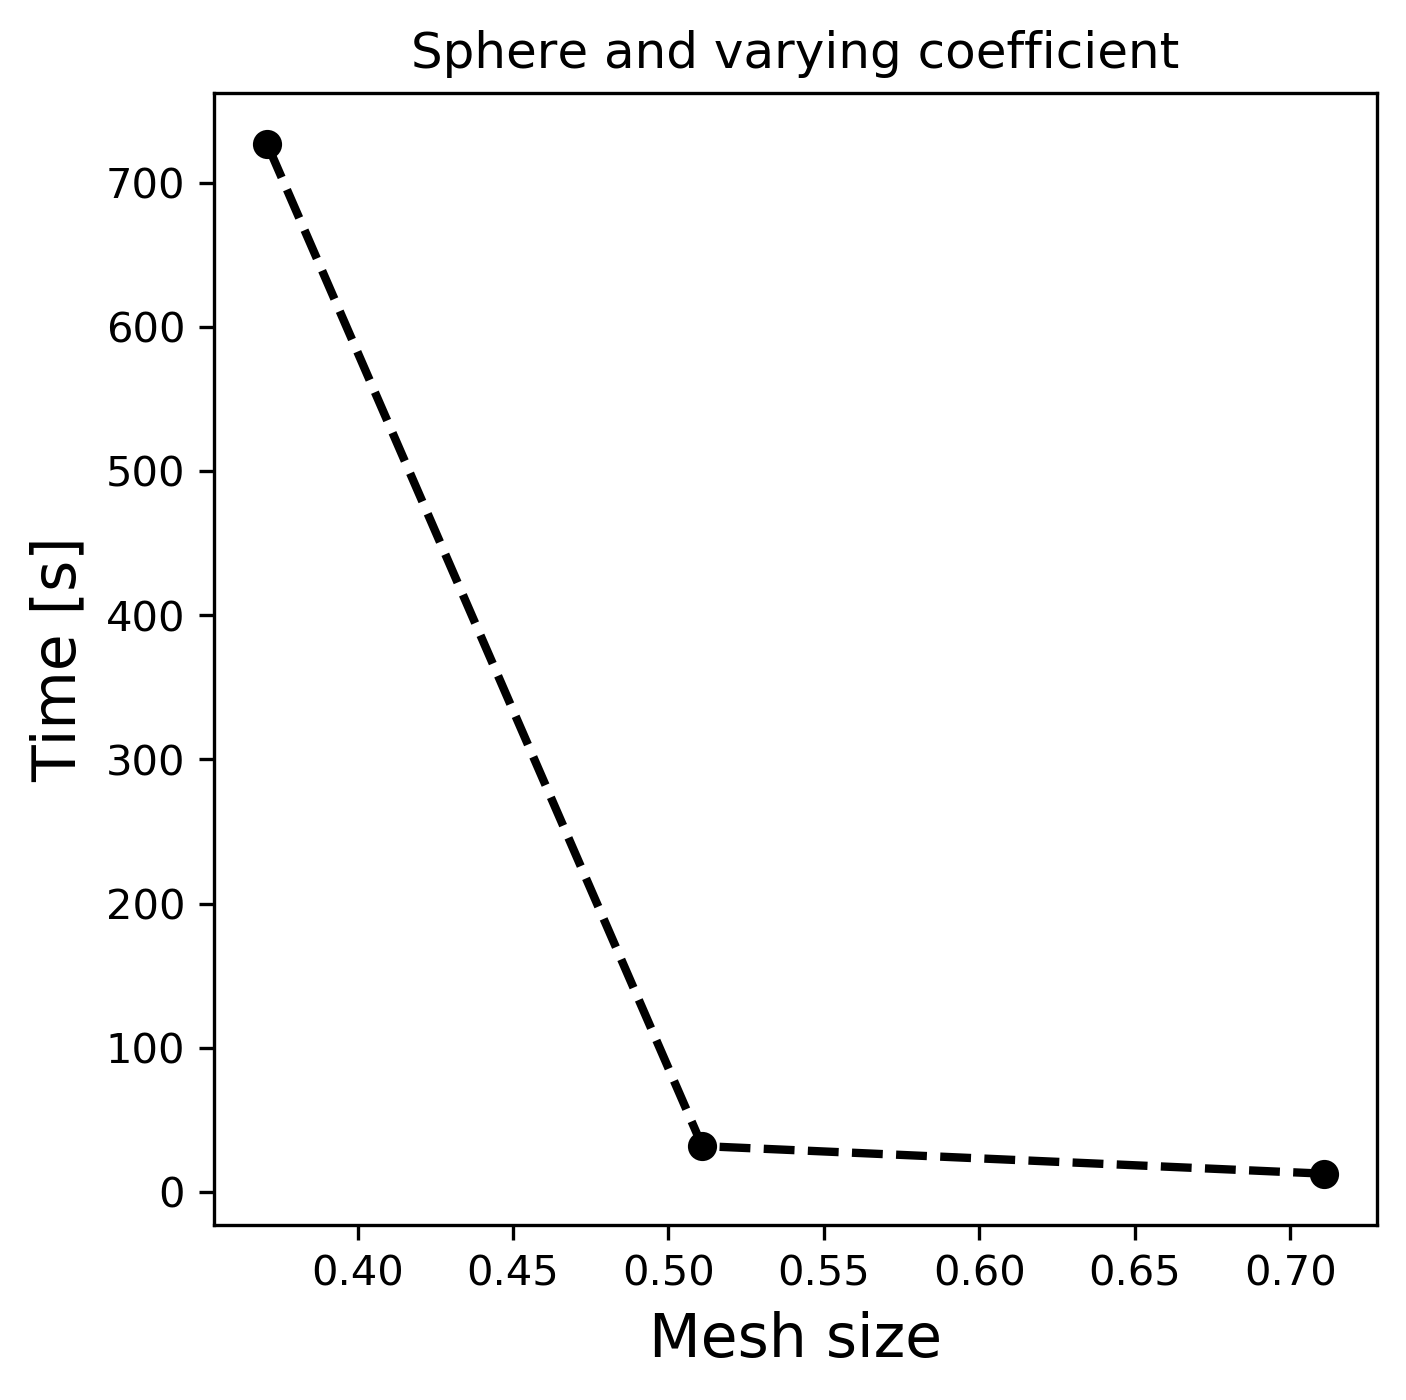
\includegraphics[width=\linewidth]{Hybrid_FEM_BEM_Sphere_varying_coeff_time.png}
%  \caption{Computational time}
%\endminipage
%\end{figure}

%\begin{figure}[!htb]
%\minipage{0.45\textwidth}
%  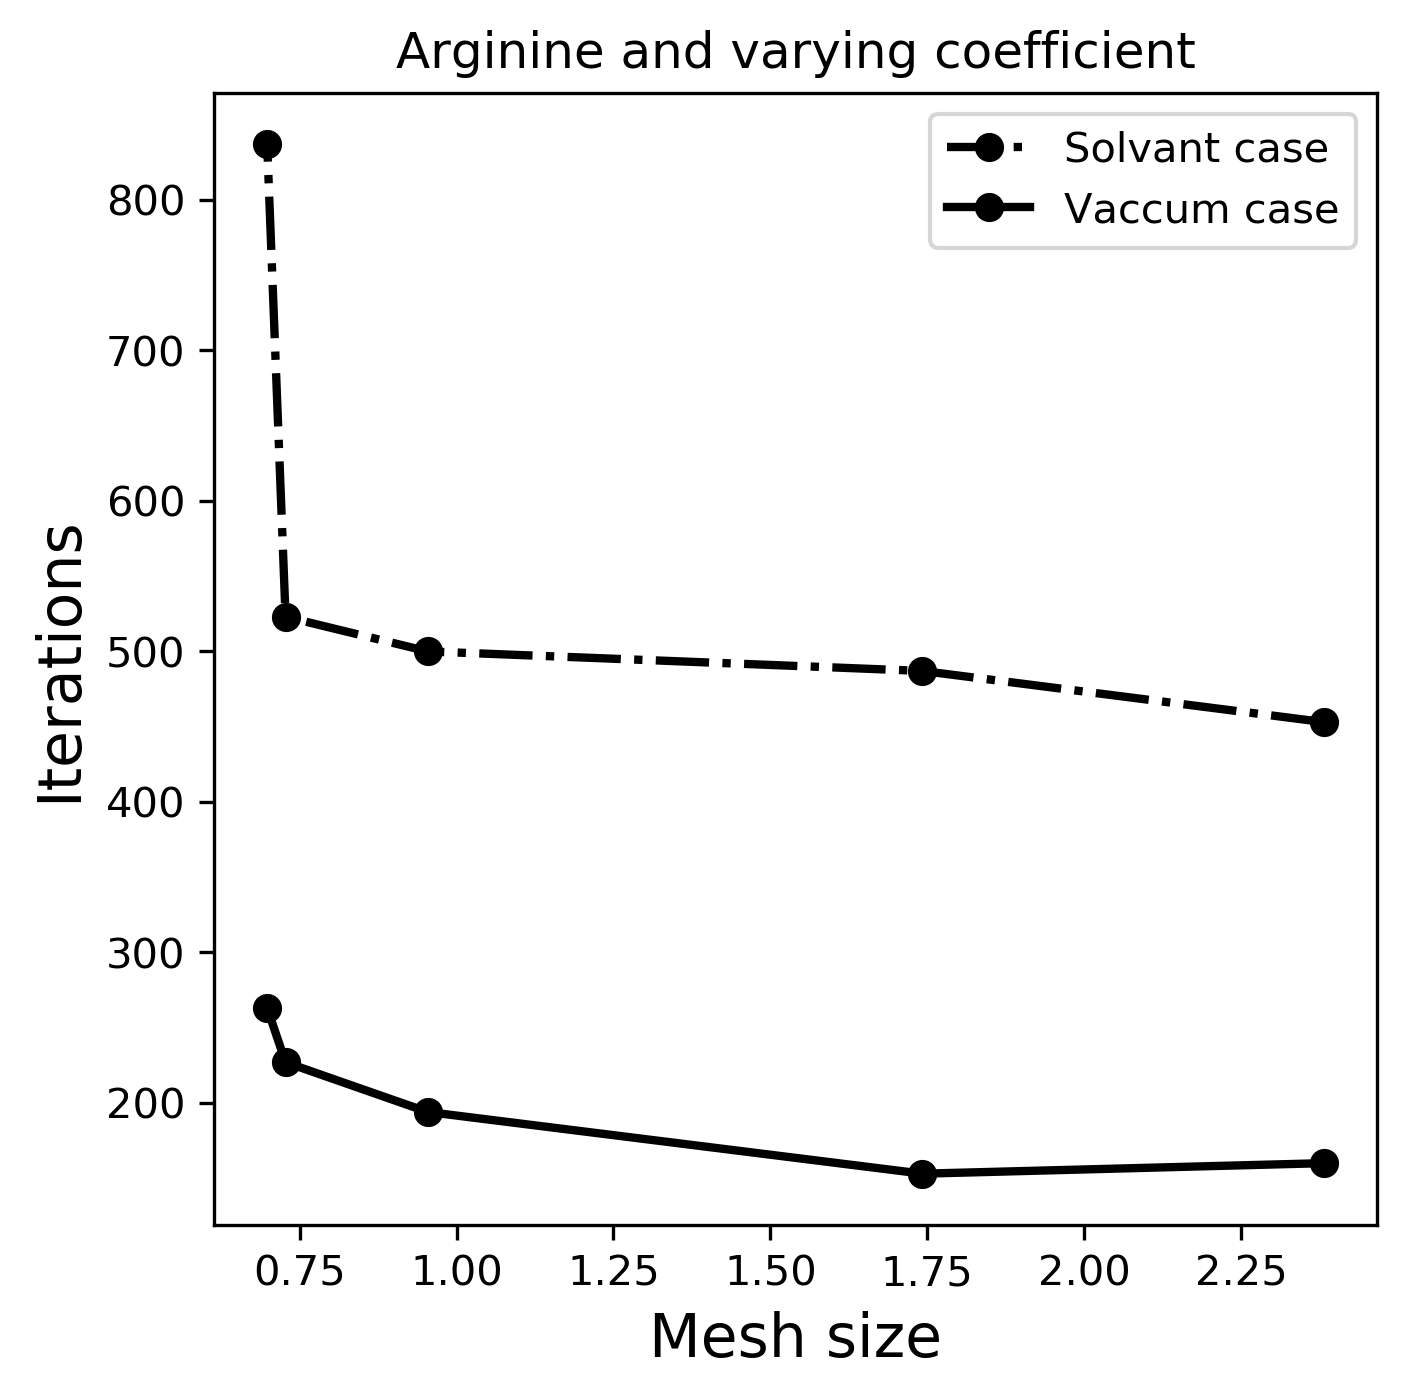
\includegraphics[width=\linewidth]{FEM_BEM_Arginine_varying_coeff_iter.png}
%  \caption{Iterations}
%\endminipage\hfill
%\minipage{0.45\textwidth}%
%  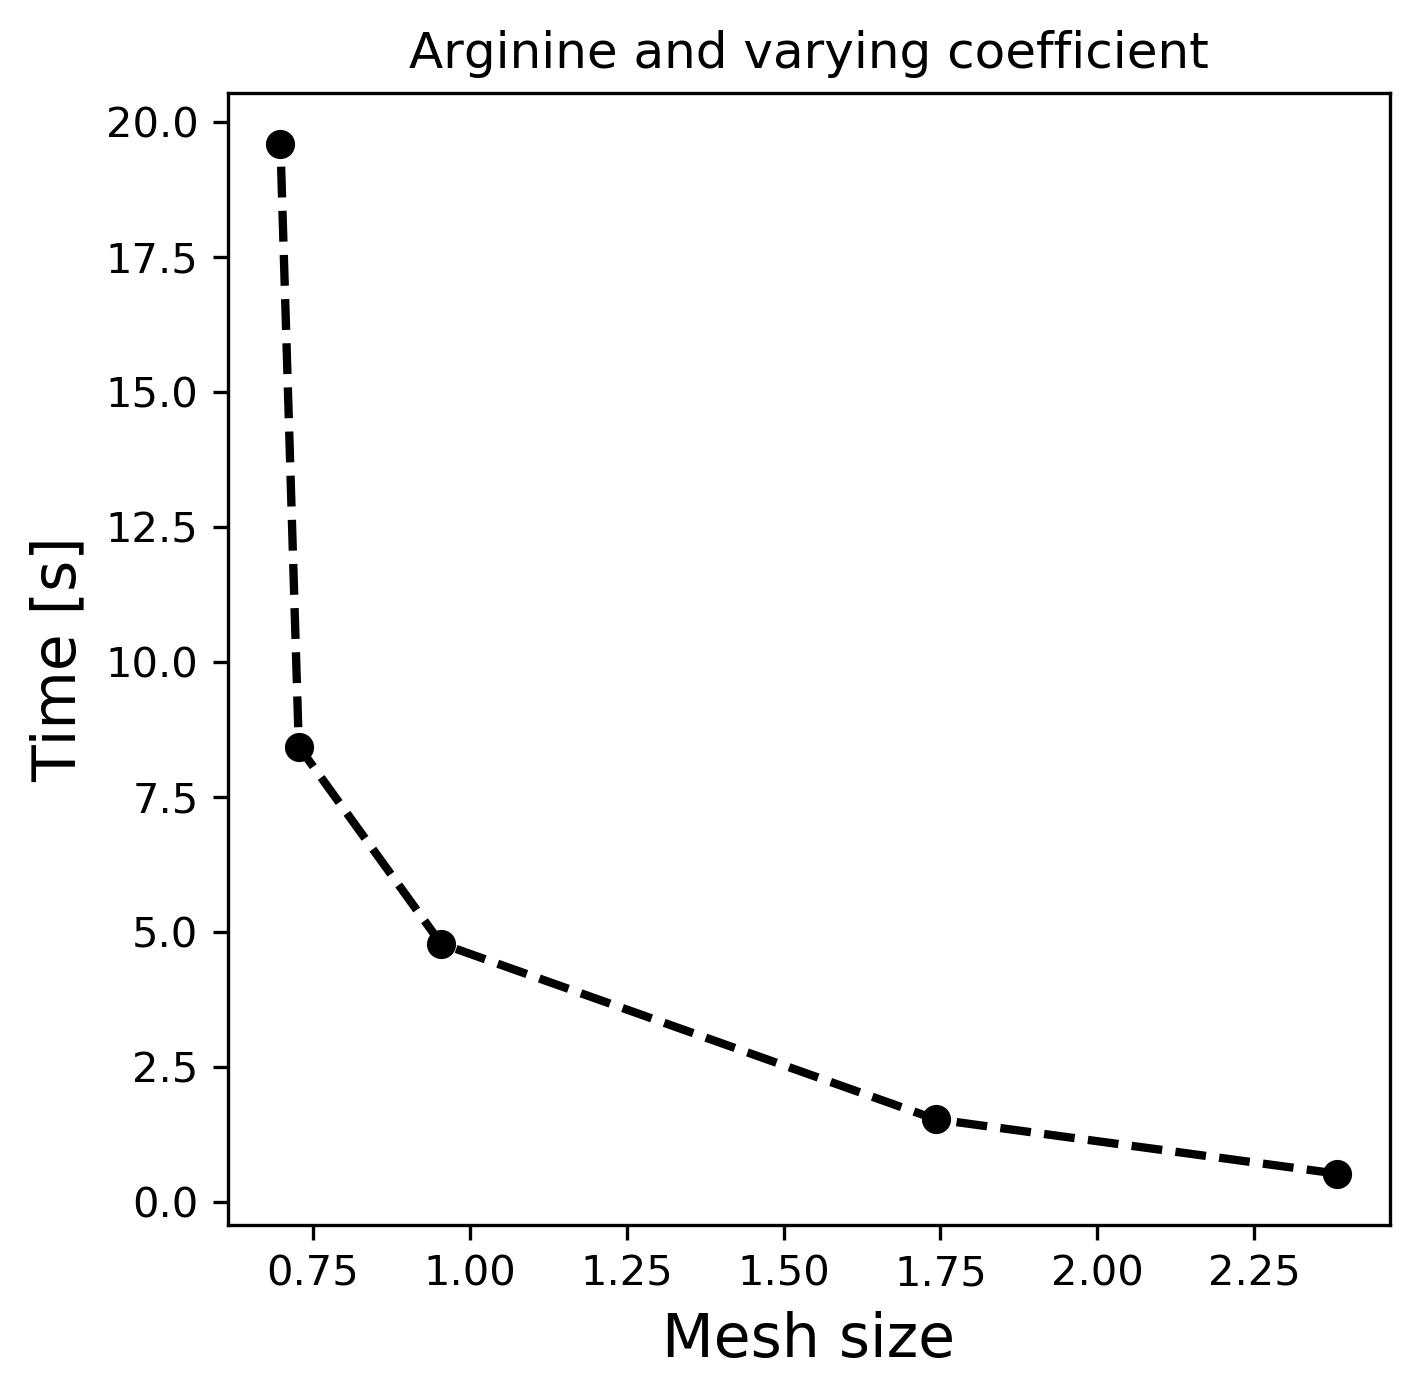
\includegraphics[width=\linewidth]{FEM_BEM_Arginine_varying_coeff_time.png}
%  \caption{Computational time}
%\endminipage
%\end{figure}
%\begin{figure}[!htb]
%\minipage{0.45\textwidth}
%  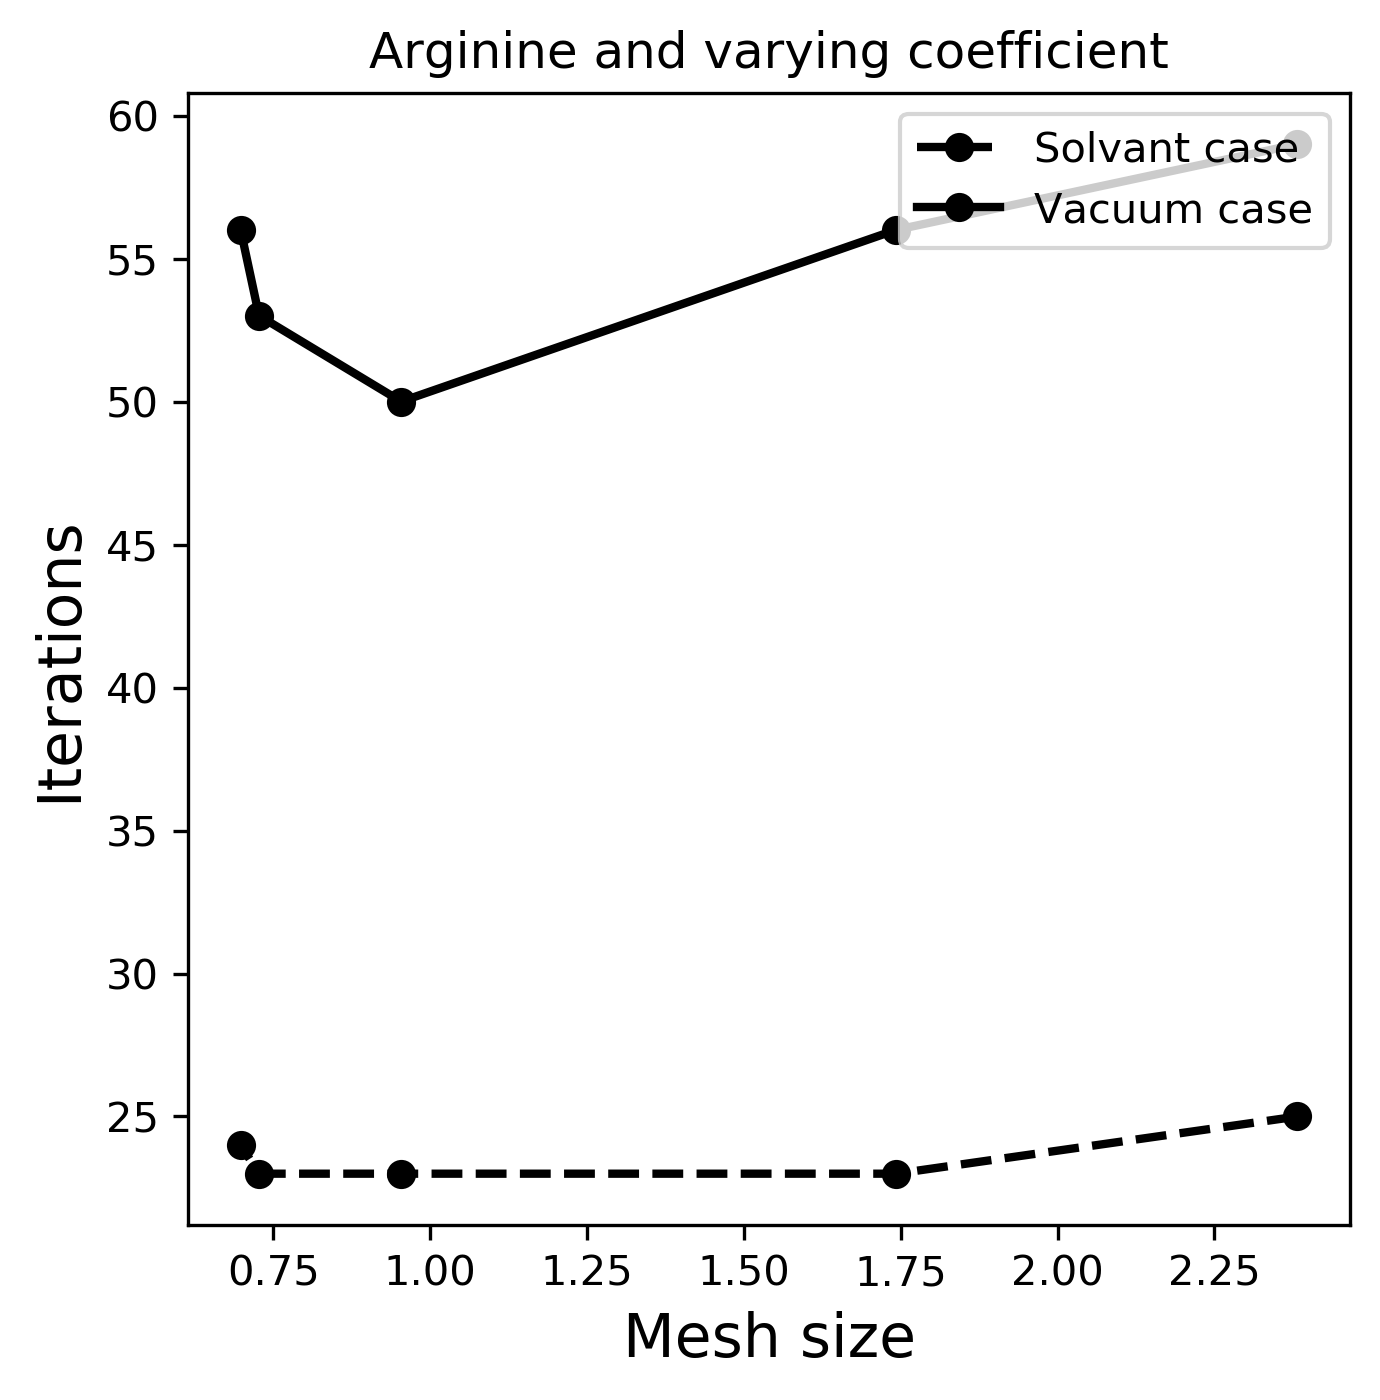
\includegraphics[width=\linewidth]{Hybrid_FEM_BEM_Arginine_varying_coeff_iter.png}
%  \caption{Iterations}
%\endminipage\hfill
%\minipage{0.45\textwidth}%
%  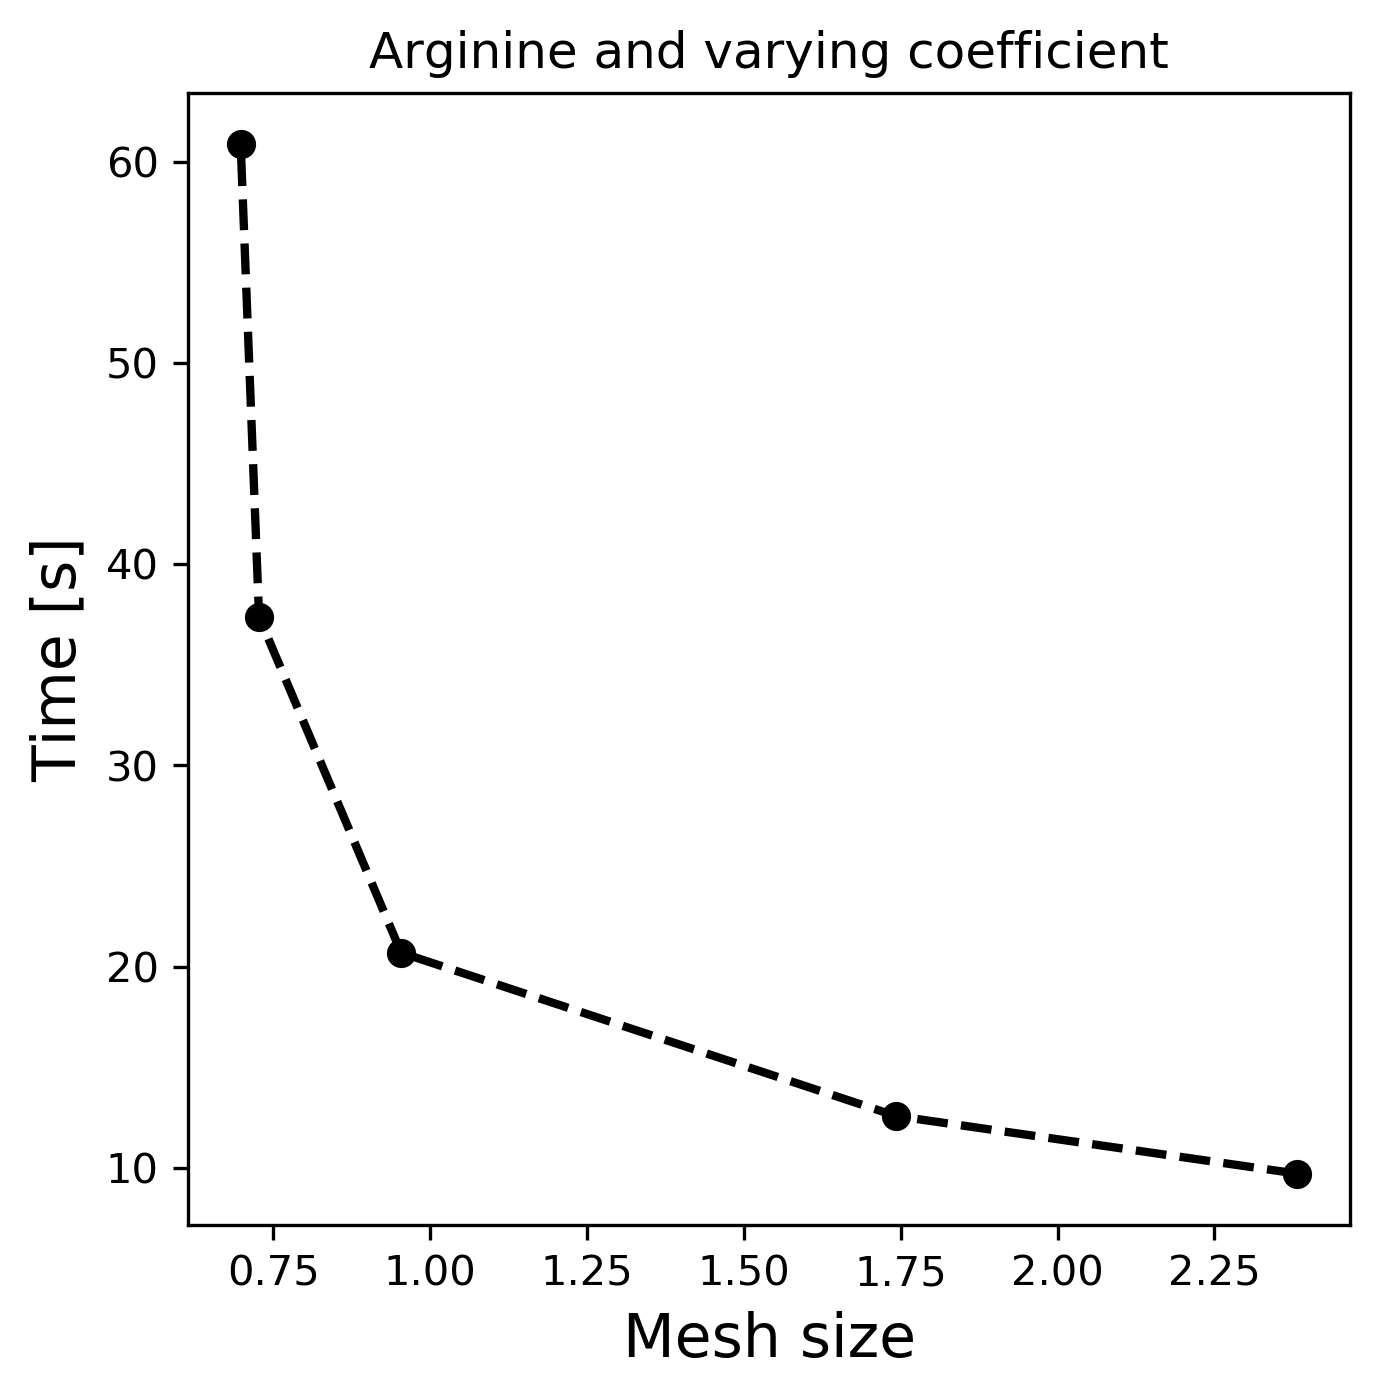
\includegraphics[width=\linewidth]{Hybrid_FEM_BEM_Arginine_varying_coeff_time.png}
%  \caption{Computational time}
%\endminipage
%\end{figure}

\subsection*{\sffamily \large Performance analysis for larger structures}

So far, in all the small structures that we have tested, the standard approach has been more efficient than the hybrid one.
However, the fact that there are better preconditioning strategies for the hybrid approach indicates that it may become faster for larger test cases, where conditioning of the linear system is usually more important. 
In this section, we compare both approaches for larger structures.
